\documentclass{article}
\usepackage[margin=1.2in]{geometry}
\usepackage[T1]{fontenc}
\usepackage[cache=false]{minted}
\usepackage{lmodern, microtype, setspace, hyperref, enumitem, amsmath, amsfonts, xspace, needspace}
\usepackage[nonode]{xgames}
\usepackage[small, bf]{caption}

% Minted
\setminted[latex]{frame=single, linenos, numbersep=4pt, style=tango, breaklines=true, fontsize=\small, tabsize=2}
\setmintedinline[latex]{fontsize=\normalsize}
\renewcommand{\theFancyVerbLine}{\sffamily\textcolor[rgb]{0.7,0.7,0.7}{\scriptsize\arabic{FancyVerbLine}}}

% Boxing examples
\def\posskip{\vskip2pt plus 2pt minus 2pt}
\def\negskip{\vskip-8pt plus 2pt minus 2pt}
\newcounter{fox}
\makeatletter
\def\fox{\@ifstar\@fox\@@fox}
\long\def\@fox#1{\noindent\framebox{\begin{minipage}{0.984\textwidth}#1\end{minipage}}\ignorespaces}
\def\@@fox{\@ifnextchar[{\fox@opt}{\fox@bgt}}
\long\def\fox@bgt#1{\refstepcounter{fox}\noindent\framebox{\begin{minipage}{0.984\textwidth}\hfill{\color{gray}Fig.~\thefox}\par\vspace*{-1.5\baselineskip}#1\end{minipage}}\ignorespaces}
\long\def\fox@opt[#1]#2{\ifstreq@bgt{#1}{a}{\refstepcounter{fox}}{}\noindent\framebox{\begin{minipage}{0.984\textwidth}\hfill{\color{gray}Fig.~\thefox.#1}\par\vspace*{-1.5\baselineskip}#2\end{minipage}}\ignorespaces}
\makeatother
% List
\newenvironment{desc}{\itemize[leftmargin=50pt]}{\enditemize}
\def\macro#1{\item[\cmd{#1}]}
\def\noption#1{\item[\texttt{#1}]}
\def\macroarg#1#2{\item[\cmd{#1}] \hskip-2.5pt\texttt{#2}}
\def\option#1#2{\item[\texttt{#1}] \hskip-1.5pt\texttt{#2}}
\renewcommand{\textbackslash}{\char`\\}
\definecolor{cmd}{HTML}{214a87}
\def\cmd#1{\texttt{\color{cmd}\textbackslash#1}}
\def\leftbrace{\char`\{}
\def\rightbrace{\char`\}}
\def\arg#1{{\color{cmd}\leftbrace}{\color{black}#1}{\color{cmd}\rightbrace}}
\def\optarg[#1]{{\color{player1}[#1]}}
\def\largeskip{\vskip9pt plus 3pt minus 3pt}
\def\TikZ{Ti\emph{k}Z\xspace}

\def\question{\bigskip\noindent\itshape}
\def\answer{\bigskip\noindent\normalshape}

%\def\today{January 12, 2023}

% Document info
\title{\vspace{-7mm}The \textsf{xgames} package\footnote{This file has version number v0.923, last revised on \today.}}
\author{Benjamin Bernard}

\linepenalty1000
\linespread{1.1}
\flushbottom
\setplayercolors{HTML}{c4a100; 3465a4; 4f9905; cf5c00}
\beliefsetoptions{font=\normalsize}


\begin{document}
\maketitle\vspace*{-5mm}

\begin{abstract}
This is a game theory package that places emphasis on user-friendly input and coloring each player's name, actions, and payoffs in a dedicated color for ease of distinction.
\end{abstract}

\section{Introduction}

There are a few options out there to create \LaTeX\ renditions of game trees or normal-form games:
\begin{itemize}
\item Packages \texttt{sgamex} and \texttt{egameps} by Martin J.~Obsorne.
\item Package \texttt{istgame} by In-Sung Cho. 
\item The \texttt{trees} or \texttt{positioning} libraries of \TikZ.
\end{itemize}
What sets this package apart from the above is that it provides an integrated package for writing full examples, lecture slides, or assignments questions, in which each player's name, actions, and payoffs are typeset in a dedicated color for ease of distinction. All commands are overlay aware so that game trees, normal-form games, belief spaces, and automata can be revealed gradually in class. Moreover, I placed great emphasis on making the input user-friendly. Finally, there are some gimmicky options like drawing the players' payoffs after a payoff matrix has been parsed or displaying the distribution that a strategy profile induces on a game tree. 
%
For a comparison of the different packages' ease of use, see Section~\ref{sec:Comparison}.

\section{Instructions for the Impatient}

\subsection{Installation}

While you could just copy and paste the style files \texttt{xgames.sty} and \texttt{fikz.sty} into your current working directory, it is neater to install those style files in a local TeXMF root directory so that they are accessible in any working directory. To set up a some folder \texttt{mytexmf} as a root directory in MiKTeX, add it to the list of directories in the settings of the MiKTeX console and copy each \texttt{package.sty} into the subfolder \texttt{mytexmf/tex/latex/package/}. Specifically, for this package place \texttt{xgames.sty} and \texttt{fikz.sty} into subfolders \texttt{mytexmf/tex/latex/xgames/} and \texttt{mytexmf/tex/latex/fikz/}, respectively. 

\subsection{Reading this Documentation Quickly}

This package is built on \TikZ and its macros work in any regular \texttt{tikzpicture} environment. For best use, the package provides dedicated environments \texttt{matrixgame}, \texttt{beliefspace}, \texttt{gametree}, and \texttt{automaton} that locally redefine some styles and make it easier to customize figures by specifying key-value pairs for the entire figure. All macros form this package and from \TikZ work in any of the dedicated environments, thereby allowing one to create hybrid figures easily.

For a brief introduction on how to implement normal-form games, belief spaces, extensive-form games, and automata, have a look at the examples in Section~\ref{sec:Examples}. The examples explain a majority of the package's functionality at a quick glance. The commands and keys are explained following the example in which they appear the first time. In order to tweak those examples to your liking, you can check the full discussion of the commands and their options in Section~\ref{sec:Usage}. There is quite a bit of repetition between Sections~\ref{sec:Examples} and~\ref{sec:Usage}. The main goal was to reduce search time rather than to produce a short document.

To get started as quickly as possible, load the package with the \texttt{nonode} option to improve the compilation speed of game trees by about 10\%. With this option, nodes of a game tree are implemented as a circle-shaped path instead of a full-fledged \TikZ node. As a consequence, \TikZ paths ending in such a node will not be shortened, but rather end behind the node's center. The output of all commands from this package will look identical with or without the \texttt{nonode} option, but if you intend to mark up the trees with arrows, for example, you may wish to load the package without this option. This documentation, in fact, has been typeset with the \texttt{nonode} option.

Error handling is still utterly absent from this package. I apologize for any frustration caused.

\section{Examples}\label{sec:Examples}

\subsection{Normal-Form Games and Text Markup}

\fox{
\begin{center}\posskip
\begin{matrixgame}[top={L, R}, left={U, D}, bottom={A, B}]
	\payoffmatrix{0, 3, 1 & 0, 2, 2\\ 2, \br<3->{1}, \br<4->{4} & 2, 0, 1}
	\payoffmatrix[pos={5,0}]{2, 2, 3 & 0, 1, 2\\ 3, 0, 1 & 1, \br<3->{2}, \br<4->{2}}
	\strike<2->{h}{1}
\end{matrixgame}
\end{center}\negskip

For \pl1, strategy $\pl1{U}$ is strictly dominated by strategy $\pl1{D}$. No other pure strategies are iteratively dominated. The pure strategies that survive IESDS are $\plset1{D}$ for \pl1, $\plset2{L, R}$ for \pl2, and $\plset3{A, D}$ for \pl3. There are two pure-strategy Nash equilibria $\ap{D, L, A}$ and $\ap{D, R, B}$.\label{matrix:basic}
}

\begin{minted}{latex}
\begin{center}
\begin{matrixgame}[top={L, R}, left={U, D}, bottom={A, B}]
	\payoffmatrix{0, 3, 1 & 0, 2, 2\\ 2, \br<3->{1}, \br<4->{4} & 2, 0, 1}
	\payoffmatrix[pos={5,0}]{2, 2, 3 & 0, 1, 2\\ 3, 0, 1 & 1, \br<3->{2}, \br<4->{2}}
	\strike<2->{h}{1}
\end{matrixgame}
\end{center}

For \pl1, strategy $\pl1{U}$ is strictly dominated by strategy $\pl1{D}$. No other pure strategies are iteratively dominated. The pure strategies that survive IESDS are $\plset1{D}$ for \pl1, $\plset2{L, R}$ for \pl2, and $\plset3{A, D}$ for \pl3. There are two pure-strategy Nash equilibria $\ap{D, L, A}$ and $\ap{D, R, B}$.
\end{minted}
\vspace{-1.5mm}

%\newpage
The main macro to typeset normal-form games is \cmd{payoffmatrix}, to which the input is provided as in a regular \texttt{tabular} environment. The key \texttt{pos=\arg{5,0}} offsets the center of the second payoff matrix by $(5, 0)$ in the \TikZ coordinate system that underlies the \texttt{matrixgame} environment. Labels provided as a comma-separated list to the keys \texttt{top}, \texttt{left}, and \texttt{bottom} are added to all payoff matrices of this \texttt{matrixgame}. The \cmd{strike} command strikes out a player's strategy in all payoff matrices. Here, \texttt{h} in the first argument stands for horizontal. With arguments \texttt{v} and \texttt{x}, strategies of players~$2$ and~$3$ can be struck through. Best responses are highlighted using \cmd{br}. Both \cmd{strike} and \cmd{br} are overlay aware. 

The commands \cmd{pli} for $i = 1, \ldots, 9$ color any text in player~$i$'s color.\footnote{Formally, the macro is a single-argument macro \cmd{pl\arg{<num>}} that scans for a second argument with a \cmd{futurelet} command. We can omit the braces around \texttt{<num>} because it is a single token.}\setmintedinline[latex]{fontsize=\normalsize}
%
The color palette can be changed by \cmd{setplayercolors} or \cmd{letplayercolors}. For example, the preamble of this file contains the line \cmd{setplayercolors\arg{HTML}\arg{c4a100; 3465a4; 4f9905; cf5c00}} to match the ``tango'' color scheme of the \texttt{minted} package. Without argument, the command \cmd{pli} prints player~$i$'s name, which is ``Player~$i$'' by default. The commands \cmd{plseti} for $i = 1, \ldots, 9$ color the elements of a comma-separated list in player~$i$'s color. Action profiles or payoff vectors can be colored by passing the player's actions or payoffs, respectively, as a comma-separated list to \cmd{ap} (short for action profile).\largeskip

%\subsection{Repeated games}

\fox{
\begin{center}\posskip
\begin{matrixgame}[force math, top={h,\ell}, left={H,L}, player names={Firm,Customer}, br]
	\payoffmatrix[w=1.3, h=0.75]{2, 3 & 0, 2\\ 3, 0 & 1, 1}
	\drawpayoffs[scale=0.75, shift={5,-0.8}]
\end{matrixgame}
\end{center}\negskip

\definevar{H, L; h, \ell}
A long-lived \pl1 chooses to exert a ($\H$)igh or a ($\L$)ow amount of effort and the short-lived \pl2 chooses to buy a ($\h$)igh-priced or a ($\ell$)ow-priced product.\label{matrix:advanced}
\releasevar
}


\begin{minted}{latex}
\begin{center}
\begin{matrixgame}[force math, top={h,\ell}, left={H,L}, player names={Firm,Customer}, br]
	\payoffmatrix[w=1.3, h=0.75]{2, 3 & 0, 2\\ 3, 0 & 1, 1}
	\drawpayoffs<2->[scale=0.75, shift={5,-0.8}]
\end{matrixgame}
\end{center}

\definevar{H, L; h, \ell}
A long-lived \pl1 chooses to exert a ($\H$)igh or a ($\L$)ow amount of effort and the short-lived \pl2 chooses to buy a ($\h$)igh-priced or a ($\ell$)ow-priced product.
\releasevar
\end{minted}
\vspace{-1mm}


The key \texttt{force math} places action labels in all payoff matrices and drawn payoffs in math mode. The key \texttt{player names=\arg{Firm, Customer}} changes the players' names globally and adds the players' names to the payoff matrix. When the key \texttt{br} is passed to \cmd{payoffmatrix}, all best responses are highlighted automatically with \cmd{br}, given that payoffs are explicit numbers and there are three or fewer players. The keys \texttt{w} and \texttt{h} govern the width and height of the cells, respectively. The command \cmd{drawpayoffs} draws the pure-action stage game payoffs of a two-player game parsed with \cmd{payoffmatrix} as well as their convex hull. The key \texttt{scale=<factor>} scales the drawn image by \texttt{<factor>} and the key \texttt{shift=\arg{x,y}} shifts the origin by $(x, y)$ from the center of the payoff matrix.

Instead of writing \cmd{pli\arg{<text>}} to refer to player~$i$'s action \texttt{<text>}, one can also define commands \cmd{<text>} using \cmd{definevar}. Players are separated by semicolons and each player's actions by commas. If any existing macros are overridden by \cmd{definevar}, they are restored by \cmd{releasevar}. Below four examples show four more ways, with which one can quickly colorize text by players.\largeskip


\fox*{
\setplayernames{Principal, Agent}
\definevar[player=2]{\alpha, \A->\mathcal{A}}
If the \pl2's action $\alpha \in \A$ is observed by the \pl1, the \pl1 can incentivize the \pl2 to choose his/her preferred action $\alpha_{\ast}$ by making the payment conditional on the observed action.
\releasevar{\alpha, \A}
}

\begin{minted}{latex}
\setplayernames{Principal, Agent}
\definevar[player=2]{\alpha, \A->\mathcal{A}}
If the \pl2's action $\alpha \in \A$ is observed by the \pl1, the \pl1 can incentivize the \pl2 to choose his/her preferred action $\alpha_{\ast}$ by making the payment conditional on the observed action.
\releasevar{\alpha, \A}
\end{minted}
\vspace{-1mm}

If the variable to be defined is a command sequence, the content of that command sequence is typeset in the player's color. One can set the variable to any arbitrary content with the notation \cmd{variable}\texttt{-><content>}. Note that subscripts are absorbed in the color of the variable as it is interpreted as different instance of the same variable. By setting the key \texttt{player=<num>}, the first variable is parsed as player~\texttt{<num>}'s variable and the player counter increases with each semicolon. In this instance, the same effect could be achieved by \cmd{definevar\arg{; \cmd{alpha}, \cmd{A}->\cmd{mathcal}\arg{A}}}. If one wishes to release only some, but not all variables defined by \cmd{definevar}, one can pass a comma-separated list to \cmd{releasevar} of variables to be released. Doing so is marginally slower than releasing all variables at once and certain auxiliary macros will not be released (such as \cmd{qhat} in below example). It is thus recommended to simply release all variables at once at the end of an example.\largeskip

\fox*{
\setplayernames{Firm~1, Firm~2}
\multivar{u}
\multivar[prefix=hat, postfix=']{q}
Since $\u1'(\qhat1, \qhat2) > 0$, \pl1 has an incentive to deviate and produce a quantity $\q1' > \qhat1$.
\releasevar
}

\begin{minted}{latex}
\setplayernames{Firm~1, Firm~2}
\multivar{u}
\multivar[prefix=hat, postfix=']{q}
Since $\u1'(\qhat1, \qhat2) > 0$, \pl1 has an incentive to deviate and produce a quantity $\q1' > \qhat1$.
\releasevar
\end{minted}
\vspace{-1mm}

%The command \cmd{apm} colors a comma-separated list by player colors as displayed in a \cmd{payoffmatrix} (hence the \texttt{m} in \cmd{apm}). 
The command \cmd{multivar} defines macros \cmd{<text>i} for $i = 1, \ldots, 9$ which typeset \verb|<text>_i| in player~$i$'s color. It is possible to refer to different instances of the same variable by setting the \texttt{prefix} and the \texttt{postfix} keys. The key \texttt{prefix=<prefix>} defines macros \cmd{<text><prefix>i}, which are typeset as \cmd{<prefix>\arg{<text>}}\verb|_i|. Instead of \texttt{hat}, one could use it to typeset \texttt{tilde}, \texttt{bar}, \texttt{underline}, \texttt{mathcal}, etc. To denote different instances by superscripts or primes, set the \texttt{postfix} key to \verb|^|, \verb|'|, or \verb|{^,'}|, respectively. Contrary to subscripts, superscripts or primes are not absorbed in the player's color by default because they could signify powers or derivatives. Again, \cmd{releasevar} restores any macros that have been overwritten, including hats, bars, tildes, etc.\largeskip

\fox*{
\setplayernames{Incumbent, Challenger}
\multivar[index=initial]{\beta}
The \pl1 and the \pl2 choose a campaign budget $\beta1$ and $\beta2$, respectively. The probability of winning depends on the entire profile $\beta0 = (\beta1, \beta2)$.
\releasevar
}

\begin{minted}{latex}
\setplayernames{Incumbent, Challenger}
\multivar[index=initial]{\beta}
The \pl1 and the \pl2 choose a campaign budget $\beta1$ and $\beta2$, respectively. The probability of winning depends on the entire profile $\beta0 = (\beta1, \beta2)$.
\releasevar
\end{minted}
\vspace{-1mm}

By passing the key-value pair \texttt{index=initial} to \cmd{mutlivar}, the player's actions are indexed by the first letter of their names instead. By passing player number~0, coloring and subscripts are suppressed. Alternatively, the same effect could be achieved by declaring \cmd{multivar\optarg[index=initial]\arg{\cmd{b}->\cmd{beta}}} before the example and by writing \cmd{beta}\texttt{ = (\cmd{b1}, \cmd{b2})} in the example. %See Section~\ref{sec:Usage} for a reference of all key-value pairs that \cmd{mutlivar} takes.
\largeskip

\fox*{
\resetplayernames
Players~$i = \apm{1, 2}$ choose $a_i \in \textset{Rock, Paper, Scissors}$. \pl1's best response is $\BR[1](\pltext2{Rock}) = \textset1{Paper}$.
\releasevar
}

\begin{minted}{latex}
\resetplayernames
Both players~$i = \apm{1, 2}$ choose $a_i \in \textset{Rock, Paper, Scissors}$. \pl1's best response is $\BR[1](\pltext2{Rock}) = \textset1{Paper}$.
\releasevar
\end{minted}
\vspace{-1.5mm}

The players' names can be reset to default with \cmd{resetplayernames}. %This differs from \cmd{setplayernames\arg{Player~1, Player~2}} in that it resets the player~$i$'s ``initial'' to $i$, whereas the latter would set it to $P$ for every player. 
The command \cmd{apm} colors a comma-separated list by player colors as displayed in a \cmd{payoffmatrix} (hence the \texttt{m} in \cmd{apm}). Actions and sets of actions that are spelled out, rather than abbreviated by variables, can be typeset with the commands \cmd{pltexti}, \cmd{textset}, and \cmd{textseti} for $i = 1, \ldots, 9$. The command $\cmd{BR\optarg[i]}$ is intended for typesetting player~$i$'s best response correspondence.\largeskip

\fox{
\begin{center}\posskip
\definevar{x; ; z}
\begin{matrixgame}[top={L, R}, left={U, D}, bottom={A, B}]
	\payoffmatrix{0, 3, 1 & 0, 2, 2\\ 2, 1, 4 & 2, 0, 1}
	\payoffmatrix[pos={5,0}]{2, 2, 3 & 0, 1, 2\\ 3, 0, 1 & 1, 2, 2}
	\probmatrix<2->{\x, *; 1, 0; \z, *}
\end{matrixgame}
\releasevar
\end{center}\vspace{-3mm}
}

\begin{minted}{latex}
\definevar{x; ; z}
\begin{matrixgame}[top={L, R}, left={U, D}, bottom={A, B}]
	\payoffmatrix{0, 3, 1 & 0, 2, 2\\ 2, 1, 4 & 2, 0, 1}
	\payoffmatrix[pos={5,0}]{2, 2, 3 & 0, 1, 2\\ 3, 0, 1 & 1, 2, 2}
	\probmatrix<2->{\x, *; 1, 0; \z, *}
\end{matrixgame}
\releasevar
\end{minted}
\vspace{-1.5mm}

The distribution over outcomes induced by a mixed strategy profile can be shown with the \cmd{probmatrix} command. Players are separated by a semicolon, probabilities of individual pure strategies by the same player are separated by a comma. Use an \texttt{$\ast$} to fill in the complementary probability.\largeskip %Same as the other commands used to typeset normal-form games, \cmd{probmatrix} is overlay aware and it is limited to three players. See Section~\ref{sec:Matrixgame} for customization options.\largeskip

\fox{
\begin{center}
\matrixsetoptions{w=1.2}
\begin{matrixgame}[top left={A, B}]
	\payoffmatrix{0 & 1 \\ 2 & -1}
\end{matrixgame}
\hspace{5mm}
\matrixsetoptions{single player=nature}
\begin{matrixgame}[top={H, L}, left={A, B}]
	\payoffmatrix{0 & 1 \\ 2 & -1}
\end{matrixgame}
\hspace{5mm}
\begin{matrixgame}[top left={A, B}, zero-sum]
	\payoffmatrix{0 & 1 \\ 2 & -1}
\end{matrixgame}\label{matrix:zero-sum}
\end{center}\vspace{-1.5mm}
}

\begin{minted}{latex}
\matrixsetoptions{w=1.2}
\begin{matrixgame}[top left={A, B}]
	\payoffmatrix{0 & 1 \\ 2 & -1}
\end{matrixgame}
\matrixsetoptions{single player=nature}
\begin{matrixgame}[top={H, L}, left={A, B}]
	\payoffmatrix{0 & 1 \\ 2 & -1}
\end{matrixgame}
\begin{matrixgame}[top left={A, B}, zero-sum]
	\payoffmatrix{0 & 1 \\ 2 & -1}
\end{matrixgame}
\end{minted}
\vspace{-1mm}

The key \texttt{single player} determines how the game is colored when payoffs of only a single player are displayed. Shown above are three matrices for the values \texttt{default}, \texttt{nature}, and \texttt{zero-sum}, respectively. Those values can be set locally, for a single \texttt{matrixgame} environment or globally through the command \cmd{matrixsetoptions}. Alternatively, the colors of the cell entries and labels can be customized with the \texttt{color} or \texttt{player} keys; see Section~\ref{sec:Matrixgame} for further examples.\largeskip


\fox{\posskip
\setplayernames{Entrant, Incumbent}
\begin{center}
\begin{matrixgame}[name=startup, players, w=1.4, strike width=1.5pt, immediate]
	\payoffmatrix[w={1.6, 1.2}]{-1, 1.5 & 1, 2 \\ 0, 3.5 & 0, 3}
	\payoffmatrix[pos={5.5, 0}]{-1, 0 & 1, 2 \\ 0, 2 & 0, 3}
	\toplabel{I, N}
	\leftlabel{E, N}
	\bottomlabel[list sep=;]{$u(\vartheta_L, a)$; $u(\vartheta_H, a)$}
	\strike[2]{v}{1}
	\draw[player1, thick, rounded corners=8.5] (3.52, -0.7) rectangle (7.1, -0.1);
	\begin{pgfinterruptboundingbox}
		\node[player1, right, font=\footnotesize] at (7.1, -0.4) {not dominated};
	\end{pgfinterruptboundingbox}
\end{matrixgame}\label{matrix:immediate}
\end{center}
}

\Needspace*{4\baselineskip}

\begin{minted}{latex}
\setplayernames{Entrant, Incumbent}
\begin{matrixgame}[name=startup, players, w=1.4, strike width=1.5pt, immediate]
	\payoffmatrix[w={1.6, 1.2}]{-1, 1.5 & 1, 2 \\ 0, 3.5 & 0, 3}
	\payoffmatrix[pos={5.5, 0}]{-1, 0 & 1, 2 \\ 0, 2 & 0, 3}
	\toplabel{I, N}
	\leftlabel{E, N}
	\bottomlabel[list sep=;]{$u(\vartheta_L, a)$; $u(\vartheta_H, a)$}
	\strike<2->[2]{v}{1}
	\draw<3->[player1, thick, rounded corners=8.5] (3.52, -0.7) rectangle (7.1, -0.1);
	\node<3->[player1, right, font=\footnotesize] at (7.1, -0.4) {not dominated};
\end{matrixgame}
\end{minted}
\vspace{-1mm}

If the labels are passed to the \texttt{matrixgame} as key-value pairs, they are typeset at the end of the environment to ensure that all payoff matrices have been parsed. Since the \cmd{strike} and the \cmd{drawpayoffs} commands require access to those labels, their output is drawn only at the end of the environment by default, regardless of when their input is parsed. In order to mark up the image above any \cmd{strike}s, we use the \texttt{immediate} key. This key causes the commands \cmd{strike} and \cmd{drawpayoffs} to be typeset as they are parsed. Passing this key necessitates that:
\begin{itemize}
\item Top, left, and bottom labels are issued with their separate commands \textit{after} all payoff matrices have been parsed and \textit{before} any \cmd{strike} or \cmd{drawpayoffs} commands are issued.
\item If the key \texttt{br} is set, it is set for an individual \cmd{payoffmatrix} of at most two players (because best responses by player~3 cannot be determined matrix by matrix).
\end{itemize} 
The key \texttt{immediate} is always active in regular \texttt{tikzpicture} environments. Any environments of this package can be marked up by any \TikZ commands such as the \cmd{draw} and \cmd{node} commands on lines 9--10. In such commands, player~$i$'s color can be accessed by the color \texttt{playeri}.

The \cmd{strike} width and many other options can be customized by passing them as environment options. See Section~\ref{sec:Usage} for a comprehensive list. \cmd{strike} takes an optional argument \texttt{<number>} if a strike is to be drawn in only one matrix. If the players' names have been defined before the \texttt{matrixgame} environment, such as through \cmd{setplayernames\arg{<list of names>}} before the \texttt{center} environment here, you can display those names with the  \texttt{players} key instead of setting them again with the \texttt{player names} key as in Figure~\ref{matrix:advanced}. Column widths can be adjusted individually with the key \texttt{w=\arg{<list of widths>}}. The key \texttt{h=\arg{<list of heights>}} individually adjusts the height of rows.

The command \cmd{bottomlabel} behaves differently for 2-player and 3-player games. In 2-player games, \cmd{bottomlabel} is interpreted as a description of states rather than the actions of a third player. It is thus unaffected by the \texttt{force math} key, it is typeset in the package foreground color \texttt{xg-fg} by default, and it is separated slightly further from the \cmd{payoffmatrix} than player~3's action labels would be. In order to attain the same label distance as from payoff matrices in 3-player games, pass the key \texttt{tight}. The list separator of any label command can be changed with the \texttt{list sep} key. This is convenient if any of the labels contain a comma, the default separator of lists. If the \texttt{list sep} key is passed at the environment level, it is changed for all labels, including labels set through key-value pairs.

%\newpage
\subsection{Payoff Sets}

%\statesetoptions{base line=false}
\fox{\posskip
\begin{center}
\begin{tikzpicture}
	\drawpayoffs[name=startup, matrix=2, force math, axis=1.25]
\end{tikzpicture}
\hspace{2cm}
\begin{tikzpicture}
	\draw[edge, -latex] (-1.3, 0) -- (1.4, 0);
	\draw[edge, -latex] (0, 0) -- (0, 3.7);
	\state (EN) at (1, 2) <2->{$\ap{E, N}$};
	\state[label=260] (EI) at (-1, 0) {$\ap{E, I}$};
	\state[label=175] (NN) at (0, 3) {$\ap{N, N}$};
	\state[left, contour=delay] (NI) at (0, 2) {$\ap{N, I}$};
	\draw[edge] (EN) -- (NN) -- (EI) -- (EN);
\end{tikzpicture}\label{drawpayoffs}
\end{center}
}

\begin{minted}{latex}
\begin{tikzpicture}
	\drawpayoffs[name=startup, matrix=2, force math, axis=1.25]
\end{tikzpicture}
\begin{tikzpicture}
	\draw[edge, -latex] (-1.3, 0) -- (1.4, 0);
	\draw[edge, -latex] (0, 0) -- (0, 3.7);
	\state (EN) at (1, 2) <2->{$\ap{E, N}$};
	\state[label=260] (EI) at (-1, 0) {$\ap{E, I}$};
	\state[label=175] (NN) at (0, 3) {$\ap{N, N}$};
	\state[left, contour=delay] (NI) at (0, 2) {$\ap{N, I}$};
	\draw[edge] (EN) -- (NN) -- (EI) -- (EN);
\end{tikzpicture}
\end{minted}
\vspace{-1mm}

To align payoff sets vertically centered with the matrixgame that defines the payoffs, it is easiest to draw payoffs in a separate \texttt{tikzpicture} environment rather than in the same \texttt{matrixgame}. You can store any parsed \texttt{matrixgame} with the option \texttt{name=<text>} and recall it with \texttt{name=<text>} in \cmd{drawpayoffs}. The key \texttt{matrix=<number>} determines which \cmd{payoffmatrix} of the environment is drawn. Without the \texttt{name} key, the most recent unnamed \texttt{matrixgame} is drawn.\footnote{In this instance, the payoff pairs of the first two players in the second matrix parsed in Figure~\ref{matrix:basic} would be drawn. Labels, however, would be taken from the product-choice game because they are overwritten.} If payoffs are drawn in a separate environment, the key \texttt{force math} needs to be re-issued. The key \texttt{axis=<factor>} determines how far beyond the maximum payoffs the axes extend. Labels of each payoff pair are drawn on the opposite side of the center of mass among payoff pairs. This will look good in many repeated games we teach, but in some games (as above) it may not. Labels can be turned off with the key \texttt{labels=off}.

It is not difficult (and instructive) to draw this payoff set manually. The syntax of the \cmd{state} command is identical to a \TikZ \cmd{node} with two exceptions: braces are optional if no label is to be set and a separate overlay instruction \texttt{<overlay>} can be given to the label. The \texttt{label} key determines the angle in degrees, at which the label is set from the node. The eight standard directions \texttt{left}, \texttt{above left}, \texttt{above}, etc.~are also supported---either as value to the \texttt{label} key or as its own key. The \texttt{contour} key accentuates the label from the background using the \emph{contour} package. The contour color is the package background color \texttt{xg-bg}. You can change the color with any means provided by the \textit{xcolor} package. Typically, any \cmd{draw} command issued after a \cmd{state} command is drawn on top of the state and its label. By passing the value \texttt{delay} to the \texttt{contour} key, the label is typeset at the end of the \texttt{tikzpicture}. This may be convenient because the coordinate can be used already. 
%
%The \texttt{contour=delay} option expands the label once before storing it for later use to ensure that node labels appearing in a for loop are typeset correctly. Any non-expandable macros in the label must be protected by directly preceding it with the \cmd{noexpand} command.x
%
%Options can be set for all states at once with the \cmd{statesetoptions} command. These options are set locally to the group, hence if they are set in the preamble they apply to the entire document. The analogue command for the \texttt{matrixgame} environment is \cmd{matrixsetoptions}. Typically, the center of the label's height (without the depth extending below the base line) is vertically aligned with the node. The \texttt{base line=false} option vertically aligns the label's total height (= height + depth) instead. 
Lines with the same \texttt{line width} as the \cmd{state}s can be drawn with the \texttt{edge} \TikZ style.\bigskip


\halfspacesetoptions{depth=0.3, hatch=0.1}
\fox{\posskip
\begin{center}
\begin{tikzpicture}
	\zoom<3->[l={-0.32, -0.32}, u={0.32, 0.32}, scale=6, shift={4.5, -0.1}]{
		\coordinate (v) at (0, 0);
		\draw[very thick, player2] ($(v) + (20:-2) + (120:2)$) arc(120:-40:2);
		\node[player2] at (-1.5, -0.2) {$\mathcal{W}$};
		\halfspace<2->[w=4, label=0] at (v) dir (20:0.8) {$N$};
		\state (u) at (1.2, 1.5) {$u(\alpha)$};
		\state[label=-120] (gamma) at ($1.7*(v) - 0.7*(u)$) {$\mathbb{E}_{\alpha}[\gamma(Y)]$};
		\draw[thick, dashed] (gamma) -- (u);
		\draw<4->[thick] (v) circle (2mm);
		\state[contour, label=-30] at (v) {$v$};
	}{
		\node at ($(v) + (-35:2.6mm)$) {$\mathcal{U}_v$};
	}
\end{tikzpicture}\label{halfspace}
\end{center}\vspace{-2.4mm}
}


\begin{minted}{latex}
\halfspacesetoptions{depth=0.3, hatch=0.1}
\begin{tikzpicture}
	\zoom<3->[l={-0.32, -0.32}, u={0.32, 0.32}, scale=6, shift={4.5, -0.1}]{
		\coordinate (v) at (0, 0);
		\draw[very thick, player2] ($(v) + (20:-2) + (120:2)$) arc(120:-40:2);
		\node[player2] at (-1.5, -0.2) {$\mathcal{W}$};
		\halfspace<2->[w=4, label=0] at (v) dir (20:0.8) {$N$};
		\state (u) at (1.2, 1.5) {$u(\alpha)$};
		\state[label=-120] (gamma) at ($1.7*(v) - 0.7*(u)$) {$\mathbb{E}_{\alpha}[\gamma(Y)]$};
		\draw[thick, dashed] (gamma) -- (u);
		\draw<4->[thick] (v) circle (2mm);
		\state[contour, label=-30] at (v) {$v$};
	}{
		\node at ($(v) + (-35:2.6mm)$) {$\mathcal{U}_v$};
	}
\end{tikzpicture}
\end{minted}
\vspace{-1mm}

The lower half-space through \texttt{<coord>} with normal vector \texttt{<normal>} is visualized with the command \cmd{halfspace}\texttt{<<overlay>>\optarg[<options>] at (<coord>) dir (<normal>) \arg{<label text>};}, where both \texttt{<coord>} and \texttt{<normal>} can be any \TikZ coordinates. The normal vector is labeled by \texttt{<label text>} in the direction \texttt{<dir>} specified by the key-value pair \texttt{label=<dir>}. If \texttt{<normal>} consists only of an angle, rather than a polar coordinate, the normal vector is suppressed. The keys \texttt{w} and \texttt{depth} specify the width and the depth, respectively, of the half-space and the key \texttt{hatch} specifies the distance between two lines of the hatching pattern. The keys can be set globally with the \cmd{halfspacesetoptions} command.

The command \cmd{zoom}\texttt{<<overlay>>\optarg[<options>]\arg{<figure>}\arg{<markup>}} displays both the \texttt{<figure>} and a zoom-in of it, in which the zoomed-in part is marked up by \texttt{<markup>}. The zoom-in is shown only on the slides specified by \texttt{<overlay>}. The keys \texttt{l=\arg{<x>,<y>}} and \texttt{u=\arg{<x>,<y>}} specify the lower left and the upper right corner of the rectangular area that is zoomed in by a factor of \texttt{scale=<factor>}. Finally, they key \texttt{shift=\arg{<x>,<y>}} shifts the center of the zoomed-in part by \texttt{(<x>,<y>)} in the non-zoomed-in coordinate system. Note that the size of nodes, the density of the hatching pattern, or the length of the visual representation of the normal vector are unaffected by the zoom.

The \cmd{zoom} command is incompatible with any \texttt{delay} options. Because coordinates are defined both in the entire figure and the zoom-in, any delayed commands are executed only in one of the coordinate systems. The original coordinates are restored after the \cmd{zoom} command (and hence any delayed features will be missing from the zoom-in). Because delayed features are not supported, the \texttt{nonode} package option is locally disabled within a \cmd{zoom} command. 

\subsection{Belief Spaces}

\fox{\posskip
\begin{center}
\begin{beliefspace}[radius={4mm, 5mm}, event=6mm, right=-1pt]
	\foreach[count=\i] \x in {R, N} {\foreach[count=\j] \y in {H, D} {
		\pgfmathtruncatemacro{\k}{(\j-1)*2+\i}
		\state (w\k) at (2.5*\i, -1.8*\j) {$\omega_{\x, \y}$};
	}}
	\event (w1) -- (w3) {$\vartheta_R$};
	\event (w2) -- (w4) {$\vartheta_N$};
	\informset<3->[player=2, label=30, contour] (w4) -- (w3) -- (w1) -- (w3) {$\tau_R$};
	\informset<3->[label=30, contour] (w2) {$\tau_N$};
	\xforeach \i in {1, ..., 4} {
		\informset<2->[player=1, label=-30, contour=delay] (w\i) {$\tau_{\i}$};
		\informlabel<4->[contour] (180:1) at (w\i) {$\frac{1}{4}$};
	}
\end{beliefspace}\label{belief:mechanic}
\end{center}
}

\begin{minted}{latex}
\begin{beliefspace}[radius={3.2mm, 3.9mm}, event=4.6mm, right=-1pt]
	\foreach[count=\i] \x in {R, N} {\foreach[count=\j] \y in {H, D} {
		\pgfmathtruncatemacro{\k}{(\j-1)*2+\i}
		\state (w\k) at (2.2*\i, -1.4*\j) {$\omega_{\x, \y}$};
	}}
	\event (w1) -- (w3) {$\vartheta_R$};
	\event (w2) -- (w4) {$\vartheta_N$};
	\informset<3->[player=2, label=30, contour] (w4) -- (w3) -- (w1) -- (w3) {$\tau_R$};
	\informset<3->[label=30, contour] (w2) {$\tau_N$};
	\xforeach \i in {1, ..., 4} {
		\informset<2->[player=1, label=-30, contour=delay] (w\i) {$\tau_{\i}$};
		\informlabel<4->[contour] (180:1) at (w\i) {$\frac{1}{4}$};
	}
\end{beliefspace}
\end{minted}
\vspace{-1mm}

The two main commands in a \texttt{beliefspace} environment are \cmd{state}, to denote states of the world, and \cmd{informset}, to indicate information sets or events. The command \cmd{event} is just a shorthand for \cmd{informset\optarg[player=0]}. All three commands are overlay aware. The \cmd{state} command is as described before, except that the label is always set to the right within a \texttt{beliefspace} environment. This ensures that information sets can be drawn nicely around the state and its label. The necessary width of information sets is measured automatically. However, because bounding boxes are rectangular but letters are not, some manual adjustment may be necessary. The key-value pairs \texttt{left=<dimen>} and \texttt{right=<dimen>}, respectively, add \texttt{<dimen>} to the left and right of the measured width.

The \cmd{informset} command takes a list of states, nodes, or coordinates in counterclockwise order, separated by \verb|--|, and draws an information set around those states with radius specified by the \texttt{radius} key of either the \texttt{beliefspace} environment or the \cmd{informset} command. It is possible to pass by the same state multiple times as on line~8 to display non-convex information sets. The first state, however, has to be a state on the boundary of the convex hull. If the \texttt{radius} key is passed to the \texttt{beliefspace} environment, the \texttt{radius} key takes a comma-separated list of radii for the different players. The \texttt{event} key sets the radius of player~0 (nature). The key \texttt{player=i} of the \cmd{informset} commands sets the active player to player~$i$, which sets the default radius and color of the current and future information sets those of player~$i$. A label can be provided to information sets within braces after the last coordinate, and it can be placed by the \texttt{label} key. For non-singleton information sets, the default position is in the center of the information set. For singleton information sets, the default position is to the right of the information set. If a label direction is provided, it is offset at that angle from the first state appearing within the \cmd{informset} command.


Additional labels can be added to states with \cmd{informlabel}. The offset \texttt{180:1} causes the label to be placed to the left of \texttt{(w\cmd{i})} at the radius of player 1. Alternatively, the offset can be specified as a regular polar coordinate \texttt{<direction>:<dimen>} or as the triple \texttt{<direction>:<player>:<dimen>}. In the latter case, the label's anchor is placed at the radius of player \texttt{<player>} plus \texttt{<dimen>}.\largeskip

\fox{
\begin{center}
\informsetradius{4mm, 5mm, 6mm}
\begin{beliefspace}[center, font=\large]
	\state (w0) at (0, 0) {$\omega_{\apm[]{b,b,b}}$};
	\xforeach[count=\i] \x in {{r,b,b},{r,r,b},{b,r,b},{b,r,r},{b,b,r},{r,b,r}} {
		\state (w\i) at (180-60*\i:2.7 and 1.8) {$\omega_{\noexpand\apm[]{\x}}$};
	}
	\foreach \i in {1, 2, 3} {
		\pgfmathtruncatemacro{\idx}{2*\i-1}
		\informset[player=\i] (w\idx) -- (w0);
		\pgfmathtruncatemacro{\j}{Mod(2*\i+1,6)+1}
		\informset (w\j);
		\foreach \s in {+, -} {
			\pgfmathtruncatemacro{\j}{Mod(\idx\s1-1,6)+1}
			\pgfmathtruncatemacro{\k}{Mod(\idx\s2-1,6)+1}
			\informset (w\j) -- (w\k);
	}}
\end{beliefspace}\label{belief:dirtyfaces}
\end{center}
}

\begin{minted}{latex}
\informsetradius{4mm, 5mm, 6mm}
\begin{beliefspace}[center, font=\large]
	\state (w0) at (0, 0) {$\omega_{\apm[]{b,b,b}}$};
	\xforeach[count=\i] \x in {{r,b,b},{r,r,b},{b,r,b},{b,r,r},{b,b,r},{r,b,r}} {
		\state (w\i) at (180-60*\i:2.7 and 1.8) {$\omega_{\noexpand\apm[]{\x}}$};
	}
	\foreach \i in {1, 2, 3} {
		\pgfmathtruncatemacro{\idx}{2*\i-1}
		\informset[player=\i] (w\idx) -- (w0);
		\pgfmathtruncatemacro{\j}{Mod(2*\i+1,6)+1}
		\informset (w\j);
		\foreach \s in {+, -} {
			\pgfmathtruncatemacro{\j}{Mod(\idx\s1-1,6)+1}
			\pgfmathtruncatemacro{\k}{Mod(\idx\s2-1,6)+1}
			\informset (w\j) -- (w\k);
	}}
\end{beliefspace}
\end{minted}
\vspace{-1mm}

Instead of specifying the radii of the players' information sets in each \texttt{beliefspace} environment, one can set them globally with the \cmd{informsetradius} command. If labels are unequally long, they can be centered horizontally within the information sets with the \texttt{center} key. Doing so requires measuring the widths of all labels, hence typesetting the labels is postponed until the end of the environment. To ensure that values of the running variables in the for loops are retained, the package provides a version \cmd{xforeach} of pgffor's  \cmd{foreach}, within which each label is fully expanded. Without the expansion, all labels would be set to $\omega_{\apm[]{r, b, r}}$ since \cmd{x} is equal to \texttt{\{r,b,r\}} at the end. Within an \cmd{xforeach} loop, each non-expandable macro that appears in a label (such as \cmd{apm} here) needs to be protected by immediately preceding it with a \cmd{noexpand}.\footnote{Roughly speaking, any macro that directly produces a legible character is expandable, such as Greek letters, \cmd{int}, \cmd{oplus}, etc. Non-expandable macros are procedural commands that change instructions on how something is typeset, such as \cmd{frac}, \cmd{mathcal}, \cmd{color}, or \cmd{apm} in this example.\label{fn:Expansion}} Alternatively, one can directly pass the length of the widest label with the key-value pair \texttt{center=<dimen>} and use a \cmd{foreach} loop. Finally, the optional argument \texttt{<sep>} of \cmd{apm} indicates with which separator \texttt{<sep>} the attributes of the different players are typeset.\largeskip

\fox{
\begin{center}
\begin{beliefspace}[identical width=false]
	\foreach \i in {0, 1, 2} {\state (w\i) at (1.7*\i, 0) {$\omega_{\i}$};}
	\foreach \i/\x in {3/2k-1, 4/2k} {\state (w\i) at (2.2*\i-1, 0) {$\omega_{\x}$};}
	\coord (w5) at (9.5, 0);
	\informset[player=1] (w0);
	\informset (w1) -- (w2);
	\informset (w3) -- (w4);
	\informset[player=2] (w0) -- (w1);
	\informset (w2) .. (w3);
	\informset (w4) -. (w5);
\end{beliefspace}\label{belief:email}
\end{center}
}

\begin{minted}{latex}
\begin{beliefspace}[identical width=false]
	\foreach \i in {0, 1, 2} {\state (w\i) at (1.7*\i, 0) {$\omega_{\i}$};}
	\foreach \i/\x in {3/2k-1, 4/2k} {\state (w\i) at (2.2*\i-1, 0) {$\omega_{\x}$};}
	\coord (w5) at (9.5, 0);
	\informset[player=1] (w0);
	\informset (w1) -- (w2);
	\informset (w3) -- (w4);
	\informset[player=2] (w0) -- (w1);
	\informset (w2) .. (w3);
	\informset (w4) -. (w5);
\end{beliefspace}
\end{minted}
\vspace{-2mm}

A countably infinite belief space can be drawn by separating coordinates with \texttt{..}, \texttt{-.}, or \texttt{.-} instead of \verb|--|. In the first case, the center portion of the information set is dashed. In the latter two cases, a ``trailing off'' pattern is drawn towards the side with the dot. One of the bounding semi-circles is not drawn, but the information sets are otherwise of the same size. Here, the half-open information set is drawn around coordinate \texttt{(w5)}, which is defined using the command \cmd{coord}. It is similar to the \TikZ-native \cmd{coordinate}, but additionally takes care of background behavior needed in belief spaces.

By default, information sets are drawn as if the labels of all states had the same width. This creates a uniform look if the states appear in a grid, but it may look odd if the labels of some states are much longer than those of other states. This behavior can be turned off with the key \texttt{identical width=false}. This option is currently only supported if all states are in a horizontal line.\largeskip

\noindent
\begin{minipage}{0.63\textwidth}
\begin{minted}{latex}
\begin{beliefspace}[state=false]
\stategrid[enum=grid]{1 & 3 & 2\\ 3 & 1 & 2\\ 2 & 2 & 1}
\foreach \i in {1, 2, 3} {
	\informset[player=1] (w\i1) -- (w\i3);
	\informset[player=2] (w1\i) -- (w3\i);
}
\end{beliefspace}
\end{minted}
\end{minipage}\hspace{0.012\textwidth}%
\begin{minipage}{0.349\textwidth}
\fox{
\centering
\vspace{10.8pt}
\begin{beliefspace}[state=false]
\stategrid[enum=grid]{1 & 3 & 2\\ 3 & 1 & 2\\ 2 & 2 & 1}
\foreach \i in {1, 2, 3} {
	\informset[player=1] (w\i1) -- (w\i3);
	\informset[player=2] (w1\i) -- (w3\i);
}
\end{beliefspace}\label{belief:grid}
\vspace{1pt}
}
\end{minipage}%
\largeskip

A rectangular grid of states can be initialized with the \cmd{stategrid} command, whose argument is formatted as in a \texttt{tabular} environment. The key \texttt{enum=grid} assigns coordinate \texttt{(w<row><col>)} to the state in row \texttt{<row>} and column \texttt{<col>}. Without this key-value pair, the coordinates are labeled consecutively from \texttt{(w1)} to \texttt{(w9)} instead. If the \texttt{state} key at the environment level is set to \texttt{false}, the state is represented directly with its label rather than through a circular node.\largeskip

\fox{
\begin{center}
\begin{beliefspace}[event=5.8mm, state=false]
	\stategrid[name=h, h=1.7, v=1.2, autolabel=$\lbrack h_{\enum}\rbrack$]{3\\ 3\\ 3}
	\foreach \i/\j in {1/4, 2/5, 3/9, 7/8} {\informset[player=1] (h\i) -- (h\j);}
	\informset[player=2] (h1) -- (h7);
	\informset (h2) -- (h5) -- (h2) -- (h3);
	\informset (h6) -- (h9);
	\informset (h8);
	\event[line=dashed, sticky] (h1) -- (h7) -- (h8) -- (h7);
	\event (h2) -- (h5) -- (h6) -- (h9) -- (h3);
	\begin{pgfinterruptboundingbox}
	\draw[thick, latex-] (h3) -- ++(1.3, 0) node[right] {markup};
	\end{pgfinterruptboundingbox}
\end{beliefspace}\label{belief:histories}
\end{center}
}

\begin{minted}{latex}
\begin{beliefspace}[event=5.8mm, state=false]
	\stategrid[name=h, h=1.7, v=1.2, autolabel=$\lbrack h_{\enum}\rbrack$]{3\\ 3\\ 3}
	\foreach \i/\j in {1/4, 2/5, 3/9, 7/8} {\informset[player=1] (h\i) -- (h\j);}
	\informset[player=2] (h1) -- (h7);
	\informset (h2) -- (h5) -- (h2) -- (h3);
	\informset (h6) -- (h9);
	\informset (h8);
	\event[line=dashed, sticky] (h1) -- (h7) -- (h8) -- (h7);
	\event (h2) -- (h5) -- (h6) -- (h9) -- (h3);
	\draw[thick, latex-] (h3) -- ++(1.3, 0) node[right] {markup};
\end{beliefspace}
\end{minted}
\vspace{-2mm}

The key \texttt{name=h} assigns coordinates \texttt{(h1)} through \texttt{(h9)} to the states in the grid. The keys \texttt{h} and \texttt{v} determine the horizontal and vertical spacing, respectively. The states are labeled automatically through the \texttt{autolabel} key. The macro \cmd{enum} is replaced with the index of the coordinate (which is \texttt{<row>, <col>} if the \texttt{enum} key is set to \texttt{grid} instead).\footnote{I use \cmd{lbrack} and \cmd{rbrack} instead of \texttt{[} and \texttt{]} here because nested brackets pose issues both for parsing optional arguments and the \texttt{minted} package, which is used to color the code snippets in this documentation.} When the \texttt{autolabel} key is set, the mandatory argument of \cmd{stategrid} specifies the number of states in each row, separated by \mintinline{latex}{\\}.\largeskip
%
%The \texttt{autolabel} key can also be passed to a \cmd{state}, in which case all following states are automatically labeled. Moreover, keys \texttt{state autolabel} and \texttt{inform autolabel} can be passed to  \largeskip

\fox{
\begin{center}
\begin{beliefspace}
	\stategrid[h=2.2, v=1.4, autolabel=$\omega_{\enum}$]{4\\ 3}
	\informset[player=1] (w1) -- (w4) {$A_1$};
	\informset[label=0.8] (w5) -- (w7) {$A_2$};
	\informset[player=2] (w1) -- (w5) -- (w6) -- (w2) {$B_1$};
	\informset[label=square] (w3) -- (w7) -- (w4) {$B_2$};
	\informset[player=3] (w5) -- (w1) -- (w5) ~~ (w7) -- (w3) -- (w7) {$C_1$};
	\informset (w2) -- (w6) -- (w2) ~^~ (w4) {$C_2$};
\end{beliefspace}\label{belief:arc}
\end{center}
}

\begin{minted}{latex}
\begin{beliefspace}
	\stategrid[h=2.2, v=1.4, autolabel=$\omega_{\enum}$]{4\\ 3}
	\informset[player=1] (w1) -- (w4) {$A_1$};
	\informset[label=0.8] (w5) -- (w7) {$A_2$};
	\informset[player=2] (w1) -- (w5) -- (w6) -- (w2) {$B_1$};
	\informset[label=square] (w3) -- (w7) -- (w4) {$B_2$};
	\informset[player=3] (w5) -- (w1) -- (w5) ~~ (w7) -- (w3) -- (w7) {$C_1$};
	\informset (w2) -- (w6) -- (w2) ~^~ (w4) {$C_2$};
\end{beliefspace}
\end{minted}
\vspace{-1mm}

By default, the \texttt{label} of an information set is placed at the barycenter of the coordinates in the information set. If a value \texttt{<value>} between 0 and 1 is passed to the \texttt{label} key, the label is placed at a fraction \texttt{<value>} of the way from the first coordinate to the last coordinate. If the value \texttt{square} is passed to the \texttt{label} key, the label is placed in the middle between the highest and lowest $x$- and $y$-coordinates. 

Information sets containing a disjointed set of states can be drawn with the separator \verb|~~|. By default, disjointed sets of states are connected by an arc. See Figure~\ref{belief:extend} for the same figure with the alternative \texttt{exterior=extend} option. Note that the coordinate list will contain duplicate coordinates at points of non-convexity as it is the case in Figure~\ref{belief:mechanic}. The default label placement for such information sets is \texttt{square} in the first connected set of states. With the separator \verb|~~|, the arc is drawn opposite the previous/next coordinate in the list, i.e., opposite of \texttt{(w1)} at \texttt{(w5)} and opposite of \texttt{(w3)} at \texttt{(w7)}. This requires that each connected set of states contains at least two states. For singleton states, you must provide the direction of the extension manually with \verb|~^~|, \verb|~v~|, \verb|~<~|, and \verb|~>~| for the arc to be drawn above, below, to the left, and to the right, respectively.\largeskip


%\newpage


\subsection{Extensive-Form Games}

\fox{
\begin{center}
\begin{gametree}[player names={Waiter, Client}]
	\branch[player=1, root=w] from (0, 0) to[h=2.6, v=1] {G; B<3->};
	\branch[player=2, label=130] from (w1) to[h=1.3] {T(2,2); N<2->(-1,3)};
	\branch[label=50] from (w2) to {T(-1,3); N<2->(0,0)};
\end{gametree}\label{tree:basic}
\end{center}
}

\begin{minted}{latex}
\begin{gametree}[player names={Waiter, Client}]
	\branch[player=1, root=w] from (0, 0) to[h=2.6, v=1] {G; B<3->};
	\branch[player=2, label=130] from (w1) to[h=1.3] {T(2,2); N<2->(-1,3)};
	\branch[label=50] from (w2) to {T(3,-1); N<2->(0,0)};
\end{gametree}
\end{minted}
\vspace{-2mm}

We can draw game trees in the \texttt{gametree} environment by using the \cmd{branch} command with syntax \cmd{branch}\texttt{<<overlay>>\optarg[<opt>] from (<parent>) to\optarg[<edge opt>] \arg{<list of children>};} The key \texttt{player=i} labels the parent of the branch with player~$i$'s name and causes the action labels, the parent's interior, and any highlighted actions to be colored in player~$i$'s color. The key \texttt{root=<name>} defines a coordinate \texttt{(<name>)} at the parent node. The \texttt{root} key must be set if \texttt{(<parent>)} is not a named coordinate. The key \texttt{label=<angle>} places the center of the label at angle \texttt{<angle>}.\footnote{This is the default placement algorithm \texttt{center}. You can select placement algorithms \texttt{simple} and \texttt{box} with the key \texttt{label placement} at the \cmd{branch} level or with the key \texttt{node label placement} at the environment level.} In this tree, the key \texttt{v} determines the vertical offset of the children from the parent node and the key \texttt{h} determines the horizontal distance between children. Both values are stored until overridden. The list of children is provided as a semi-colon-separated list, where each child node is described with the syntax \texttt{<action><<highlight>>\optarg[<child opt>](<payoffs>)}. Here, \texttt{<action>} is the label of the edge in the tree, \texttt{<highlight>} is an overlay specification, causing the edge to be highlighted in player~$i$'s color on the specified slides, \texttt{<child opt>} allows fine-tuning of individual edges and their labels, and \texttt{<payoffs>} will generate a terminal node with label \cmd{ap\arg{<payoffs>}} if \texttt{<payoffs>} is a comma-separated list and label \texttt{<payoffs>} otherwise. By default, a coordinate \texttt{(<parent>i)} is defined at the position of child~$i$ in the list, which can be used as the parent of future \cmd{branch}es.
\medskip

%\newpage
\fox{
\begin{center}
\begin{gametree}[index=action, nodes=clear]
	\branch[player=1, root=w] from (0, 0) to[h=2.7, v=0.9, contour=delay] {S; E(Hotel)};
	\branch from (wS) to {S(Bad Neighborhood); E(Home)};
	\informset[label=none] (w) -- (wS);
\end{gametree}\label{tree:driver}
\end{center}
}

\begin{minted}{latex}
\begin{gametree}[index=action, nodes=clear]
	\branch[player=1, root=w] from (0, 0) to[h=3, v=1, contour=delay] {S; E(Hotel)};
	\branch from (wS) to {S(Bad Neighborhood); E(Home)};
	\informset[label=none] (w) -- (wS);
\end{gametree}
\end{minted}
\vspace{-1mm}

With the key \texttt{index=action}, the coordinate at child~$i$'s location is called \texttt{(<parent><action i>)} instead of \texttt{(<parent>i)}. This works only if \texttt{<action>} is plain text, not if it contains any Greek letters, any macros, or any other tokens not allowed in \TikZ coordinate names. The key \texttt{nodes=clear} is shorthand for \texttt{nodes=empty} and \texttt{node labels=none}, which suppresses coloring and labeling of any non-terminal nodes in the tree; see below example for a full description of the \texttt{nodes} key. The \texttt{contour} key draws a contour around the labels of the edges using the \texttt{contour} package. With the value \texttt{contour=delay}, the edge labels are drawn at the end of the \texttt{tikzpicture}. This is convenient in this instance because the \cmd{branch} command defines the coordinates around which \cmd{informset} is placed, hence it has to appear before the \cmd{informset} command.\largeskip


\treesetoptions{labels=short, force math, path=arrow}
\fox{
\begin{center}
\begin{gametree}[scale=1.1, nodes=full, root=hollow]
	\branch[player=1, root=w, payoffs=186] from (0, 0) to[v=-0.4, h=-2] {L<1->(2,3)};
	\branch from (w) to[v=1, h=2] {M[l,0.4]; R};
	\branch[player=2, label=none] from (w2) to[h=1] {\ell<1->(3,2); r(0,0)};
	\branch[offset={0.35,0}] from (w3) to[v={1,0.3}, h=1.7] {\ell<1->(1,1); r};
	\informset[curved=15] (w2) -- (w3);
	\branch[player=1] from (w32) to[v=1, h=1] {\lambda<1->(3,1); \rho(1,5)};
\end{gametree}\label{tree:horse}
\end{center}
}

\begin{minted}{latex}
\treesetoptions{labels=short, force math, path=arrow}
\begin{gametree}[scale=1.1, nodes=full, root=hollow]
	\branch[player=1, root=w, payoffs=186] from (0, 0) to[v=-0.4, h=-2] {L<1->(2,3)};
	\branch from (w) to[v=1, h=2] {M[l,0.4]; R};
	\branch[player=2, label=none] from (w2) to[h=1] {\ell<1->(3,2); r(0,0)};
	\branch[offset={0.35,0}] from (w3) to[v={1,0.3}, h=1.7] {\ell<1->(1,1); r};
	\informset[curved=15] (w2) -- (w3);
	\branch[player=1] from (w32) to[v=1, h=1] {\lambda<1->(3,1); \rho(1,5)};
\end{gametree}
\end{minted}
\vspace{-1mm}

The key \texttt{labels=short} abbreviates player labels of nodes and information sets to the player number. The key \texttt{force math} puts all edge labels into math mode. The key \texttt{path=arrow} highlights chosen actions with arrows. Since all three keys are passed to \cmd{treesetoptions}, those will be the default values for all future \texttt{gametree} environments. If the keys were passed to the environment instead, their values would be the default only for that \texttt{gametree}. The key \texttt{scale=1.1} is passed to the underlying \TikZ image and scales the entire environment by a factor of 1.1. 

The \texttt{nodes=full} key changes the style of non-terminal nodes in the tree so that their outlines are colored with the active player's color as well. Other admissible node styles are \texttt{default}, \texttt{empty}, and \texttt{hollow}. Those styles can be passed to the \texttt{node} key of an individual \cmd{branch} to stylize only the parent node of that branch. The root of the tree can be stylized separately by setting the \texttt{root} key globally or at the environment level.\footnote{The main purpose of \texttt{root} key is to set the root style globally by passing it to \cmd{treesetoptions}. In this example---for an individual \texttt{gametree}---the same effect can be achieved by passing the \texttt{node=hollow} key to the root \cmd{branch}.} Note that the \texttt{root} key serves a different purpose at the branch and at the environment level. To reset separate styling of the root, use \texttt{root=clear} globally or at the environment level. 
%
Node styles are overlay aware; see Figure~\ref{tree:autolabel} for an example. 

By default, children are aligned symmetrically about the parent node. There are two ways to draw asymmetric branches. The first method is to simply use two \cmd{branch} commands as on lines 3--4 of the code. Note that the \texttt{root} key need not be repeated. The behavior of keys \texttt{v} and \texttt{h} is special if a branch contains only a single child. Then the child is simply offset by \texttt{(v,h)} from the parent node. The second method is to provide comma-separated lists to the \texttt{v} and \texttt{h} keys. For such input, the vertical offset of the children from the parent node and the horizontal distance between children, respectively, cycles through these lists. In a vertically oriented tree, the children are horizontally centered about an \texttt{offset} from the parent node, which can be set with the key-value pair \texttt{offset=\arg{<x>,<y>}}.

With the key \texttt{payoffs=<angle>}, the payoff labels of terminal payoffs from this branch are set at an angle \texttt{<angle>}. The options \texttt{\optarg[l,0.4]} passed to action label \texttt{M} cause the label to be placed $90^{\circ}$ counterclockwise offset at 40\% of the way from parent to child. \texttt{l} here stands for ``left in the direction from parent to child'' and key \texttt{r} would place the label on the ``right side in the direction from parent to child''. The key \texttt{curved=<curv>} of the \cmd{informset} command causes an information set to be drawn as a dashed line with curvature \texttt{<curv>}. The default curvature is \texttt{20}. A piecewise straight dashed line connecting all nodes in the information set can be obtained with the \texttt{dashed} key. The default placement of the label of a dashed information set is \texttt{above left} the first node in the information set. To avoid duplicate placement of labels from nodes, we set the key \texttt{label=none} on line~5, which remains active until the active player changes by the next invocation of the \texttt{player} key.
\largeskip

\fox{
\begin{center}
\begin{gametree}[horizontal, terminal=p, subgame={depth=9.3mm}, alert width=2pt]
	\branch[player=1, root=w] from (0,0) to[v=1, h=2] {T<4->(1,1); B};
	\branch[player=2, label=225, contour=delay, very sticky] from (w2) to {t<3->(0,2); b};
	\branch[player=1] from (w22) to {\tau(0,3); \beta<2->(2,0)};
	\subgame<2->[inner sep=2.7ex, w=0.65] at (w22);
	\subgame<3->[inner sep=3.2ex] at (w2);
\end{gametree}\label{tree:horizontal}
\end{center}
}

\begin{minted}{latex}
\begin{gametree}[horizontal, terminal=p, subgame={depth=9.3mm}, alert width=2pt]
	\branch[player=1, root=w] from (0,0) to[v=1, h=2] {T<4->(1,1); B};
	\branch[player=2, label=225, contour=delay, very sticky] from (w2) to {t<3->(0,2); b};
	\branch[player=1] from (w22) to {\tau(0,3); \beta<2->(2,0)};
	\subgame<2->[inner sep=2.7ex, w=0.62] at (w22);
	\subgame<3->[inner sep=3.2ex] at (w2);
\end{gametree}
\end{minted}
\vspace{-1mm}

The key \texttt{horizontal} orients the tree horizontally and switches the behavior of \texttt{h} and \texttt{v}. The key \texttt{terminal=p} adds parentheses around the terminal payoffs. The key \texttt{alert width} governs the width of the highlighted edges and, with them, the size of the arrow heads. Subgames can be added to the game tree with the syntax \cmd{subgame}\texttt{<<overlay>>\optarg[<options>] at (<coord>) \arg{<label>};} after all the branches of that specific subgame have been typeset. In order to get a visual separation between the nested subgames, we slightly reduce and increase, respectively, the \texttt{inner sep} of the inner and outer subgame from the default value of \texttt{3ex}. In order for $\beta$ to lie fully within the subgame, we make its shape wider with the key \texttt{w=<factor>}. For \texttt{<factor>} equal to~0 and~1, respectively, the shape is a triangle and (a poor B\'ezier approximation of) half an ellipse. The default \texttt{<factor>} is 0.6. The depth of the subgame (how much it extends beyond the terminal nodes) is set so that subgames include the labels of terminal nodes in vertically oriented trees. Since those labels are not stored, we set the \texttt{depth} key manually for horizontal trees. To set it simultaneously for all subgames, we can either set the \texttt{subgame} key to \texttt{depth=<dimen>} at the environment level or we can set it globally with the command \cmd{subgamesetoptions}.
%
The \texttt{very sticky} key makes options \texttt{label=225} and \texttt{contour=delay} sticky until the end of the figure. If we used the \texttt{sticky} key instead, those options would remain active only until the next change of the active player through the \texttt{player} key. Note that \texttt{labels=short} and \texttt{force math} are still active since they were set globally by \cmd{treesetoptions}.\largeskip


\fox{
\begin{center}
\begin{gametree}[index=action, xscale=1.5, node autolabel=$x_{\enum}$]
	\branch[root=w, player=1, offset={0.5,0}, sticky] from (0,0) to[v={1,0},h=1] {S(1,0); C};
	\branch[player=2] from (wC) to {S(0, 3); C};
	\branch[player=1] from (wCC) to {S(3, 2); C};
	\branch[player=2, offset={0.8,0}] from (wCCC) to[h=1.6] {S(2, 4); C[etc]};
	\branch[player=1, offset={0.5,0}, label text=$x_{99}$] from (wCCCC) to[h=1] {S(99,98);C};
	\branch[player=2, label text=$x_{100}$] from (wCCCCC) to {S(98, 100); C[0](101, 99)};
\end{gametree}\label{tree:centipede}
\end{center}
}

\begin{minted}{latex}
\begin{gametree}[index=action, xscale=1.5, node autolabel=$x_{\enum}$]
	\branch[root=w, player=1, offset={0.5,0}, sticky] from (0,0) to[v={1,0},h=1] {S(1,0); C};
	\branch[player=2] from (wC) to {S(0, 3); C};
	\branch[player=1] from (wCC) to {S(3, 2); C};
	\branch[player=2, offset={0.8,0}] from (wCCC) to[h=1.6] {S(2, 4); C[etc]};
	\branch[player=1, offset={0.5,0}, label text=$x_{99}$] from (wCCCC) to[h=1] {S(99,98);C};
	\branch[player=2, label text=$x_{100}$] from (wCCCCC) to {S(98, 100); C[0](101, 99)};
\end{gametree}
\end{minted}
\vspace{-1mm}

Even though this game tree looks as if it was \texttt{horizontal}, it is easier to typeset in \texttt{vertical} orientation so that payoffs are placed below the terminal nodes by default. The different vertical distance of the children is again handled by providing a comma-separated list to the \texttt{v} key and correcting for horizontal alignment with the \texttt{offset} key. Specifically, each child is shifted from its default placement by \texttt{offset=\{0.5,0\}}. Because we need the same \texttt{offset} for most branches, we make it \texttt{sticky}. By providing the \texttt{etc} option to a child, the center half of the branch is dashed to indicate a repeating pattern. Finally, the terminal payoffs of the last node are set to the right because the \texttt{0} in \texttt{C[0]} specifies the angle at which the terminal payoffs are set. Note that this option is overloaded: only numbers outside $(0, 1)$ are interpreted as the angle of terminal payoffs, whereas a number within $(0, 1)$ is used to specify the position of the edge label; see Figure~\ref{tree:horse}. 

Nodes are scale and shear invariant: they are displayed as circles of the same size even though the \texttt{gametree} environment is stretched by a factor of 1.5 in the x-direction by the \texttt{xscale} key. Any environment can be stretched in the y-direction with the \text{yscale} key.
%
The \texttt{node autolabel} key provides an automated way of consecutively labeling nodes, where \cmd{enum} is replaced by a counter that is increased by 1 for each node. A similar effect can be achieved by passing the \texttt{autolabel} key to a \cmd{branch}, in which case automated labeling starts with the parent of that branch. Auto-labeling supports player-specific counters; see Figure~\ref{tree:autolabel} below for an example. The auto-labeling is overridden by providing a \texttt{label text} explicitly as on lines~6 and~7 of the code.\largeskip



\fox{
\begin{center}
\begin{gametree}[player names={Airline, Customers}, nodes=hollow]
	\branch[root=w] from (0, 0) to[v=0.7, h=4] {\vartheta_B; \vartheta_T};
	\foreach[count=\i] \t in {B, T} {
		\branch[player=1,label=none] from (w\i) to[arc=230:310:1.6] {290:p[r]};
		\branch[player=2,label=10] from (w\i1) to[v=1,h=1.8] {B(p-c,\vartheta_{\t}-p); N(0,0)};
	}
	\informset[player=1] (w1) -- (w2);
\end{gametree}\label{tree:screening}
\end{center}
}\vspace{-0.2mm}

\begin{minted}{latex}
\begin{gametree}[player names={Airline, Customers}, nodes=hollow]
	\branch[root=w] from (0, 0) to[v=0.7, h=4] {\vartheta_B; \vartheta_T};
	\foreach[count=\i] \t in {B, T} {
		\branch[player=1,label=none] from (w\i) to[arc=230:310:1.6] {290:p[r]};
		\branch[player=2,label=10] from (w\i1) to[v=1,h=1.8] {B(p-c,\vartheta_{\t}-p); N(0,0)};
	}
	\informset[player=1] (w1) -- (w2);
\end{gametree}
\end{minted}
\vspace{-1.7mm}

If \texttt{player names} are explicitly provided to the \texttt{gametree}, the key \texttt{labels=long} is set locally for this tree. A branch with a continuum of actions is typeset with \texttt{arc=<angle 1>:<angle 2>:<radius>} as in a regular \TikZ arc. Individual actions are added to a continuum branch by preceding the action label with \texttt{<angle>:} or \texttt{<angle>:<radius>:} if the radius is to be different from the arc's. By default, an \texttt{arc} issues a contour for any action labels as well as the label of the next \cmd{branch}'s parent node.\largeskip

\resetplayernames
\fox{
\begin{center}
\begin{gametree}[labels=long, inform=base line]
	\branch[root=w] from (0,0) to[v=0,h=4] {\vartheta_A; \vartheta_B};
	\branch[player=1, horizontal] from (w1) to[v=2.4,h=0] {C; B};
	\branch[horizontal, label=right] from (w2) to {C[r]; B[l]};
	\branch[player=2, node=clear] from (w11) to[v=-1.1,h=1.6] {C[0.6](p, 0); F[0.68](p, 0)};
	\branch from (w21) to {C[0.68](0, p); F[0.6](p, 0)};
	\branch from (w12) to[v=1.1] {C[0.6](p+b, -b); F[0.68](p, 0)};
	\branch from (w22) to {C[0.68](-b, p+b); F[0.6](p, 0)};
	\foreach \i in {1, 2} {\informset (w1\i) -- (w2\i);}
\end{gametree}\label{tree:signaling}
\end{center}
}\vspace{-0.2mm}

\begin{minted}{latex}
\resetplayernames
\begin{gametree}[labels=long, inform=base line]
	\branch[root=w] from (0,0) to[v=0,h=4] {\vartheta_A; \vartheta_B};
	\branch[player=1, horizontal] from (w1) to[v=2.4,h=0] {C; B};
	\branch[horizontal, label=right] from (w2) to {C[r]; B[l]};
	\branch[player=2, node=clear] from (w11) to[v=-1.1,h=1.6] {C[0.6](p, 0); F[0.68](p, 0)};
	\branch from (w21) to {C[0.68](0, p); F[0.6](p, 0)};
	\branch from (w12) to[v=1.1] {C[0.6](p+b, -b); F[0.68](p, 0)};
	\branch from (w22) to {C[0.68](-b, p+b); F[0.6](p, 0)};
	\foreach \i in {1, 2} {\informset (w1\i) -- (w2\i);}
\end{gametree}
\end{minted}
\vspace{-1.7mm}

No game theory package documentation is complete without an example of a signaling game. By passing the \texttt{horizontal} key to individual branches, the orientation can be changed locally, allowing the tree to grow in arbitrary directions. Similar to the \texttt{label} key, the \texttt{node=clear} key remains active until the active player changes through an invocation of the \texttt{player} key. Because of the width of the information sets, we shift action labels closer to terminal payoffs with options~\texttt{[0.6]} and~\texttt{[0.68]}. The command \cmd{resetplayernames} resets the player's names to Player~1, Player~2, etc. With the \texttt{inform} key, any keys can be passed to information sets within this game tree, such as the \texttt{base line} key here. The \texttt{base line} key aligns {\color{cmd} Player 2} properly within the information sets.\largeskip

\noindent%
\begin{minipage}{0.5705\textwidth}
\fox[a]{
\begin{center}
\begin{gametree}[force math=false, nodes=full]
	\branch[player=1, root=w] from (0,0) to[v=0.7, h=2.8, pos=0.4] {In; Out(1, 0)};
	\branch<1, 4->[player=2, alt=({\frac{2}{3}, \frac{2}{3}})] from (w1) to[v=1, h=2] {L; R};
	\branch<1, 4->[player=1, label=none, sticky] from (w11) to[h=1] {L(2, 0); R(0, 1)};
	\branch<1, 4-> from (w12) to {L(0, 2); R(1, 0)};
	\informset<1, 4->[player=1, dashed] (w11) -- (w12);
\end{gametree}
\end{center}
}
\end{minipage}\hspace{0.02\textwidth}%
\begin{minipage}{0.4\textwidth}
\fox[b]{
\begin{center}
\begin{gametree}[force math=false, nodes=full]
	\branch[player=1, root=w] from (0,0) to[v=0.7, h=2.8, pos=0.4] {In(\frac{2}{3}, \frac{2}{3}); Out<3->(1, 0)};
	\node[below, xg-bg] at (0, -2.64) {$1, 2$};
\end{gametree}
\end{center}
}
\end{minipage}%

\begin{minted}{latex}
\begin{center}
\begin{gametree}[force math=false, nodes=full]
	\branch[player=1, root=w] from (0,0) to[v=0.7, h=2.8, pos=0.42] {In; Out<3->(1, 0)};
	\branch<1,4->[player=2, alt=({\frac{2}{3}, \frac{2}{3}})] from (w1) to[v=1, h=2] {L; R};
	\branch<1,4->[player=1, label=none, sticky] from (w11) to[h=1] {L(2, 0); R(0, 1)};
	\branch<1,4-> from (w12) to {L(0, 2); R(1, 0)};
	\informset<1,4->[dashed] (w11) -- (w12);
\end{gametree}
\end{center}
\end{minted}
\vspace{-1mm}

The \texttt{alt} key specifies that the branch starting at player~2's node is replaced with the terminal node $\apm{\frac{2}{3}, \frac{2}{3}}$ on those overlays, on which the branch is not drawn. If the \texttt{alt} key is not specified, nothing is drawn. Shown above are overlays~1 and~3 produced by the code. The option \texttt{pos=0.42} sets the default edge label placement at 42\% of the way from parent to children.
\largeskip

\noindent%
\begin{minipage}{0.312833\textwidth}
\fox[a]{%
\begin{center}
\begin{gametree}[scale=0.6, nodes=empty, labels=none]
	\branch[root=w, label text=\textcolor{xg-bg}{N}] from (0,0) to[v=0.8, h=4] {L; R};
	\foreach \i in {1, 2} {
		\branch[player=1] from (w\i) to[v=1.1, h=2] {L[0.46+0.1*\i]; R[0.76-0.1*\i]};
		\foreach \j in {1, 2} {
			\branch[player=2] from (w\i\j) to[h=1, pos=0.62] {L(); R()};
	}}
\end{gametree}
\end{center}
}%
\end{minipage}\hspace{0.025\textwidth}%
\begin{minipage}{0.312833\textwidth}
\fox[b]{%
\begin{center}
\begin{gametree}[scale=0.6, edge labels=none]
	\branch[root=w] from (0,0) to[v=0.8, h=4] {L; R};
	\foreach \i in {1, 2} {
		\branch[player=1] from (w\i) to[v=1.1, h=2] {L[0.46+0.1*\i]; R[0.76-0.1*\i]};
		\foreach \j in {1, 2} {
			\branch[player=2, label=240-100*\j] from (w\i\j) to[h=1, pos=0.62] {L(); R()};
	}}
\end{gametree}
\end{center}
}%
\end{minipage}\hspace{0.025\textwidth}%
\begin{minipage}{0.312833\textwidth}
\fox[c]{%
\begin{center}
\begin{gametree}[scale=0.6]
	\branch[root=w, node=<2->] from (0,0) to[v=0.8, h=4] {L; R};
	\foreach \i in {1, 2} {
		\branch[player=1] from (w\i) to[v=1.1, h=2] {L[0.46+0.1*\i]; R[0.76-0.1*\i]};
		\foreach \j in {1, 2} {
			\branch[player=2, label=240-100*\j] from (w\i\j) to[h=1, pos=0.62] {L(); R()};
	}}
\end{gametree}
\end{center}
}%
\end{minipage}\medskip%

\fox[d]{
\begin{center}
\begin{gametree}[node labels=<2->, edge labels=<3->, nodes={<1,4->clear}, inform autolabel=$\noexpand\mathcal{I}_{\pl}^{\enum}$]
	\branch[root=w, node=<2->] from (0,0) to[v=0.8, h=4] {L; R};
	\foreach \i in {1, 2} {
		\branch[player=1] from (w\i) to[v=1.1, h=2] {L[0.46+0.1*\i]; R[0.76-0.1*\i]};
		\informset<4->[player=2] (w\i1) -- (w\i2);
		\foreach \j in {1, 2} {
			\branch[label=240-100*\j] from (w\i\j) to[h=1, pos=0.62] {L(); R()};
	}}
	\informset<4->[player=1] (w1) -- (w2);
\end{gametree}\label{tree:autolabel}
\end{center}
}\vspace{-0.5mm}

\begin{minted}{latex}
\begin{gametree}[node labels=<2->, edge labels=<3->, nodes={<1,4->clear}, inform autolabel=$\noexpand\mathcal{I}_{\pl}^{\enum}$]
	\branch[root=w, node=<2->] from (0,0) to[v=0.8, h=4] {L; R};
	\foreach \i in {1, 2} {
		\branch[player=1] from (w\i) to[v=1.1, h=2] {L[0.46+0.1*\i]; R[0.76-0.1*\i]};
		\informset<4->[player=2] (w\i1) -- (w\i2);
		\foreach \j in {1, 2} {
			\branch[label=240-100*\j] from (w\i\j) to[h=1, pos=0.62] {L(); R()};
	}}
	\informset<4->[player=1] (w1) -- (w2);
\end{gametree}
\end{minted}
\vspace{-1mm}

The game tree is gradually built up by providing overlay specifications to the environment keys \texttt{node labels}, \texttt{edge labels}, and \texttt{nodes}, as well as the \cmd{informset} commands. Those specifications can be locally overridden: the key \texttt{node=<2->} in the root \cmd{branch}, which is short for \texttt{node=<2->default}, ensures that the root is labeled even on overlays 4--, on which the key \texttt{nodes=\{<1,4->clear\}} removes labels from all non-terminal nodes. Since key-value pairs are parsed as a comma-separated list, any commas in an overlay specification have to be hidden by encapsulating the entire value with braces. Terminal nodes without payoffs are produced with an empty pair of parentheses \texttt{()}. The \texttt{label} key and the positioning of edge labels accept formulas that can be parsed with pgf's \cmd{pgfmathparse}.

With the key \texttt{inform autolabel=<code>}, information sets in the tree are labeled automatically according to the code provided. The \cmd{pl} key is locally replaced with the active player's number and \cmd{enum} is replaced by a counter that is increased for each information set. If \texttt{<code>} contains the macro \cmd{pl}, player-specific counters are used in \cmd{enum}, whereas a global counter is used if \cmd{pl} does not appear in \texttt{<code>}. Automated labeling requires that \texttt{<code>} is expanded once so \cmd{pl} and \cmd{enum} are replaced with the correct values. This necessitates that any unexpandable macros (such as \cmd{mathcal} here) are protected with a \cmd{noexpand}; see also Footnote~\ref{fn:Expansion}. A similar effect can be achieved by passing the \texttt{autolabel} key to an \cmd{informset}, in which case automated labeling starts with that information set.
\largeskip

\fox{
\begin{center}
\begin{gametree}[labels=none]
	\branch[player=1, root=w] from (0, 0) to[v=-0.2, h=-2.8] {L()};
	\branch from (w) to[v=0.9, h=2.8] {M; R};
	\branch[player=2] from (w2) to[h=1.4] {\ell(); r()};
	\branch[offset={0.15,0}] from (w3) to[v={0.9,0.6}, h=1.7] {\ell(); r};
	\informset[curved=15] (w2) -- (w3);
	\branch[player=1] from (w32) to[v=0.9, h=1.2] {\lambda(); \rho()};
	\strategy<2->[prob=2, show terminal=<3->frac]{0, 0.4; 1 & 2/3}
\end{gametree}\label{strategy:terminal}
\end{center}
}

\begin{minted}{latex}
\begin{gametree}[labels=none]
	\branch[player=1, root=w] from (0, 0) to[v=-0.2, h=-2.8] {L()};
	\branch from (w) to[v=1, h=2.8] {M; R};
	\branch[player=2] from (w2) to[h=1.4] {\ell(); r()};
	\branch[offset={0.15,0}] from (w3) to[v={1,0.6}, h=1.7] {\ell(); r};
	\informset[curved=15] (w2) -- (w3);
	\branch[player=1] from (w32) to[v=1, h=1.2] {\lambda(); \rho()};
	\strategy<2->[prob=2, show terminal=<3->frac]{0, 0.4; 1 & 2/3}
\end{gametree}
\end{minted}
\vspace{-1mm}

The probability distribution induced by a strategy profile can be visualized with the \cmd{strategy} command. In its input, the players' strategies are separated by an ampersand, each player's information sets are separated by a semicolon, and the probabilities of each pure action within the information sets are separated by commas. The order of information sets and pure actions has to coincide with the order in which they were defined in the \cmd{branch} commands.\footnote{The order is not determined by the \cmd{informset} commands, but when the first nodes in each information set appear.} The probability of the last pure action within each information set is not provided as an input since it is redundant. Any mathematical expressions that can be parsed by \cmd{pgfmathparse} (such as fractions) are allowable as input.
%
The \cmd{strategy} command also allows input ordered by information sets rather than ordered by players. The above strategy profile could have been parametrized by \cmd{strategy\arg{0, 0.4; 2/3; 1}} as well.

The key \texttt{prob=<float>} indicates that one unit of probability is displayed with vertical height \texttt{<float>}. The default value is \texttt{prob=0}, for which the result looks as if the edges were highlighted directly with an overlay command. %The \cmd{strategy} command is overlay aware, but typesets the entire distribution with the same overlay specification.
% See the \texttt{prob} key of the \cmd{branch} command in Section~\ref{sec:Usage} for how the same effect can be achieved with each branch having their separate overlay specifications. 
The key \texttt{show terminal} displays the resulting probabilities of each terminal node. Its optional values indicate an overlay specification for the terminal probabilities as well as the option \texttt{frac}, which converts the output into fractions. One caveat to the \cmd{strategy} command is that, currently, it is not compatible with the \texttt{gametree} option \texttt{index=action}.\largeskip


\fox[a]{
\begin{center}
\begin{gametree}[labels=none]
	\branch[root=w] from (0, 0) to[v=0.6, h=5.6] {A; B};
	\foreach \i in {1, 2} {\branch[player=1] from (w\i) to[h=2.8] {A; B};}
	\foreach \i in {11, 12, 22} {\branch[player=2] from (w\i) to[h=1.4] {A; B};}
	\branch[player=3] from (w21) to[h=1.4] {A; B};
	\foreach \i in {111, 112, 221, 222} {\branch[player=1] from (w\i) to[h=0.7] {A(); B()};}
	\foreach \i in {211, 212} {\branch[player=2] from (w\i) to[h=0.7] {A(); B()};}
	\foreach \i in {121, 122} {\branch[player=3] from (w\i) to[h=0.7] {A(); B()};}
	\strategy<1>[prob=2, show prob=path]{0.4 & 0;0.4;0;1;0.8;0 & 0.5;1/3;0.4;0;0.6 & 0;0.6;1}
	%\strategy<2->[prob=2, positive only, root=w2]]{0.4 & 0;0.4;0;1;0.8;0 & 0.5;1/3;0.4;0;0.6 & 0;0.6;1}
\end{gametree}\label{strategy:1}
\end{center}
}\medskip

\fox[b]{
\begin{center}
\begin{gametree}[labels=none]
	\branch[root=w] from (0, 0) to[v=0.6, h=5.6] {A; B};
	\foreach \i in {1, 2} {\branch[player=1] from (w\i) to[h=2.8] {A; B};}
	\foreach \i in {11, 12, 22} {\branch[player=2] from (w\i) to[h=1.4] {A; B};}
	\branch[player=3] from (w21) to[h=1.4] {A; B};
	\foreach \i in {111, 112, 221, 222} {\branch[player=1] from (w\i) to[h=0.7] {A(); B()};}
	\foreach \i in {211, 212} {\branch[player=2] from (w\i) to[h=0.7] {A(); B()};}
	\foreach \i in {121, 122} {\branch[player=3] from (w\i) to[h=0.7] {A(); B()};}
	\strategy<1>[prob=2, show prob=path]{0.4 & 0;0.4;0;1;0.8;0 & 0.5;1/3;0.4;0;0.6 & 0;0.6;1}
	%\strategy<2->[prob=2, positive only, root=w2]]{0.4 & 0;0.4;0;1;0.8;0 & 0.5;1/3;0.4;0;0.6 & 0;0.6;1}
\end{gametree}\label{strategy:2}
\end{center}
}\vspace{-0.5mm}

\begin{minted}{latex}
\begin{gametree}[labels=none]
	\branch[root=w] from (0, 0) to[v=0.6, h=5.6] {A; B};
	\foreach \i in {1, 2} {\branch[player=1] from (w\i) to[h=2.8] {A; B};}
	\foreach \i in {11, 12, 22} {\branch[player=2] from (w\i) to[h=1.4] {A; B};}
	\branch[player=3] from (w21) to[h=1.4] {A; B};
	\foreach \i in {111, 112, 221, 222} {\branch[player=1] from (w\i) to[h=0.7] {A(); B()};}
	\foreach \i in {211, 212} {\branch[player=2] from (w\i) to[h=0.7] {A(); B()};}
	\foreach \i in {121, 122} {\branch[player=3] from (w\i) to[h=0.7] {A(); B()};}
	\strategy<1>[prob=2, show prob=path]{0.4 & 0;0.4;0;1;0.8;0 & 0.5;1/3;0.4;0;0.6 & 0;0.6;1}
	\strategy<2->[prob=2, positive only, root=w2]]{0.4 & 0;0.4;0;1;0.8;0 & 0.5;1/3;0.4;0;0.6 & 0;0.6;1}
\end{gametree}
\end{minted}


The above two figures show both overlays. On the first overlay, the probability of each edge is displayed with the \texttt{show prob} key. Its value \texttt{path} causes the probabilities to be shown only on the path of the strategy profile. On the second overlay, the \texttt{root=<name>} key draws the conditional distribution, given that coordinate \texttt{(<name>)} is reached. By default, branches with probability~0 are still highlighted using the players' colors. This behavior can be turned off with the key \texttt{positive only}.


%\newpage

\subsection{Automata}


\fox{
\begin{center}
\begin{automaton}[ap, bend right=10, radius=5mm]
	\foreach[count=\i] \x in {{E, E}, {E, S}, {S, S}, {S, E}} {
		\node[atm] (x\i) at (90*\i+45:2) {$x_{\apm{\x}}$};
		\edge[path={mod(\i,2)}, loop=90*\i+45] (x\i) ->{\x};
	}
	\foreach[count=\i] \x in {{E, E}, {E, S}, {S, S}, {S, E}} {
		\pgfmathtruncatemacro{\j}{Mod(\i-2,4)+1}
		\edge (x\i) {\x}<-> (x\j);
	}
	\edge (x1) <-> (x3);
	\edge[path] (x2) <-> (x4);
\end{automaton}\label{atm:TitForTat}
\end{center}
}\vspace{-0.5mm}


\begin{minted}{latex}
\begin{automaton}[ap, bend right=10, radius=5mm]
	\foreach[count=\i] \x in {{E, E}, {E, S}, {S, S}, {S, E}} {
		\node[atm] (x\i) at (90*\i+45:1) {$x_{\apm{\x}}$};
		\edge[path={mod(\i,2)}, loop=90*\i+45] (x\i) ->{\x};
	}
	\foreach[count=\i] \x in {{E, E}, {E, S}, {S, S}, {S, E}} {
		\pgfmathtruncatemacro{\j}{Mod(\i-2,4)+1}
		\edge (x\i) {\x}<-> (x\j);
	}
	\edge (x1) <-> (x3);
	\edge[path] (x2) <-> (x4);
\end{automaton}
\end{minted}
\vspace{-1.5mm}

\TikZ was designed to draw graphs like automaton representations of strategy profiles: a series of nodes that are connected by arrows. In that sense, the basic functionality of \TikZ already serves the purpose well; especially with the \texttt{automata} library provided by \TikZ. Nevertheless, there is some redundancy that I aimed to remove with the \cmd{edge} command.\footnote{In automata, labels are always placed midway along the edge. With the standard \TikZ notation, one would have to rewrite the statement \texttt{node[midway, <direction>]} for every arrow label. Moreover, with the standard \TikZ notation, bidirectional arrows require two separate drawing instructions, which may complicate the code in some situations.}

The package provides the \texttt{automaton} environment in order to set keys easily for the entire automaton. Automaton states are drawn as \cmd{node}s with the \texttt{atm} style. Arrows between states are declared by the syntax \cmd{edge}\texttt{ <sequence of segments>;}. Each segment in the sequence is of the form\texttt{(<from coord>) <direction and labels> (<to coord>)}, where \texttt{(<from coord>)} and \texttt{(<to coord>)} have to be named coordinates and \texttt{<direction and labels>} is either \texttt{->}, \texttt{<-}, or \texttt{<->} with optional labels on either side of the arrows. If more than one segment is drawn, the \texttt{(<to coord>)} from one segment is used as the \texttt{(<from coord>)} of the next segment, i.e., \cmd{edge}\texttt{ (x1) -> (x2) -> (x3);} will draw arrows from \texttt{(x1)} to \texttt{(x2)} and from \texttt{(x2)} to \texttt{(x3)}. Arrows returning to the same state are drawn with the\linebreak \texttt{loop=<angle>} key, where \texttt{<angle>} indicates the direction, in which the looping arrow is drawn.

The environment key \texttt{ap} encloses each \texttt{<arrow label>} with \cmd{ensuremath\arg{\cmd{ap}\arg{\texttt{<arrow label>}}}}. The key \texttt{bend right=<curv>} determines the direction and the curvature of the arrows. Arrows with the \texttt{loop} key are not affected by the curvature, but they are affected by the direction. The key \texttt{radius=<length>} sets the radius of each node to a minimum of \texttt{<length>}. % and the key \texttt{scale=<factor>} scales the entire image by \texttt{<factor>}. 
Finally, by providing the \texttt{path} key to the \cmd{edge} command, the arrows are highlighted.\largeskip %If a \texttt{<value>} between $0$ and $1$ is provided to the \texttt{path} key, the path is highlighted by a mixture of the \texttt{highlight color} and the package foreground color \texttt{xg-fg}.

\fox{
\begin{center}
\begin{automaton}[force math, straight, arrow=-stealth, alert color=player3]
	\foreach[count=\i] \x in {C, P} {\node[atm] (x\x) at (180*\i:1.2) {$x_\x$};}
	\edge[loop=left, path=0.75] (xC) ->{p};
	\edge[path=0.5, pos=0.46] (xC) ->{1-p} (xP);
	\edge[loop=right, path] (xP) ->;
\end{automaton}\label{atm:GrimTrigger}
\end{center}
}\vspace{-0.5mm}

\begin{minted}{latex}
\begin{automaton}[force math, straight, arrow=-stealth, alert color=player3]
	\foreach[count=\i] \x in {C, P} {\node[atm] (x\x) at (180*\i:1.2) {$x_\x$};}
	\edge[loop=left, path=0.75] (xC) ->{p};
	\edge[path=0.5, pos=0.46] (xC) ->{1-p} (xP);
	\edge[loop=right, path] (xP) ->;
\end{automaton}
\end{minted}
\vspace{-1mm}

% automaton environment

As usual, the key \texttt{force math} places all edge labels in math mode. The key \texttt{straight} is shorthand for \texttt{bend right=0} and makes all non-looping arrows straight. The arrow shape can be set with the \texttt{arrow} key, where any values are acceptable that are understood by \TikZ. Finally, the key \texttt{<highlight color>} sets the color, in which edges with the \texttt{path} key are highlighted in.

The key \texttt{path=<ratio>} mixes the \texttt{highlight color} with the package foreground color \texttt{xg-fg} according to the provided \texttt{<ratio>} between 0 and 1. In fact, this is how only the looping arrows for odd \cmd{i} were colored in Figure~\ref{atm:TitForTat}. If the \texttt{<ratio>} is omitted, it is set to 1. To display the edge label at a different position than the middle along the path, we set the key \texttt{pos=<ratio>}. 

Without any individual path options such as \texttt{path} and \texttt{pos}, the arrows could have been drawn also with the instruction \cmd{edge}\texttt{ (xC) -> (xC) -> (xP) -> (xP);}. Loops can be incorporated in such a sequence of edges by simply repeating the same coordinate. Since you cannot provide individual path options in this way, you will have to leave it to the algorithm to decide the direction of each loop.\largeskip

\fox{\label{atm:inline}
\[ \sigma(h) = \begin{cases}
		\ap{E, E} & \text{if }h=(\bar{y},\ldots,\bar{y}),\atmstate<2->[xshift=-1mm]{x_C}\\[2mm]
		\ap{S, S} & \text{otherwise}.\atmstate<2->{x_P}
	\end{cases} \]\posskip
}

\begin{minted}{latex}
\[ \sigma(h) = \begin{cases}
		\ap{E, E} & \text{if }h=(\bar{y},\ldots,\bar{y}),\atmstate<2->[xshift=-1mm]{x_C}\\[2mm]
		\ap{S, S} & \text{otherwise}.\atmstate<2->{x_P}
	\end{cases} \]
\end{minted}

To visualize which automaton states correspond to which instructions in the strategy profile, you can mark up the strategy profile with the command \cmd{atmstate}\texttt{<<overlay>>\optarg[<options>]\arg{<label}}. Note that \cmd{atmstate} does not need to appear within a \TikZ environment.

The somewhat overlapping design is intentional to give it the appearance as if the automaton states were thrown on top of the strategy profile in overlay 2. How much overlap is visually acceptable however, depends heavily on the content. The key \texttt{xshift=<dimen>} allows you to correct for that. Similarly, vertical alignment can be fine-tuned with the key \texttt{yshift=<dimen>}.

\section{Usage}\label{sec:Usage}

\setcounter{figure}{\value{fox}}

\subsection{Package Dependencies}

This package uses the \texttt{contour}, \texttt{listofitems}, \texttt{tikz}, \texttt{xcolor}, and the \texttt{xfp} package, all available on \href{https://ctan.org/}{CTAN}, as well as a small utility package \texttt{fikz} that is available on \href{http://www.benjamin-bernard.com/}{\color{player2}\underline{my website}}. If the package is loaded with the \texttt{external} option, the package \texttt{environ} is loaded additionally.%The documentation additionally uses the \texttt{minted}, \texttt{amsmath}, \texttt{hyperref}, \texttt{enumitem}, and \texttt{setspace} package.

\subsection{Package Options}

The package comes with only relatively few package options. Most of the customization comes from the key system; see below. The package options are:

\begin{desc}
\noption{ap} limits the size of the parentheses of \cmd{ap} in textstyle math mode to \cmd{big}. This will often look better if you use action labels with \cmd{hat}s or \cmd{tilde}s. %Without the option, \cmd{left} and \cmd{right} are used.
\noption{contrast} disables coloring of all text commands and \texttt{matrixgame}s. Other environments are still in color. This option is intended for improving readability without disabling colors completely. For printing on a black and white printer, use \texttt{greyscale} instead.
\noption{draft} enables the contrast and the \texttt{nonode} option and it disables overlays and contours. All serves to obtain a minor improvement in compilation speed.
\noption{external} enables support for \TikZ's externalization library. Write \cmd{externalize\arg{<name>}} before any \texttt{tikzpicture} or any environment from this package to export the figures to a separate pdf. The name of the document is \texttt{<name>-<overlay>.pdf} in any non-handout beamer mode or \texttt{<name>.pdf} in beamer's handout mode or in any other document class. For the environments from this package, you can alternatively set the key \texttt{external=<name>} at the environment level. Externalization is, of course, very slow during the first compilation. However, figures will not have to be redrawn in any future compilations (unless there are changes to the figures). Make sure no two figures share the same \texttt{<name>}. \emph{If you specify the same \texttt{<name>} for two or more figures, the figures are exported in every compilation because the metadata will have changed from the last compilation by the other figure sharing the same \texttt{<name>}.}%only the first one will be drawn and exported, the others will be imported.
\noption{greyscale} sets the \texttt{contrast} option and changes the player colors to grey scale.
\noption{metropolis} sets the package's default foreground and background colors \texttt{xg-fg} and \texttt{xg-bg}, respectively, to the corresponding colors of the beautiful \texttt{metropolis} beamer theme.
\noption{nodraft} ensures that the \texttt{draft} option is disabled even if the document class is loaded with it.
\noption{nonode} improves compilation speed of game trees by drawing nodes as a circle-shaped path instead of a full-fledged \TikZ node. As a consequence, \TikZ paths ending in such a node will not be shortened, but rather end behind the node's center. The output of all commands from this package will look identical with or without the \texttt{nonode} option, but if you intend to mark up the trees with arrows, for example, you may wish to load the package without this option. This documentation, in fact, has been typeset with the \texttt{nonode} option.
%\option{passtotikz} allows you to pass any Tikz options to the \cmd{state}, \cmd{informset}, or \cmd{branch} commands.
\end{desc}

\subsection{Key System}

The appearance of payoff matrices, belief spaces, game trees, and automata are governed by keys. Keys set at the level of an individual command are set only locally for that specific command. Keys passed to individual commands can be made active until the end of the environment by passing the \texttt{sticky} key. For \cmd{branch} and \cmd{informset}, sticky keys are active only until the active player changes (through an invocation of the \texttt{player} key). For these two commands, \texttt{very sticky} makes keys active until the end of the environment. Keys set at the level of an environment are set as the default for the entire environment, but can be overridden by keys at the command level. To change the default behavior globally, use the commands \cmd{matrixsetoptions} for normal-form games, \cmd{payoffsetoptions}, \cmd{statesetoptions}, and \cmd{informsetoptions} for payoff sets and belief spaces, \cmd{treesetoptions}, \cmd{edgesetoptions}, \cmd{subgamesetoptions}, and \cmd{strategysetoptions} for game trees and \cmd{atmsetoptions} for automata. Note that \cmd{edgesetoptions} customizes edges in a game tree, not the \cmd{edge} command in an automaton. Those are governed by \cmd{atmsetoptions}.
%
All keys that are available at the environment level are also available globally, but keys available for individual commands need not be available at the environment level and vice versa. Which keys are available at which level is indicated below. If the scope of a key differs from the standard behavior, it will be mentioned specifically.

\subsection{Coloring Text}

The basic idea is that each player has a dedicated color, a number, a name, and an ``initial''. The package supports at most nine players with numbers $1, \ldots 9$. Everything related to player~$i$ is typeset in that player's dedicated color. Player~$i$'s name can be accessed by the \cmd{pli} command. Either player~$i$'s name or player~$i$'s number can be used to label payoff matrices, information sets, and nodes in game trees. Player~$i$'s initial or number can be used to label decision variables of that player. Player~$0$ is reserved for Nature, which follows special coloring rules in the \texttt{gametree} environment.

\begin{desc}
\macroarg{ap}{\optarg[<sep>]\arg{<list of strings>}} is used to typeset action profiles or payoff vectors in the players' colors. It takes a comma-separated \texttt{<list of strings>} and typesets a \texttt{<sep>}-separated list of strings, delimited on both sides by parentheses, in which element~$i$ of \texttt{<list of strings>} is typeset in player~$i$'s color. The parentheses adjust in size to the height of \texttt{<list of strings>}, capped at \cmd{big} in \texttt{textstyle} math if the \texttt{ap} package option is set.

\macroarg{apm}{\optarg[<sep>]\arg{<list of strings>}} is used to typeset action profiles or payoff vectors within payoff matrices (hence the \texttt{m} in the macro name). It behaves like \cmd{ap\optarg[<sep>]\arg{<list of strings>}}, except that the colorized list of strings is not delimited by parentheses. 

\macroarg{aps}{\optarg[<sep>]\arg{<list of strings>}} is used to typeset a tuple (state, action profile), where the state is typeset in nature's color. The macro behaves like \cmd{ap\optarg[<sep>]\arg{<list of strings>}}, except that element~$i$ of \texttt{<list of strings>} is typeset in player~$i-1$'s color. 

\macroarg{apsm}{\optarg[<sep>]\arg{<list of strings>}} is the combination of \cmd{apm} and \cmd{aps}.

\macroarg{BR}{\optarg[<string>]} is used to denote the players' best-response correspondences. It typesets \cmd{mathcal\arg{B}\_\arg{<string>}} in player~\texttt{<string>}'s color if \texttt{<string>} is a positive integer and it typesets \cmd{mathcal\arg{B}\_\arg{<string>}} without changing color otherwise.

{\color{player3}\textbf{Example:} \cmd{BR} and \cmd{BR\optarg[i]} typeset $\BR$ and $\BR[i]$ without changing the text color.}

\macroarg{definevar}{\optarg[<options>]\arg{<list of player variables>}} is used to make the players' decision variables easily accessible in the proper color. The argument \texttt{<list of player variables>} is a nested list of variables: the first layer separates players by semicolons and the second layer separates each player's variables by commas. If the variable is a \texttt{<string>}, a new macro \cmd{<string>} is defined that typesets \texttt{<string>} in player~$i$'s color. If player~$i$'s variable is a \cmd{macro}, the macro \cmd{macro} is redefined to typeset the original content of \cmd{macro} in player~$i$'s color. With the notation \cmd{macro}\texttt{-><content>}, the macro \cmd{macro} is (re)defined to typeset \texttt{<content>} in player~$i$'s color. If \cmd{<string>} or \cmd{macro} override existing macros, those are available again after the decision variable is released with \cmd{releasevar}. 

If \cmd{<string>} or \cmd{macro} is followed by a subscript, the subscript is typeset in player~$i$'s color as well. By setting the key \texttt{postfix=}\verb|^| or \texttt{postfix=}\verb|'|, superscripts and primes are typeset in player~$i$'s color as well. With the key \texttt{prefix=<command name>}, an additional macro \cmd{<string><command name>} or \cmd{marco<command name>} is defined, which expands to \cmd{<command name>\arg{<string>}} or \cmd{<command name>\arg{\cmd{macro}}}, respectively.
%
When the key \texttt{player=<num>} is set, the variables before the first semicolon are treated as player\texttt{<num>}'s variables and the player counter increases with each semicolon.

{\color{player3}\textbf{Example:} The command \cmd{definevar\optarg[player=2, prefix=tilde]\arg{\cmd{alpha}; \cmd{beta}}} defines the commands \cmd{alpha} and \cmd{alphatilde}, which typeset $\alpha$ and $\tilde{\alpha}$ in player~2's color, and the commands \cmd{beta} and \cmd{betatilde}, which typeset $\beta$ and $\tilde{\beta}$ in player~3's color.}

\macro{disablecolor} Saves player colors and sets them equal to the package foreground color \texttt{xg-fg}.

\macro{enablecolor} Restores player colors to the colors before \cmd{disablecolor}.

\macroarg{ifgreyscale}{\arg{<code>}} executes \texttt{<code>} if the \texttt{greyscale} document option is set. This allows you to add additional explanations that may be needed if the document is not displayed in color.

\macroarg{letplayercolors}{\optarg[<first>]\arg{<list of xcolors>}} sets the players' colors starting from player~\texttt{<first>} to those specified in the comma-separated \texttt{<list of xcolors>}, where each color in the list must be understood as a color by the \texttt{xcolor} package. Specifically, \cmd{letplayercolors} calls \cmd{colorlet\arg{playeri}\arg{<xcolor i>}} from the \texttt{xcolor} package for each element \texttt{<xcolor i>} in \texttt{<list of xcolors>}. Use \cmd{colorlet} directly for changing a single player's color.

\macroarg{multivar}{\optarg[<options>]\arg{<list of variables>}} makes the players' decision variables easily accessible in the proper color if all the player's decision variable are denoted by the same letter. The argument \texttt{<list of variables>} is a comma-separated list of strings or macros. For each string variable \texttt{<string>}, a single-argument macro \cmd{<string>\arg{<num>}} is defined that typesets \texttt{<string>} in player~\texttt{<num>}'s color. For each macro variable \cmd{macro}, the macro \cmd{macro} is redefined to a single-argument macro \cmd{macro\arg{<num>}} that typesets the original content of \cmd{macro} in player~\texttt{<num>}'s color. With the notation \cmd{macro}\texttt{-><content>}, the macro \cmd{macro} is (re)defined to a single-argument macro \cmd{macro\arg{<num>}} that typesets \texttt{<content>} in player~\texttt{<num>}'s color. 

The \texttt{index} key governs whether the variables are indexed by a subscript corresponding to player~$i$. The default is \texttt{index=number}, which indexes the variable with player~$i$'s number. Option \texttt{index=players only} does the same, but suppresses coloring and indexing for \texttt{<num>=0}. Key-value pair \texttt{index=initial} places the initial letter of the players' names in the subscript and suppresses coloring and indexing for \texttt{<num>=0}. For \texttt{index=none}, no index is placed. For this option only, any following subscripts are typeset in player~$i$'s color. If the value is invalid, it is set to \texttt{number}. The keys \texttt{prefix} and \texttt{postfix} are available as they are for the \cmd{definevar} command. The only other available key is \texttt{sticky}, which saves the current key-value pair as default for future calls of \cmd{multivar}. 

\macroarg{pl}{\arg{<num>}\arg{<string>}} for \texttt{<num>}$=1, \ldots, 9$ typesets \texttt{<text>} in player~\texttt{<num>}'s color. The argument may be omitted, in which case player~\texttt{<num>}'s name is typeset. If a non-default \texttt{<text>} is to be typeset, \texttt{<text>} has to be enclosed by braces even if it is a single token.

\macroarg{plset}{\arg{<num>}\arg{<list of strings>}} for \texttt{<num>}$=1, \ldots, 9$ typesets the comma-separated \texttt{<list of strings>} in player~\texttt{<num>}'s color in textstyle math mode and encloses it in braces.

\macroarg{pltext}{\arg{<num>}\arg{<string>}} for \texttt{<num>}$=1, \ldots, 9$ typesets \texttt{<string>} in player~\texttt{<num>}'s color in text mode. This is a shorthand for \cmd{text\arg{\cmd{pl\arg{<num>}\arg{<string>}}}}.

\macroarg{releasevar}{\arg{<list of variables>}} releases variables defined by \cmd{definevar} and \cmd{multivar} and restores any macros that were overriden in the interim. The argument \texttt{<list of variables>} is a comma-separated list of strings or macro names. The argument is optional and, if it is omitted, all variables defined by \cmd{definevar} and \cmd{multivar} are released.

{\color{player4}It is best to avoid using \cmd{definevar}, \cmd{multivar}, and \cmd{releasevar} within environments whose procedural code is executed repeatedly because it may lead to undefined macros. Examples of such environments are equations or frames if the beamer mode \texttt{second} is used.\footnote{As a specific example, suppose that \cmd{A} is defined to $\mathcal{A}$ in the preamble and \cmd{multivar\arg{A}} is used in the beginning of an example to typeset $A_i$ in player~$i$'s color. If you use \cmd{releasevar\arg{A}} within a frame that is executed twice, then the first call undefines \cmd{A} and redefines it to $\mathcal{A}$, but the second call undefines \cmd{A} completely.}}

\macro{resetplayernames} Sets the player's names and initials to the default values ``Player~$i$'' and ``$i$'', respectively.

\macroarg{setplayercolors}{\optarg[<first>]\arg{<color model>}\arg{<list of color specs>}} sets the players' colors starting from player~\texttt{<first>} to those specified in the semicolon-separated \texttt{<list of color specs>}, interpreted in the \texttt{<color model>}. The \texttt{<color model>} and the color specification must be compatible with the \texttt{xcolor} package since that package's \cmd{definecolor\arg{playeri}\arg{<color model>}\arg{<color spec i>}} is called for each \texttt{<color spec i>} in \texttt{<list of color specs>}. Use \cmd{definecolor} directly for changing a single player's color.

\macroarg{setplayerinitials}{\optarg[<first>]\arg{<list of names>}} sets the players' initials starting from player~\texttt{<first>} to the values in the comma-separated \texttt{<list of names>}. The default value of \texttt{<first>} is 1.

\macroarg{setplayername}{\arg{<num>}\arg{<name>}} sets player~\texttt{<num>}'s name to \texttt{<name>} and player~\texttt{<num>}'s initial to the first token of \texttt{<name>}. The first token must compile on its own, i.e., \texttt{<name>} cannot begin with a macro that requires an argument. The defaults are reset by \cmd{resetplayernames}.

\macroarg{setplayernames}{\optarg[<first>]\arg{<list of names>}} sets the players' names starting from player~\texttt{<first>} to the values in the comma-separated \texttt{<list of names>}. Moreover, the players' initials are set to the first token of each name in \texttt{<list of names>}. As for \cmd{setplayername}, the first token of each name must compile on its own. The default value of \texttt{<first>} is 1.

\macroarg{textset}{<num>\arg{<list of strings>}} typesets the comma-separated \texttt{<list of strings>} in text mode and encloses it in braces. The \texttt{<strings>} are typeset in player~\texttt{<num>}'s color if \texttt{<num>} is provided. The color is not changed if \texttt{<num>} is omitted. Note that there are no braces around \texttt{<num>} since \LaTeX\ will understand \texttt{\arg{<num>}} as the mandatory \texttt{\arg{<list of strings>}}.

{\color{player3}\textbf{Example:} \$\cmd{textset\arg{1}\arg{text}}\$ is typeset as $\textset{1}{text}$ since \texttt{\arg{1}} is interpreted as the \texttt{\arg{<list of strings>}} and \texttt{\arg{text}} simply as a group that follows \cmd{textset}.}
\end{desc}
%This allows the example to be repurposed easily by changing the players' names via \cmd{setplayernames}.


\subsection{Normal-Form Games}\label{sec:Matrixgame}

The dedicated environment \texttt{matrixgame} simplifies drawing of normal-form games by allowing you to specify keys for the entire game. However, all commands work in any \texttt{tikzpicture} environment. The following keys can be passed to the \texttt{matrixgame} environment as optional arguments:


\begin{desc}
\option{bottom}{= <list of strings>} typesets labels below the payoff matrices of this game by calling \cmd{bottomlabel\arg{<list of strings>}}; see the description below for details.

\option{br}{= <bool>} indicates whether the players' best responses in the payoff matrices will be computed and highlighted automatically with the \cmd{br} command. The initial value is \texttt{false} and the default value (if the key is passed without value) is \texttt{true}. This option is supported only for games with at most three players. %I find myself using this option mostly when creating assignment questions or examples for class to ensure that the pure-strategy Nash profiles are where I want them to be and I did not accidentally switch the players' payoffs around.

\option{color}{= <color>} sets the color of the payoffs in the cells to \texttt{<color>}. If passed at the environment level, the default color of the labels are also set to \texttt{<color>}. 

\option{debug}{= <bool>} indicates whether label placement is visualized for debugging purposes; see Figure~\ref{matrix:debug}. The initial value is \texttt{false} and the default value is \texttt{true}.

\option{external}{= <name>} externalizes the resulting image as \texttt{<name>.pdf} or the resulting series of images as \texttt{<name>-<overlay>.pdf}, depending on the document class. This option requires the \texttt{external} package option, which enables \TikZ's externalization library.

\option{font}{= <font spec>} adjusts the size or shape of the font used in payoff matrices, as well as the labels if the key is passed at the environment level. The initial value is \cmd{normalsize}.

\option{force math}{= <option>} determines whether the contents of \cmd{payoffmatrix} and the label commands are put into math mode. The options \texttt{matrix} and \texttt{label} set only one or the other in math mode; the options \texttt{true} and \texttt{false} set both inside or without math mode, respectively. The initial value is \texttt{matrix} and the default value (if the key is passed without value) is \texttt{true}.

\option{h}{= <num>} specifies the height of each cell in \TikZ units. The initial value is \texttt{0.8}.

\option{immediate}{= <option>} determines whether \cmd{payoffmatrix}, \cmd{strike}, \cmd{drawpayoffs}, and the label commands typeset their content immediately or whether they parse the input only and typeset the output at the end of the \texttt{matrixgame} environment. Admissible values of \texttt{<option>} are \texttt{true}, \texttt{false}, and \texttt{text}. If set to \texttt{text}, labels and payoff matrices are typeset immediately, but \cmd{strike} and \cmd{drawpayoffs} are not. If set to \texttt{false}, all commands are typeset at the end of the \texttt{matrixgame}. If set to \texttt{true}, all commands are typeset immediately. The option \texttt{immedate=true} may help marking up normal-form games, but \texttt{immediate=false} is necessary to pass labels as keys and to determine best responses of 3-player games with key \texttt{br}. Moreover, payoff matrices are parsed first, followed by label commands, which are then followed by \cmd{strike}s and \cmd{drawpayoffs}. In a regular \texttt{tikzpicture} environment, \texttt{immediate=true} is always set. The initial value is \texttt{text} and the default value (if the key is passed without value) is \texttt{true}.

\begin{figure}
\begin{minipage}{0.6\textwidth}
\begin{minted}{latex}
\begin{matrixgame}[force math, debug]
	\payoffmatrix[h=0.7]{1, 3 & 4, -2\\ 0, -2 & 3, 1}
	\leftlabel{\alpha, \beta\varepsilon\tau\alpha}
	\toplabel{\lambda, \rho}
	\bottomlabel{$\theta$}
\end{matrixgame}
\end{minted}
\end{minipage}\hspace{0.01\textwidth}%
\begin{minipage}{0.3815\textwidth}
\fox*{\centering\vskip-2.5pt
\begin{matrixgame}[force math, debug]
	\payoffmatrix[h=0.7]{1, 3 & 4, -2\\ 0, -2 & 3, 1}
	\leftlabel{\alpha, \beta\varepsilon\tau\alpha}
	\toplabel{\lambda, \rho}
	\bottomlabel{$\theta$}
\end{matrixgame}\vspace*{-2.5pt}
}
\end{minipage}%
\caption{The thin border around the \cmd{payoffmatrix} is set at a distance of one \texttt{label sep}. The intent of the \texttt{debug} key is to help you figure out why labels are not typeset the way you would like them to. For example, the option highlights that action labels are not baseline-aligned by default. You can change this by passing the \texttt{base line} option to \cmd{leftlabel} and \cmd{toplabel}, respectively. Moreover, the \cmd{bottomlabel} is set at a distance of 1.4 \texttt{label sep}. You can set it closer to the matrix by passing the \texttt{tight} key to \cmd{bottomlabel}.}\label{matrix:debug}
\end{figure}

\option{label font}{= <font spec>} adjusts the size or shape of the font used in labels. The initial value is \cmd{normalsize}.

\option{label sep}{= <length>} specifies the distance, at which the labels are typeset from the payoff matrix. The \cmd{toplabel}'s bounding box (baseline) is set at distance \texttt{<length>} if the key \texttt{vertical align=center} (\texttt{vertical align=baseline}) is set. The \cmd{bottomlabel}'s bounding box is set at distance \texttt{1.1<length>} if it is a 3-player game or the option \texttt{tight} is passed to \cmd{bottomlabel}. It is set at distance \texttt{1.4<length>} otherwise.

\option{left}{= <list of strings>} typesets labels to the left of the payoff matrices of this game by calling \cmd{leftlabel\arg{<list of strings>}}; see its description below for details.
%
\option{left align}{= <option>} specifies whether \cmd{leftlabel}s are \texttt{center}, \texttt{left}, or \texttt{right} aligned.

\option{line width}{= <length>} specifies the line width of the payoff matrix. You can also change the line width with the 7 default TikZ line width keys \texttt{thin}, \texttt{thick}, \texttt{very thick}, etc.

\option{list sep}{= <string>} sets the separator of label arguments to \texttt{<string>}. The initial value is \texttt{,}.

\option{name}{= <string>} assigns the name \texttt{<string>} to the parsed payoff matrix. The parsed payoff vectors can later be recalled and drawn by \cmd{drawpayoffs\optarg[name=<string>]}.

\option{player}{= <num>} sets the color of the payoffs in the cells to those of player \texttt{<num>}. 

\option{players}{= <bool>} determines whether the player's names are shown next to their actions. The initial value is \texttt{false} and the default value (if the key is passed without value) is \texttt{true}.

\option{player names}{= <list of strings>} sets the players' names starting from player~$1$ to the strings in \texttt{<list of strings>} and sets the key \texttt{players=true}. The player names are set globally, hence will be available after the \texttt{matrixgame} through the commands \cmd{pli}.

\option{pos}{= \arg{<x>,<y>}} places the center of the payoff matrix at \TikZ coordinate (\texttt{<x>}, \texttt{<y>}).
%
%\option{reset}{= <bool>} executes \cmd{matrixreset} before typesetting the \cmd{payoffmatrix} if set to \texttt{true}. The initial value is \texttt{false} and the default value (if the key is passed without value) is \texttt{true}.

\begin{figure}
\begin{minted}{latex}
\begin{matrixgame}[left={A, B}]
	\payoffmatrix{0 & 1 \\ 2 & -1}
	\toplabel[color=xg-fg]{H, L}
\end{matrixgame}
\begin{matrixgame}[top left={A, B}, player=1]
	\payoffmatrix{0 & 1 \\ 2 & -1}
\end{matrixgame}
\end{minted}
\caption{The \texttt{color} and \texttt{player} keys allow alternative ways of writing the center and right-most matrix in Figure~\ref{matrix:zero-sum}. Use commands \cmd{leftlabel}, \cmd{toplabel}, and \cmd{bottomlabel} to pass options to labels. The keys \texttt{player=i} and \texttt{color=playeri} are mostly interchangeable except if passed at the environment level: the former colors only payoff matrices, whereas the latter also colors labels.}\label{matrix:color}
\end{figure}

\option{single player}{= <option>} specifies the default colors of labels and payoffs when payoffs of only a single player are specified. Admissible values for \texttt{<option>} are \texttt{default}, \texttt{zero-sum}, and \texttt{nature}. The former two make no changes to label colors and typeset payoffs in black and player~$i$'s color, respectively, where~$i$ is the player specified in the \texttt{zero-sum} key (set to player~1 initially). The value \texttt{nature} sets the color of payoffs and the top label to \texttt{xg-fg}.

\option{strike width}{= <length>} specifies the line width of strikes drawn with the \cmd{strike} command.

\option{top}{= <list of strings>} typesets labels above the payoff matrices of this game by calling \cmd{toplabel\arg{<list of strings>}}; see its description below for details.

\option{top left}{= <list of strings>} typesets labels above and to the left of the payoff matrices by calling \cmd{toplabel\arg{<list of strings>}} and \cmd{leftlabel\arg{<list of strings>}}.

\option{vertical align}{= <option>} specifies how cell contents are vertically aligned, where \texttt{<option>} is either \texttt{default} (initial value), \texttt{baseline}, or \texttt{center}. The option \texttt{center} centers the text vertically, based on the text's total height (= height + depth). The option \texttt{baseline} aligns the vertical center above the baseline. The option \texttt{default} aims to reproduce the \texttt{baseline} option without measuring the labels for the sake of compilation time. This works correctly if labels and cell contents have the height of a capital A and the depth of a comma.

\option{w}{= <num>} specifies the width of each cell in \TikZ units. The initial value is \texttt{1.6}.

\option{zero-sum}{= <num>} is short-hand for \texttt{single player=zero-sum} and \texttt{player=<num>}. The default value and the initial value are 1. 
\end{desc}

\noindent All keys can also be set globally by passing them to the \cmd{matrixsetoptions} command. The commands used to typeset normal-form games are the following:

\begin{desc}
\macroarg{bottomlabel}{<<overlay spec>>\optarg[<options>]\arg{<list of strings>}} places string~$i$ in the comma-separated \texttt{<list of strings>} below matrix~$i$ of this game. Admissible \texttt{<options>}~are localized versions of the environment keys \texttt{color}, \texttt{list sep}, and \texttt{player}, as well as \texttt{base line=<bool>} and \texttt{tight=<bool>}. If the payoff vectors within the \cmd{payoffmatrix} commands are at least 3-dimensional, the default color is player~$3$'s color and the \texttt{tight} option is enabled by default; see \texttt{label sep} above. If the payoff vectors are at most \hbox{2-dimensional}, the default color is \texttt{xg-fg} and \texttt{tight} is disabled by default. 

\macroarg{br}{<<overlay spec>>\arg{<text>}} underlines \texttt{<text>} on the slides indicated by \texttt{<overlay spec>} and displays \texttt{<text>} without underline on the remaining slides.

\macroarg{leftlabel}{<<overlay spec>>\optarg[<options>]\arg{<list of strings>}} places string~$i$ in the comma-separated \texttt{<list of strings>} to the left of row~$i$ in each payoff matrix of this game. Admissible \texttt{<options>}~are localized versions of the environment keys \texttt{color}, \texttt{list sep}, and \texttt{player}, as well as \texttt{base line=<bool>} and \texttt{align} with possible values \texttt{left}, \texttt{center}, and \texttt{right}. The default color is \texttt{player1}, the initial horizontal alignment is \texttt{center}, and the initial vertical alignment is set by the \texttt{vertical align} key at the environment level.
%
%\macro{matrixreset} resets the matrix counter to ensure that \cmd{strike} and the various label commands behave properly. This command is automatically executed at the beginning of any \texttt{matrixgame} environment. If you wish to draw hybrid figures and draw a normal-form game outside the \texttt{matrixgame} environment, you need to call \cmd{matrixreset} once in the beginning. Alternatively, you can pass the key \texttt{reset} to the first \cmd{payoffmatrix} you draw.

\macroarg{payoffmatrix}{<<overlay spec>>\optarg[<options>]\arg{<table>}} draws a table with the payoffs indicated in \texttt{<table>}. In the argument \texttt{<table>}, rows are separated by \mintinline{latex}{\\}, columns are separated by \texttt{\color{cmd}\&}, and payoffs of the different players are separated by commas. By default, the payoff vector within each cell is put into math mode, that is, the \texttt{force math} key is set to \texttt{matrix}. Thus, \mintinline{latex}{$} %$ 
signs are not needed in the input.\footnote{This choice was made so that payoff vectors can be parsed easier for \cmd{drawpayoffs}.} The environment keys \texttt{br}, \texttt{color}, \texttt{font}, \texttt{force math}, \texttt{h}, \texttt{line width}, \texttt{player}, \texttt{pos}, \texttt{vertical align}, and \texttt{w}, as well as the 7 default TikZ line width keys \texttt{thin}, \texttt{thick}, \texttt{very thick}, etc., can be passed to a \cmd{payoffmatrix}.

\macroarg{probmatrix}{<<overlay spec>>\optarg[<options>]\arg{<list of strings>}} displays the distribution over outcomes induced by a mixed strategy profile with probabilities indicated in \texttt{<list of strings>}. In the argument \texttt{<list of strings>}, players are separated by semicolons, whereas probabilities assigned to pure strategies of the same player are separated by commas. Use an asterisk \texttt{$\ast$} to display the complementary probabilities. The \texttt{<options>} take the following key-value pairs. The keys \texttt{inner sep=<len>} and \texttt{base line=<bool>} specify the positioning of the probabilities. The initial values are 1pt and \texttt{true}, respectively. The keys \texttt{font=<fontsize>} and \texttt{binary skip=<len>} determine the font size and the horizontal space on each side of the minus signs used to display any arguments computed with \texttt{$\ast$}. The initial values are \cmd{scriptsize} and $-1.8pt$, respectively. If the key \texttt{color=<bool>} is set to \texttt{true}, the probabilities are colored with the respective player colors. The initial value is false. If the key \texttt{suppress zero=<bool>} is set to \texttt{true}, the probabilities of any pure strategy profiles that are assigned weight 0 are suppressed. The initial value is \texttt{true}. With the key \texttt{name=<string>} you can add the probabilities specifically to the game store with name \texttt{<string>}. If you want to add probabilities to only one matrix, use key \texttt{matrix=<num>}. If	you want to specify the probabilities of only one player, use \texttt{player=<num>} (the probabilities of the other players are then set to 1 for all their pure strategies).

\macroarg{strike}{<<overlay spec>>\arg{<option>}\arg{<num>}} is used to strike out the players' actions simultaneously in all payoff matrices of this game on the slides specified by \texttt{<overlay spec>}. The \texttt{<option>} can take the values \texttt{h} for striking out row~\texttt{<num>} horizontally, \texttt{v}~for striking out column~\texttt{<num>} vertically, and \texttt{x} for striking out matrix~\texttt{<num>}.

\macroarg{toplabel}{<<overlay spec>>\optarg[<options>]\arg{<list of strings>}} places the string at position $i$ in the comma-separated \texttt{<list of strings>} above column~$i$ of each payoff matrix. Admissible \texttt{<options>}~are localized versions of the environment keys \texttt{color}, \texttt{list sep}, and \texttt{player}, as well as \texttt{base line=<bool>}. The default color is governed by the \texttt{single player} key and the initial alignment by the \texttt{vertical align} key set at the environment level.
\end{desc}


\subsection{Payoff Sets}

Pictures of payoffs and payoff sets can be drawn by hand using the \cmd{state} and the \cmd{draw\optarg[edge]} commands, where edge is simply a \TikZ style that inherits the line width from the states. Drawing payoff sets by hand is easier with the \texttt{nonode} package option since paths connecting the states will not be shortened. If the payoff vectors have been parsed by \cmd{payoffmatrix}, the payoff vectors and their convex hull can be drawn automatically with the command \cmd{drawpayoffs}.

\begin{desc}
\macroarg{state}{<<overlay>>\optarg[<options>] (<name>) at (<coord>) <<label overlay>>\arg{<label>};} is used to place payoff vectors or nodes at coordinate \texttt{(<coord>)}. The only mandatory argument is \texttt{<coord>}. If \texttt{<name>} is provided, a \TikZ node or coordinate with name \texttt{(<name>)} is placed at \texttt{(<coord>)}. The coordinate is placed on all slides of a frame, but it is visible only on those indicated by \texttt{<overlay>}. If the \texttt{<label>} is provided, it's center is placed in the direction indicated by the \texttt{label} key. Since nodes are only a visual representation of a dimensionless point, their size does not change when the image is scaled.
\end{desc}

\noindent The available key-value pairs that can be passed as \texttt{<options>} to the \cmd{state} command are the following. They can also be set globally by passing them to \cmd{statesetoptions}.

\begin{figure}
\begin{minipage}{0.69\textwidth}
\begin{minted}{latex}
\begin{beliefspace}
	\state[autolabel=$\omega_{\enum}$] at (0, 0);
	\foreach \x in {-1, 0, 1} {\state at (\x, -0.9);}
\end{beliefspace}
\end{minted}
\end{minipage}\hspace{0.01\textwidth}%
\begin{minipage}{0.2915\textwidth}
\fox*{\centering\vspace*{6pt}
\begin{beliefspace}
	\state[autolabel=$\omega_{\enum}$] at (0, 0);
	\foreach \x in {-1, 0, 1} {\state at (\x, -0.9);}
\end{beliefspace}\vspace*{6pt}
}
\end{minipage}%
\caption[]{Equivalently, the key \texttt{state autolabel=\pl3{\$}\cmd{omega}\_\arg{\cmd{enum}}\pl3{\$}} could have been passed to the \texttt{beliefspace} environment. If states are placed in a rectangular left-aligned grid, use \cmd{stategrid} instead.}\label{state:autolabel}
\end{figure}

\begin{desc}
\option{autolabel}{= <code>} automatically labels all following states in the \texttt{beliefspace}, starting with the current state. Use the macro \cmd{enum} in the \texttt{<code>} as a placeholder for the value of a counter that is increased with each state; see Figure~\ref{state:autolabel} for an example.

{\color{player4}The \texttt{<code>} is fully expanded so that \cmd{enum} is replaced with the correct value. Any non-expandable macros appearing in \texttt{<code>} must be protected with a \cmd{noexpand}.}

\option{base line}{= <bool>} vertically aligns the height above the label's baseline if set to \texttt{true}. Otherwise, the label is vertically centered based on its total height (= height + depth). The initial value is \texttt{true} in a \texttt{beliefspace} environment and \texttt{false} otherwise. The default value (if the key is passed without value) is \texttt{true}.

\option{color}{= <color>} sets \texttt{line color} and \texttt{label color} to \texttt{<color>}.

\option{contour}{= <option>} determines whether a contour of the package background color \texttt{xg-bg} is drawn around the label. The initial value is \texttt{false} and the default value (if the key is passed without value) is \texttt{true}. The contour is drawn using the \texttt{contour} package. Setting \texttt{contour=delay} is equivalent to setting \texttt{contour=true} and \texttt{delay=true}.

\option{debug}{= <option>} determines whether the placement of the label is visualized for debugging purposes; see Figure~\ref{matrix:debug}. Admissible values for \texttt{<option>} are \texttt{true}, \texttt{detail}, and \texttt{false}. The initial value is \texttt{false} and the default value (if the key is passed without value) is \texttt{true}.

\option{delay}{= <bool>} determines whether the state is drawn at the end of the environment. In either case, the coordinate is defined immediately. As with the \texttt{nonode} package option, path shortening is not available if \texttt{delay} is set to \texttt{true}. 

\option{delay contour}{= <bool>} determines whether the \cmd{state}'s \texttt{<label>} is typeset at the end of the environment whenever the \texttt{contour} key is active to place the contour in front of any other objects. As with the \texttt{delay label} key, \texttt{<label>} is expanded once.

\option{delay label}{= <bool>} determines whether the \cmd{state}'s \texttt{<label>} is typeset at the end of the environment. %If set to \texttt{true}, \texttt{<label>} is expanded once before it is stored for later use to ensure that node labels appearing in a for loop are typeset correctly. Any non-expandable macros in the label must be protected by directly preceding it with the \cmd{noexpand} command. 
The initial value is \texttt{false} and the default value (if the key is passed without value) is \texttt{true}. 


\begin{figure}
\begin{minipage}{0.69\textwidth}
\begin{minted}{latex}
\begin{tikzpicture}
	\state[label=60, debug=detail, sticky] at (0, 0) {Label};
	\state[label placement=box] at (2, 0) {Label};
\end{tikzpicture}
\end{minted}
\end{minipage}\hspace{0.01\textwidth}%
\begin{minipage}{0.2915\textwidth}
\fox*{\centering\vspace*{13.3pt}
\begin{tikzpicture}
	\state[label=60, debug=detail, sticky] at (0, 0) {Label};
	\state[label placement=box] at (1.6, 0) {Label};
\end{tikzpicture}\vspace*{13.3pt}
}
\end{minipage}%
\caption{The \texttt{center} algorithm places the center of the label's bounding box at the angle specified by the \texttt{label} key such that the closest point is \texttt{label sep} away from the state. One advantage of this algorithm is that it is continuous in the specified angle. The \texttt{box} algorithm instead places the closest point of the label's bounding box at the angle specified by the \texttt{label} key. One advantage of this algorithm is that the label will never intersect a line going through the state perpendicular to the angle (as it is the case for edges in game trees).}\label{state:debug}
\end{figure}

\option{fill}{= <color>} determines the color of the state's interior. The default value is the active player's color. For player~0 (active initially), it is \texttt{xg-bg}, the package background color.

\option{font}{= <font spec>} adjusts the font of the label. The initial value is \cmd{small}.

\option{label}{= <direction>} specifies the direction, in which the label is placed. Accepted values for \texttt{<direction>} are the eight cardinal directions \texttt{left}, \texttt{above left}, \texttt{above}, etc.\ as well as any number, interpreted as angle in degrees. The initial value is $0$.

{\color{player3} The eight cardinal directions \texttt{left}, \texttt{above left}, \texttt{above}, etc.\ are also defined as their own keys: \cmd{state}\texttt{\optarg[below right]\color{xg-fg}\ at (0, 0) \arg{A};} places the label A below and to the right of the state. To replicate the behavior of standard \TikZ nodes with these direction keys, the label placement algorithm is set to \texttt{box}. The result is thus slightly different than for \cmd{state}\texttt{\optarg[label=-45]\color{xg-fg}\ at (0, 0) \arg{A};}, which keeps the current label placement algorithm.}

\option{label color}{= <color>} determines the color of the label. The default color is the active player's color.% (equal to player~0 initially).
%\option{label placement}{= <option>} specifies which label placement algorithm is used. The \texttt{<option>} may be \texttt{<default>} or \texttt{<simple>}. The former places the center of the label in direction the distance from the payoff matrix to the (baseline of the) labels if the key \texttt{vertical align=center} (\texttt{baseline}) is set.

\option{label placement}{= <option>} specifies which label placement algorithm is used, where \texttt{<option>} may take the values \texttt{center}, \texttt{box}, or \texttt{simple}. For each algorithm, the distance from the anchor point to the label's bounding box is determined by the \texttt{label sep} key. The \texttt{center} algorithm places the center of the label in the specified direction of the anchor point. The \texttt{box} algorithm places the closest point of the bounding box in the specified direction of the anchor point; see Figure~\ref{state:debug}. The \texttt{simple} algorithm places the closest point of the bounding box in one of the eight directions \texttt{above}, \texttt{above right}, etc.~of the state. Note that the latter two are discontinuous in the specified direction. The default algorithm is \texttt{center}.

\option{label sep}{= <length>} specifies the distance of the closest point of the label's bounding box from the outer rim of the circle representing the state. The initial value is \texttt{1ex}.

\option{line color}{= <color>} draws the state's outline in \texttt{<color>}. The default color is \texttt{xg-fg}.

\option{line width}{= <length>} specifies the line width used to draw the state. You can also change the line width with the 7 default TikZ line width keys \texttt{thin}, \texttt{thick}, \texttt{very thick}, etc. Changing the width will also change the state's radius so that the state's interior stays the same; see Figure~\ref{state:line width}. Moreover, the line drawn by the \TikZ style  \texttt{edge} is set to the same width. The initial value is \texttt{0.8pt} in \texttt{beamer} and \texttt{1pt} in other document classes.

\option{radius}{= <length>} specifies the radius of the state. The initial value is \texttt{1.5pt} in \texttt{beamer} and \texttt{2pt} in other document classes.
\end{desc}


\begin{figure}
\begin{minipage}{0.755\textwidth}
\begin{minted}{latex}
\begin{tikzpicture}
	\foreach \i in {1, 2, 3} {\state[line width=\i pt] at (\i, 0);}
	\foreach \i in {2, 3, 4} {\state[radius=\i pt] at (\i-1, -0.7);}
\end{tikzpicture}
\end{minted}
\end{minipage}\hspace{0.01\textwidth}%
\begin{minipage}{0.2265\textwidth}
\fox*{\centering\vspace*{7.5pt}
\begin{tikzpicture}
	\foreach \i in {1, 2, 3} {\state[line width=\i pt] at (\i, 0);}
	\foreach \i in {2, 3, 4} {\state[radius=\i pt] at (\i-1, -0.7);}
\end{tikzpicture}\vspace*{7.5pt}
}
\end{minipage}%
\caption{Increasing the \texttt{line width} also increases the state's radius.}\label{state:line width}
\end{figure}

\noindent An automated way to draw payoffs and their convex hull is provided by the \cmd{drawpayoffs} command, provided that the payoffs have been parsed by \cmd{payoffmatrix}. Needless to say that this gimmick is slower than when payoffs are drawn by hand. Thus, this feature may not have a place in long lecture slides that are compiled many times, but I do find it helpful when creating assignment questions to check at a quick glance which payoff vectors can be attained by, say, trigger strategies.

\begin{desc}
\macroarg{drawpayoffs}{<<overlay spec>>\optarg[<options>]} draws payoff vectors parsed by \cmd{payoffmatrix}, their convex hull by means of the Graham scan, as well as coordinate axes.
\end{desc}

\noindent The following are the keys that can be passed as \texttt{<options>} to the \cmd{drawpayoffs} command or they can be set globally by passing them to \cmd{payoffsetoptions}.

\begin{desc}
\option{axis}{= <factor>} sets the length of the drawn axes equal to \texttt{<factor>} times the difference between maximal and minimal payoffs parsed in either direction.

\option{force math}{= <bool>} indicates whether . The initial value is equal to \texttt{true} if \texttt{force math=matrix} or \texttt{force math=true} was specified in a \cmd{payoffmatrix} in the same environment. Otherwise, the initial value is \texttt{false}. The default value (if the key is passed without value) is \texttt{true}. 

\option{labels}{= <bool>} specifies whether the payoff vectors are labeled. If they are, the labels are placed facing away from the center of mass of all payoff vectors drawn. The initial value and the default value (if the key is passed without value) are both equal to \texttt{true}.

\option{line width}{= <length>} specifies the line width used to draw the payoffs and their convex hull. You can also change the line width with the 7 default TikZ line width keys \texttt{thin}, \texttt{thick}, \texttt{very thick}, etc. Changing the width will also change the states' radius so that the states' interior stays the same.

\option{matrix}{= <num>} indicates which payoff matrix of name \texttt{name} is to be drawn.

\option{name}{= <string>} causes the macro to draw the payoff vectors in matrix \texttt{matrix} stored by \cmd{payoffmatrix} under the name \texttt{<string>}. Without specifying a name in either macro, the most recently read \cmd{payoffmatrix} is drawn.

\option{scale}{= <factor>} scales the drawn payoffs by \texttt{<factor>}.

\option{shift}{= \arg{<x>,<y>}} shifts the origin of the drawn payoffs to coordinate $(\texttt{<x>},\texttt{<y>})$ in the underlying \TikZ coordinate system.

\option{tikz nodes}{= <bool>} determines whether states are implemented as a full-fledged \TikZ node with path-shortening features or only as a coordinate with a circle-shaped path representation. If the \texttt{nonode} package option is specified, the initial value is false, otherwise it is true. The default value (if the key is passed without value) is \texttt{true}. 

\option{xscale}{= <factor>} scales the drawn payoffs by \texttt{<factor>} in the $x$-direction.

\option{yscale}{= <factor>} scales the drawn payoffs by \texttt{<factor>} in the $y$-direction.
\end{desc}

\begin{figure}
\fox*{\centering
\begin{tikzpicture}[yscale=0.8, xscale=1.5]
	\zoom<3->[l={-0.32, -0.32}, u={0.32, 0.32}, scale=6, shift={4.5, -0.1}]{
		\coordinate (v) at (0, 0);
		\draw[very thick, player2] ($(v) + (20:-2) + (120:2)$) arc(120:-40:2);
		\node[player2] at (-1.5, -0.2) {$\mathcal{W}$};
		\halfspace<2->[w=4, label=0] at (v) dir (20:0.8) {$N$};
		\state (u) at (1.2, 1.5) {$u(\alpha)$};
		\state[label=-120] (gamma) at ($1.7*(v) - 0.7*(u)$) {$\mathbb{E}_{\alpha}[\gamma(Y)]$};
		\draw[thick, dashed] (gamma) -- (u);
		\draw<4->[thick] (v) circle (2mm);
		\state[contour, label=-30] at (v) {$v$};
	}{
		\node at ($(v) + (-35:2.6mm)$) {$\mathcal{U}_v$};
	}
\end{tikzpicture}
}
\caption{The normal vectors of \cmd{halfspace}s are scale-invariant, but they are purposely designed not the be shear-invariant in order to accurately reflect coordinate transformations. If one redraws Figure~\ref{halfspace} with environment options \texttt{\optarg[yscale=0.8, xscale=1.5]}, one obtains the above figure. Observe that \cmd{state}s are both scale- and shear-invariant as they are just a visual representation of a dimensionless point.}\label{halfspace:shear}
\end{figure}

\noindent Half spaces are drawn with the \cmd{halfspace} command.

\begin{desc}
\macroarg{halfspace}{<<overlay spec>>\optarg[<options>] at (<coord>) dir (<normal>) \arg{<label text>};} draws the lower half-space through \texttt{<coord>} in the direction of the normal vector \texttt{<normal>}. If a \text{<label text>} is provided, the normal vector is labeled by \texttt{<label text>}. The length of the normal vector is unaffected by scale. If \texttt{<normal>} consists only of an angle, rather than a full coordinate, the normal vector is suppressed.
\end{desc}

\noindent All of its keys can be set at the macro level or globally with the command \cmd{halfspacesetoptions}.

\begin{desc}
\option{contour}{= <bool>} determines whether \texttt{<label text>} is typeset with a contour of the package background color \texttt{xg-bg}. There is no \texttt{delay} option for half-spaces.
\option{depth}{= <length>} specifies the depth of the hatching pattern.
\option{hatch}{= <length>} specifies the distance between two consecutive lines of the hatching pattern. The hatching pattern is unaffected by changes to scale. 
\option{l}{= <length>} specifies how far to the left of \texttt{<coord>} the half-space extends to. The initial value is half of the width specified in the \texttt{w} key.
\option{label}{= <direction>} determines the \texttt{<direction>}, at which \texttt{<label text>} is typeset from the tip of the normal vector. Accepted values for \texttt{<direction>} are the eight cardinal directions \texttt{left}, \texttt{above left}, \texttt{above}, etc.\ as well as any number, interpreted as angle in degrees. The initial value is the direction of \texttt{<normal>}.

{\color{player3} The eight cardinal directions \texttt{left}, \texttt{above left}, \texttt{above}, etc.\ are also defined as their own keys. To replicate the behavior of standard \TikZ nodes with these direction keys, the label placement algorithm is locally set to \texttt{box}.}

\option{w}{= <length>} specifies the width of the \cmd{halfspace}. The half space extends equally to both sides unless the \texttt{l} key is set.
\end{desc}

A convenient way to zoom into any \TikZ image is the \cmd{zoom} command.

\begin{desc}
\macroarg{zoom}{<<overlay spec>>\optarg[<options>]\arg{<figure>}{<markup>}} displays both the \texttt{<figure>} and a zoom-in of it, in which the zoomed-in part is marked up by \texttt{<markup>}. The zoom-in is shown only on the slides specified by \texttt{<overlay>}. The size of nodes as well as the length of the normal vector and the hatching pattern of half spaces are unaffected by the zoom.

{\color{player4}The \cmd{zoom} command is incompatible with any \texttt{delay} options. Named coordinates are locally redefined within the zoom-in, but reset to the original coordinates afterwards. Any delayed features are thus missing from the zoom-in. Because delayed features are not supported, the \texttt{nonode} package option is locally disabled within a \cmd{zoom} command.
%
%Because coordinates carry the same names within the figure and the zoom-in, any delayed commands are executed only in one of the coordinate systems. The original coordinates are restored after the \cmd{zoom} command, hence any delayed features are missing from the zoom-in. Because delayed features are not supported, the \texttt{nonode} package option is locally disabled within a \cmd{zoom} command.
}
\end{desc}

There are four mandatory keys to be specified with the \cmd{zoom} command. 

\begin{desc}
\option{l}{= \arg{<x>,<y>}} specifies the lower left coordinate \texttt{(<x>,<y>)} of the zoomed-in area. \texttt{xg-bg}. There is no \texttt{delay} option for halfspaces.
\option{scale}{= <factor>} specifies the scale factor of the zoomed-in area.
\option{shift}{= \arg{<x>,<y>}} shifts the center of the zoomed-in part by \texttt{(<x>,<y>)} in the non-zoomed-in coordinate system. 
\option{u}{= \arg{<x>,<y>}} specifies the upper right coordinate \texttt{(<x>,<y>)} of the zoomed-in area.
\end{desc}

 
%The normal vector is labeled by \texttt{<label text>} in the direction \texttt{<dir>} specified by the key-value pair \texttt{label=<dir>}. The keys \texttt{w} and \texttt{depth} specify the width and the depth, respectively, of the half-space and the key \texttt{hatch} specifies the distance between two lines of the hatching pattern. The keys can be set globally with the \cmd{halfspacesetoptions} command.


\subsection{Belief Spaces}

The main commands used to draw belief spaces are \cmd{state} and \cmd{informset}. The \cmd{state} command is as described above, except that the \texttt{label=<direction>} key is ignored in a \texttt{beliefspace} environment. Any state's label is set to the right of the state to ensure that information sets also contain and pads the labels. The available options for the \texttt{beliefspace} environment are the following.

\begin{desc}
\option{arc}{= <angle>} sets the total angle covered of arcs drawn with the \texttt{exterior=arc} option to \texttt{2*<angle>}. The initial value is 22.5.

\option{base line}{= <bool>} sets \texttt{<bool>} as the initial value for the \texttt{base line} key of all \cmd{state}s and \cmd{informset} within the \texttt{beliefspace}. The initial and default values are both \texttt{true}.

\option{center}{= <option>} determines whether states and their labels are horizontally centered within \cmd{informset}s. Admissible values for \texttt{<option>} is a \texttt{<bool>} or a \texttt{<length>}. If set to \texttt{true}, \cmd{state}s are drawn only at the end of the environment to ensure that the labels of all \cmd{state}s have been measured. In order for labels appearing in a for loop to be typeset correctly, use \cmd{xforeach}, which expands labels once before they are stored for later use. %Any non-expandable macros in the label must be protected by directly preceding it with the \cmd{noexpand} command. 
If \texttt{<option>} is a \texttt{<length>}, the states are placed immediately under the assumption that \texttt{<length>} is the width of the widest \cmd{state} label.

{\color{player4}In either case, the \texttt{center} option causes the coordinate \texttt{(<name>)} placed with the \cmd{state} command to be misaligned with the provided \texttt{(<coord>)}; see below.}

\option{contour}{= <option>} specifies the initial values of the \texttt{contour} key of all \cmd{state}s or \cmd{informset}s within the \texttt{beliefspace}. Admissible values for \texttt{state} and \texttt{inform}, which set the initial value to \texttt{true} for \cmd{state} and \cmd{informset}, respectively, as well as \texttt{true} and \texttt{false}, which set the initial value to \texttt{true} and \texttt{false}, respectively, for both.

\option{debug}{= <option>} determines whether the placement of nodes, information sets, and labels are visualized for debugging purposes; see Figure~\ref{belief:debug}. Admissible values for \texttt{<option>} are \texttt{true}, \texttt{detail}, and \texttt{false}. The initial value is \texttt{false} and the default value is \texttt{true}.

\begin{figure}
\begin{minipage}{0.71\textwidth}
\begin{minted}{latex}
\begin{beliefspace}[radius={4mm, 5mm}, center, debug]
	\state (w1) at (0, 0) {$\omega_1$};
	\state (w11) at (0, 1.5) {$\omega_{11}$};
	\foreach \i in {2, 3}{\coord (w1\i) at (120*\i-30:1.5);}
	\informset[player=1, label=0:2] (w11) {$\tau_1$};
	\informset (w12) .- (w1);
	\informset[player=2] (w11) -- (w1) -. (w13) .- (w1);
	\informlabel (above:2:1pt) at (w11) {$\ap{1, 0.2}$};
	\informlabel (20:7mm) at (w1) {$\ap{0, 0.2}$};
\end{beliefspace}
\end{minted}
\end{minipage}\hspace{0.01\textwidth}%
\begin{minipage}{0.2715\textwidth}
\fox*{\centering\vspace*{2.2pt}
\begin{beliefspace}[radius={4mm, 5mm}, center, debug]
	\state (w1) at (0, 0) {$\omega_1$};
	\state (w11) at (0, 1.5) {$\omega_{11}$};
	\foreach \i in {2, 3}{\coord (w1\i) at (120*\i-30:1.5);}
	\informset[player=1, label=0:2] (w11) {$\tau_1$};
	\informset (w12) .- (w1);
	\informset[player=2] (w11) -- (w1) -. (w13) .- (w1);
	\informlabel (above:2:1pt) at (w11) {$\ap{1, 0.2}$};
	\informlabel (20:7mm) at (w1) {$\ap{0, 0.2}$};
\end{beliefspace}\vspace*{2.2pt}
}
\end{minipage}%
\caption{For \texttt{beliefspaces}, the \texttt{debug} key visualizes the left and right anchors, around which the information sets are drawn, where information sets are drawn to for half-open information sets, and how much the \texttt{center} key displaces each state. The key also visualizes that labels are anchored at the center for angles $90$ and $-90$, but at the left and right anchors for any other angles. Moreover, we can see that labels of \cmd{informset}s are baseline-aligned by default, whereas \cmd{informlabel}s are not. This example demonstrates that we can use the syntax \texttt{(w1) -.\enspace (w13) .-\enspace (w1)} to typeset non-convex open information sets. It also shows that label distances can be provided as either \texttt{<num>}, \texttt{<num>:<dimen>}, or \texttt{<dimen>}.% Finally, this example serves as another reminder that when the \texttt{center} key is set, manually defined coordinates should be defined with the \cmd{coord} command and any non-expandable macros in labels have to be protected with the \cmd{noexpand} command.
}\label{belief:debug}
\end{figure}

\option{delay contour}{= <bool>} specifies the initial values of the \texttt{delay contour} key of all \cmd{state}s or \cmd{informset}s within the \texttt{beliefspace}. Admissible values for \texttt{state} and \texttt{inform}, which set the initial value to \texttt{true} for \cmd{state} and \cmd{informset}, respectively, as well as \texttt{true} and \texttt{false}, which set the initial value to \texttt{true} and \texttt{false}, respectively, for both.

\option{event}{= <length>} sets the default radius of an information set of player~$0$ to~\texttt{<length>}.

\option{exterior}{= <option>} determines how information sets are drawn that contain disjointed sets of states. Allowable values for \texttt{<option>} are \texttt{arc} and \texttt{extend}; see Figures~\ref{belief:arc} and~\ref{belief:extend}, respectively, for examples. The initial value is \texttt{arc}.

\option{external}{= <name>} externalizes the resulting image as \texttt{<name>.pdf} or the resulting series of images as \texttt{<name>-<overlay>.pdf}, depending on the document class. This option requires the \texttt{external} package option, which enables \TikZ's externalization library.

\option{font}{= <font spec} adjusts the font of all labels in the belief space.

\option{identical width}{= <bool>} determines whether information sets are drawn as if all state labels had the same width to create a uniform look. The default and initial value are \texttt{true}. 

{\color{player4} Disabling this option is currently supported only if states are in a single row, as in Figure~\ref{belief:email}.}

\option{inform autolabel}{= <code>} automatically labels all \cmd{informset}s in the \texttt{beliefspace}. Use the macro \cmd{pl} in the \texttt{<code>} as a placeholder for the player's number and the macro \cmd{enum} as a placeholder for the value of a counter that is increased with each information set. If \texttt{<code>} contains the macro \cmd{pl}, player-specific counters are used in \cmd{enum}, whereas a global counter is used if \cmd{pl} does not appear in \texttt{<code>}. See Figure~\ref{tree:autolabel} for an example.

{\color{player4}The \texttt{<code>} is fully expanded so that \cmd{pl} and \cmd{enum} are replaced with the correct values. Any non-expandable macros appearing in \texttt{<code>} must be protected with a \cmd{noexpand}.}

\option{inform line width}{= <length>} specifies the default line width used to draw \cmd{informset}s.

%\option{labels}{= <option>} determines the default labels of information sets. The \texttt{<option>} may be set to \texttt{long} (default) or \texttt{short}, which sets the default label to the active player's name and number, respectively. See the description of the \texttt{player} key in the \cmd{informset} command for a description of how the active player is changed.

\option{left}{= <length>} adds \texttt{<length>} to the left of the measured width of the information sets, which causes the \cmd{state} and its label to shift relative to its specified coordinate.

{\color{player4}The \texttt{left} option causes the coordinate \texttt{(<name>)} placed with the \cmd{state} command to be misaligned with the provided \texttt{(<coord>)}; see below.}%\footnote{This behavior is unavoidable with the \texttt{center} option, for which \cmd{state}s are shifted by varying amounts. For the \texttt{left} option, one could opt to instead shift all coordinates, around which information sets are drawn. For consistency, I chose not to pursue this approach so that information sets are always drawn around the specified coordinates.}

\option{line width}{= <length>} specifies the default line width used to draw \cmd{state}s and \cmd{informset}s.

\option{radius}{= <list of lengths>} sets the default radiii of the various players' information set of the elements of the comma-separated~\texttt{<list of lengths>}.

\option{right}{= <length>} adds \texttt{<length>} to the right of the measured width of the information sets.

\option{scale}{= <factor>} scales the belief space by \texttt{<factor>}.

\option{state}{= <bool>} specifies whether a state and label are drawn separately or whether the label itself represents the state. The initial value and the default value are both \texttt{true}.

\option{state autolabel}{= <code>} automatically labels all states in the \texttt{beliefspace} with \texttt{<code>}. Use the macro \cmd{enum} in the \texttt{<code>} as a placeholder for the value of a counter that is increased with each state; see Figure~\ref{state:autolabel} for an example.

{\color{player4}The \texttt{<code>} is fully expanded so that \cmd{enum} is replaced with the correct value. Any non-expandable macros appearing in \texttt{<code>} must be protected with a \cmd{noexpand}.}

\option{state inner sep}{= <length>} specifies how far from the label any markup will stop if the \texttt{state=false} option is set. See the pgf manual for a description of the \texttt{inner sep} key of a \TikZ \cmd{node}.

\option{state line width}{= <length>} specifies the default line width used to draw \cmd{state}s.

\option{state radius}{= <length>} specifies the radius of \cmd{state}s drawn in the belief space.

\option{tikz nodes}{= <bool>} determines whether states are implemented as a full-fledged \TikZ node with path-shortening features or only as a coordinate with a circle-shaped path representation. If the \texttt{nonode} package option is specified, the initial value is false, otherwise it is true. The default value (if the key is passed without value) is \texttt{true}.

\option{xscale}{= <factor>} scales the belief space by \texttt{<factor>} in the $x$-direction.

\option{yscale}{= <factor>} scales the belief space by \texttt{<factor>} in the $y$-direction.
\end{desc}

\begin{figure}
\fox*{\centering\vspace*{2.2pt}
\begin{beliefspace}[exterior=expand]
\foreach \i in {1, ..., 7} {
	\pgfmathtruncatemacro{\x}{mod(\i-1, 4)+1}
	\pgfmathtruncatemacro{\y}{\i/5+1}
	\state (w\i) at (2.2*\x, -1.4*\y) {$\omega_{\i}$};
}
\informset[player=1] (w1) -- (w4) {$A_1$};
\informset[label=0.8] (w5) -- (w7) {$A_2$};
\informset[player=2] (w1) -- (w5) -- (w6) -- (w2) {$B_1$};
\informset[label=square] (w3) -- (w7) -- (w4) {$B_2$};
\informset[player=3] (w1) -- (w5) ~~ (w7) -- (w3) -- (w7) ~~ (w5) {$C_1$};
\informset (w2) -- (w6) -- (w2) ~^~ (w4) {$C_2$};
\end{beliefspace}
}
\caption[]{The code is identical to Figure~\ref{belief:arc} with two exceptions. First, the \texttt{exterior=extend} key is provided to the environment. Second, because information sets cannot have a non-convexity at the first node, line~11 is instead \cmd{informset\optarg[player=3]} \mintinline{latex}{(w1) -- (w5) ~~ (w7) -- (w3) -- (w7) ~~ (w5) {$C_1$};}}\label{belief:extend}
\end{figure}


\noindent {\color{player4}If the coordinate  \texttt{(<name>)} defined with the \cmd{state} command is misaligned with the specified \texttt{<coord>}, a coordinate \texttt{(<name>-is)} (for information set) is placed at \texttt{<coord>} and can be accessed if needed. If such misalignment takes place, the command \cmd{informset}\texttt{ (w1) }\verb|--|\texttt{ (w2);} draws information sets around coordinates \texttt{(w1-is)} and \texttt{(w2-is)} instead of \texttt{(w1)} and \texttt{(w2)}; see Figures~\ref{belief:email} and~\ref{belief:debug}.}\footnote{This is in most cases precisely what one wants if one specifies the \texttt{center} or \texttt{left} option, but it is good to be aware of it if one draws \cmd{informset}s not just around \cmd{state}s but also around regular \TikZ \cmd{coordinate}s.} {\color{player4} It is recommended to use the command \cmd{coord} introduced below, rather than the \TikZ native \cmd{coordinate}, because \cmd{coord} takes care of the horizontal misalignment if the \texttt{center} or \texttt{left} keys are provided.}\largeskip


\noindent States in a rectangular grid can be drawn with the \cmd{stategrid} command.

\begin{desc}
\macroarg{stategrid}{<<overlay spec>>\optarg[<options>]{<list of labels>};} is used to draw a rectangular grid of states. Unless the \texttt{autolabel} key is provided, rows in \texttt{<list of labels>} are separated by \mintinline{latex}{\\} and columns are separated by \texttt{\color{cmd}\&}. If the \texttt{autolabel} is set, \texttt{<list of labels>} is instead a \mintinline{latex}{\\}-separated list of integers specifying the number of states in each row.
\end{desc}

\noindent The key-value pairs available for \texttt{<options>} are the following. Those keys can also be set globally by passing them to the \cmd{gridsetoptions} command.

{\color{player4}The \texttt{<code>} is fully expanded so that \cmd{enum} is replaced with the correct value. Any non-expandable macros appearing in \texttt{<code>} must be protected with a \cmd{noexpand}.}

\begin{desc}
\option{autolabel}{= <code>} automatically labels the states in the grid with \texttt{<code>}. The macro \cmd{enum} is used to refer to the states' indices, determined by the \texttt{enum} key.

\option{enum}{= <option>} specifies how states are indexed. Admissible values for \texttt{<option>} are \texttt{grid} and \texttt{line}. The former indexes a state through \texttt{<row><column>}, whereas the latter indexes states consecutively. The initial value is \texttt{line}.

\option{force math}{= <bool>} determines whether the labels of each state in the grid are put into math mode. The initial value is \texttt{false} and the default value (if the key is passed without value) is \texttt{true}.

\option{h}{= <num>} specifies the horizontal distance between two columns in  \TikZ units. The initial value is \texttt{1.2}.

\option{name}{= <name>} specifies the name of the coordinates that are assigned to the states in the grid. The coordinate of state at \texttt{<index>} is labeled \texttt{(<name><index>)}, where \texttt{<index>} is specified by the \texttt{enum} key. The initial value is \texttt{w}.

\option{v}{= <num>} specifies the vertical distance between two rows in \TikZ units. The initial value is \texttt{1}.
\end{desc}


\noindent Non-grid patterns of \cmd{state}s as in Figure~\ref{belief:dirtyfaces} can be drawn efficiently with a for loop. In order for running variables to be expanded, use the \cmd{xforeach} command.

\begin{desc}
\macroarg{xforeach}{\optarg[<options>] \cmd{macroname} in \arg{<list of items>}\arg{<code to be repeated>}} behaves exactly like pgffor's \cmd{foreach} command, except that the labels of any \cmd{state}, \cmd{informset}, \cmd{informlabel}, and \cmd{branch} appearing within the loop are expanded once. If any non-expandable macros appear in those labels, protect the frrom expansion by immediately preceding them with \cmd{noexpand}; see also Figure~\ref{belief:dirtyfaces} and Footnote~\ref{fn:Expansion}s.
\end{desc}

\noindent Aside from states, the main command used to draw belief spaces is the \cmd{informset} command.

\begin{desc}
\macroarg{informset}{<<overlay spec>>\optarg[<options>] <list of coordinates> \arg{<label text>};} is used to draw an information set that contains the states specified in the \texttt{<list of coordinates>} on the slides specified by \texttt{<overlay spec>}. The coordinates in \texttt{<list of coordinates>} are separated by \verb|--| for default behavior, by \texttt{..} to indicate a repeating pattern with a dashed line, by \texttt{.-} and \texttt{-.} to draw a half-open information set in the direction of the dot, see Figure~\ref{belief:email}, or by \verb|~~|, \verb|~^~|, \verb|~v~|, \verb|~<~|, and \verb|~>~| to draw information sets of a disconnected set of states, see Figures~\ref{belief:arc} and~\ref{belief:extend}. The direction of the connection between different components is determined automatically for separator \verb|~~|, and it can be provided manually by \verb|~^~|, \verb|~v~|, \verb|~<~|, and \verb|~>~| for connections above, below, to the left, and to the right, respectively. If one of the components consists of a single state, the direction of the connection must be provided manually. The environment key \texttt{exterior} governs how information sets with multiple connected components are drawn. 
%
The \texttt{<list of coordinates>} has to be provided in counterclockwise order and it has to start at a state on the convex hull (unless the \texttt{exterior=arc} key is set, in which case it can start at a state on the convex hull on any component). The \texttt{<list of coordinates>} is the only mandatory argument, the rest can be omitted. The \texttt{<label text>} overrides any default label assigned to the information set.
\end{desc}

\noindent The key-value pairs available for \texttt{<options>} are the following. Those keys can also be set globally by passing them to the \cmd{informsetoptions} command.

\begin{desc}
\option{autolabel}{= <code>} automatically labels all following \cmd{informset}s in the \texttt{beliefspace}, starting with this information set. Use the macro \cmd{pl} in the \texttt{<code>} as a placeholder for the player's number and the macro \cmd{enum} as a placeholder for the value of a counter that is increased with each information set. If \texttt{<code>} contains the macro \cmd{pl}, player-specific counters are used in \cmd{enum}, whereas a global counter is used if \cmd{pl} does not appear in \texttt{<code>}. See Figure~\ref{tree:autolabel} for an example.

{\color{player4}The \texttt{<code>} is fully expanded so that \cmd{pl} and \cmd{enum} are replaced with the correct values. Any non-expandable macros appearing in \texttt{<code>} must be protected with a \cmd{noexpand}.}

\option{base line}{= <bool>} vertically aligns the height above the label's baseline if set to \texttt{true}. Otherwise, the label is vertically centered based on its total height (= height + depth). Both the initial value and the default value (if the key is passed without value) are.

\option{color}{= <color>} sets the color of the \cmd{informset} and its label to \texttt{<color>}. The initial value is the active player's color, i.e. the player that was last invoked through the \texttt{player} key in either the \cmd{state}, \cmd{informset}, or \cmd{branch} command.
%
%\option{compute}{= <bool>} determines whether the convex hull of the states within the information set is computed before the information set is drawn. The initial value is \texttt{false} and the default value (if the key is passed without value) is \texttt{true}.

\option{contour}{= <option>} determines whether a contour of the package background color \texttt{xg-bg} is drawn around the label. The initial value is \texttt{false} and the default value (if the key is passed without value) is \texttt{true}. The contour is drawn using the \texttt{contour} package. Setting \texttt{contour=delay} is equivalent to setting \texttt{contour=true} and \texttt{delay contour=true}.


\option{curved}{= <curv>} causes information sets to be drawn as curved dashed lines connecting the first and last state of the information set, where \texttt{<curv>} is the curvature of the line. The feature is initially turned off and the default value (if the key is passed without value) is \texttt{20}.

\option{dashed}{= <bool>} represents information sets as straight dashed lines connecting its states if set to \texttt{true}. This differs from \texttt{curved=0}, which connects only the first and the last state. The initial value is \texttt{false} and the default value (if the key is passed without value) is \texttt{true}.
%
%\option{debug}{= <bool>} {\color{red} missing}

\option{delay contour}{= <bool>} indicates whether the \cmd{informset}'s \texttt{<label>} is typeset at the end of the environment whenever the \texttt{contour} key is active to place the contour in front of any other objects. The same conditions on expandability of the label apply as for the \cmd{state}'s key. The initial value is \texttt{false} and the default value (if the key is passed without value) is \texttt{true}.

\option{font}{= <font spec>} adjusts the font of the label.

\option{gsline}{= <line spec>} specifies how the line of an information set is drawn if the \texttt{greyscale} document option is set. Allowable values of \texttt{<line spec>} are any key-value pairs understood by the \TikZ draw command. The intended use is for values like \texttt{dashed}, \texttt{dotted}, etc.

\option{label}{= <option>} determines how the label is placed. Admissible values for \texttt{<option>} are \texttt{none}, which suppresses any labels, \texttt{center}, which places the label at the barycenter of the information set, \texttt{square}, which places the label at the center of the square that contains the information set, a number \texttt{<float>} in $(0, 1)$, which places the label at a fraction \texttt{<float>} of the way from the first state to the last state in the information set, a \texttt{<direction>}, which places the label at angle \texttt{<degree>} from the first node of the information set, or a pair \texttt{<direction>:<label radius>}, which also places the label in the \texttt{<direction>} but at a potentially different radius. Admissible values for \texttt{<direction>} are any of the eight cardinal directions \texttt{left}, \texttt{above left}, \texttt{above}, etc.\ or an angle in degrees outside of the interval $(0, 1)$. Within a \texttt{gametree}, the initial value is \texttt{135} if the information set is \texttt{dashed} or \texttt{curved} and the initial value is \texttt{center} otherwise. In any other environment, the initial value is \texttt{none} if no \texttt{<label text>} is provided. If a \texttt{<label text>} is provided, the initial value is \texttt{center} unless the information set consists of several connected components, in which case it is \texttt{square} in the first connected component.

\option{label radius}{= <num>:<length>} indicates that the label is placed at a distance of player \texttt{<num>}'s radius plus \texttt{<length>} (plus \texttt{<label sep>}) from the center of the information set. It is also possible to specify only a player number \texttt{<num>} or only a \texttt{<length>}; see Figure~\ref{belief:debug}.

\option{label sep}{= <length>} specifies the distance of the closest point of the label's bounding box from the outer rim of the information set.

\option{line}{= <line spec>} specifies how the line of an information set is drawn. Allowable values of \texttt{<line spec>} are any key-value pairs that are understood by the \TikZ draw command. The intended use is for values like \texttt{dashed}, \texttt{dotted}, etc.

\option{line width}{= <length>} specifies the line width used to draw the information set. You can also change the line width with the 7 default TikZ line width keys \texttt{thin}, \texttt{thick}, \texttt{very thick}, etc.

\option{player}{= <num>} sets the active player to \texttt{<num>}. This sets the default color and label to the active player's color and name, respectively, or the active player's number if the key \texttt{labels=short} is set. The change of active player is global, hence future calls of \cmd{state}, \cmd{informset}, and \cmd{branch} use the same defaults unless the active player is changed.

\option{radius}{= <length>} specifies the radius of the information set. %The initial value is the active player's radius.
\end{desc}

\noindent Finally, the following auxiliary commands may be helpful when drawing hybrid figures, i.e., when information sets are drawn outside of the \texttt{beliefspace} environment.

\begin{desc}

\macroarg{coord}{(<name)> at (<coord>);} defines a coordinate at \texttt{(<coord>)}, whose name is \texttt{(<name>-is)} if the \texttt{left} or \texttt{center} keys are set and its name is \texttt{(<name>)} otherwise.

\macroarg{event}{<<overlay>>\optarg[<options>] <list of coordinates> \arg{<label text>};} is a shorthand for  an \cmd{informset\optarg[player=0, <options>]} command with identical arguments.

\macroarg{informsetradius}{\optarg[<num>]\arg{<list of lengths>}} sets the default radii, starting with player~\texttt{<num>}, to the elements of the comma-separated \texttt{<list of lengths>}. The default value of \texttt{<num>} is \texttt{1}.

{\color{player3}\textbf{Example:} The command \cmd{informsetradius}\texttt{\optarg[0]\arg{5mm, 3mm, 4mm}} sets the environment keys \texttt{event=5mm} and \texttt{radius=\{3mm, 4mm\}} globally.}

\macroarg{informlabel}{<<overlay>>\optarg[<options>] (<label spec>) at (<coord>) {<label text>};} places a label \texttt{<label text>} according to the same specifications as if it was passed as a label to an \cmd{informset\optarg[color=xg-fg, base line=false, <options>, label=<label spec>]} with first coordinate \texttt{(<coord>)}. See the \texttt{label} key above for further details.
\end{desc}



\subsection{Game Trees}

The main commands used to draw game trees are the \cmd{informset} and the \cmd{branch} commands. The \cmd{informset} is as described above, except that labels are displayed by default in the \texttt{gametree} environment. Specifically, the initial value is \texttt{label=135} if the information set is \texttt{dashed} or \texttt{curved} and it is \texttt{label=center} otherwise. %Moreover, by default the interior of nodes are colored by the active player's color (white for player 0, e.g., Nature)% and the active player is set to 0 at the beginning of a \texttt{gametree} environment. 
The only command left to describe is the \cmd{branch} command.

\begin{desc}
\macroarg{branch}{<<overlay>>\optarg[<options>] from (<parent>) to\optarg[<edge opt>] \arg{<list of children>};} is used to draw an individual branch from the \texttt{<parent>} node to the children specified in \texttt{<list of children>} on the slides indicated by \texttt{<overlay>}. The arguments \texttt{<parent>} and \texttt{<list of children>} are mandatory in any branch, the argument \texttt{<edge opt>} is mandatory for the first branch of a tree, and the arguments \texttt{<overlay>} and \texttt{<options>} are optional. The \texttt{<parent>} has to be a named \TikZ coordinate unless the \texttt{root} key is passed in \texttt{<options>}, in which case \texttt{<parent>} can be any \TikZ coordinate. The \texttt{<list of children>} is provided as a semi-colon-separated list, where each \texttt{<child>} is described with the syntax \texttt{<action><<highlight>>\optarg[<child opt>](<payoffs>)}. The edge from \texttt{<parent>} to \texttt{<child>} is labeled by \texttt{<action>}. The edge is boldened and highlighted in player~$i$'s color (black for player~$0$) in the slides specified in the overlay specification \texttt{<highlight>}. The options \texttt{<child opt>} allows fine-tuning of the label and \texttt{<payoffs>} will generate a terminal node with label \cmd{ap\arg{<payoffs>}} if \texttt{<payoffs>} is a comma-separated list and label \texttt{<payoffs>} otherwise. A \TikZ coordinate is placed at the position of child~$i$ with name \texttt{(<parent>i)} by default or with name \texttt{(<parent><action i>)} if the key \texttt{index=action} is set. If the \texttt{arc=<angle 1>:<angle 2>:<radius>} key is passed to \texttt{<edge opt>}, a branch with a continuum of actions is drawn. In this case, the declaration of each child must be preceded by \texttt{<angle>:} or \texttt{<angle>:<child radius>:}. Doing so places the child at an offset of \texttt{<angle>:<child radius>} from the parent node (in polar coordinates), where the default value of \texttt{<child radius>} is \texttt{<radius>}.
\end{desc}

\noindent The following key-value pairs can be passed to the \texttt{gametree} environment or to \texttt{<opt>} in the \cmd{branch} command. They can also be set globally by passing them to \cmd{treesetoptions}.

\begin{desc}
\option{alert width}{= <length>} specifies the line width used to highlight edges in the active player's color.

\option{alt}{= <option>} specifies what is drawn on overlays, on which the branch is not drawn. If \texttt{<option>} is empty, nothing is drawn. If \texttt{<option>} is \texttt{(<list of strings>)} or \texttt{()}, a terminal node is placed in the branch's stead with payoffs specified in \texttt{<list of strings>} or without terminal payoffs, respectively.

\option{debug}{= <option>} determines whether the placement of nodes, information sets, and labels are visualized for debugging purposes; see Figure~\ref{tree:debug}. Admissible values for \texttt{<option>} are \texttt{true}, \texttt{detail}, and \texttt{false}. The initial value is \texttt{false} and the default value is \texttt{true}.

\option{delay contour}{= <bool>} passes on \texttt{<bool>} to any nodes, edges, or information sets.

\option{edge label placement}{= <option>} specifies which algorithm is used to place labels of edges, where \texttt{<option>} may take the values \texttt{center}, \texttt{box}, or \texttt{simple}. See the \texttt{label placement} key for details.

\option{edge label sep}{= <length>} specifies the distance of the closest point of the label's bounding box from the outer rim of the edge.

\option{edge labels}{= <option>} determines the default labels of the tree's edges. If \texttt{<option>} is set to \texttt{none}, any labels are suppressed. If it is set to \texttt{inside} or \texttt{outside}, the labels are placed inside or outside of the branch, respectively. The initial value is \texttt{outside}.

\option{font}{= <font spec>} adjusts the font of all labels.

\option{force math}{= <bool>} determines whether the labels are put into math mode. The initial value is \texttt{false} and the default value (if the key is passed without value) is \texttt{true}. %

\option{horizontal}{= <bool>} determines whether the tree grows vertically or horizontally, which changes the behavior of the \texttt{h} and \texttt{v} keys passed to \texttt{<edge opt>}; see below for the details. Moreover, the default positions of node labels and terminal payoffs are set to the left and right of the nodes, depending on whether the tree grows left- or rightwards. The initial value is \texttt{false} and the default value (if the key is passed without value) is \texttt{true}.

\option{label sep}{= <length>} specifies the distance of the closest point of the labels' bounding boxes from the outer rim of the nodes, edges, and information sets typeset with the \texttt{dashed} or \texttt{curved} key.

\option{line width}{= <length>} specifies the line width used to draw edges, nodes, and information sets.

\option{node label sep}{= <length>} specifies the distance of the closest point of the labels' bounding boxes from the outer rim of non-terminal nodes.

\option{node radius}{= <length>} specifies the radius of non-terminal nodes.

\option{offset}{= \arg{<x>,<y>}} offsets the center of the branch from \texttt{<parent>} by (\texttt{<x>}, \texttt{<y>}) in the \TikZ coordinate system.

\option{payoffs}{= <direction>} specifies the direction, in which terminal payoffs are placed. Accepted values for \texttt{<direction>} are the eight cardinal directions \texttt{left}, \texttt{above left}, \texttt{above}, etc.\ as well as any number, interpreted as angle in degrees. 

\option{player}{= <digit>} sets the active player to \texttt{<digit>}. This sets the default color and label to the active player's color and name, respectively, or the active player's number if the key \texttt{labels=short} is set. The change of active player is global, hence future calls of \cmd{state}, \cmd{informset}, and \cmd{branch} use the same defaults unless the active player is changed.

\option{terminal}{= <option>} determines how the terminal payoffs \texttt{<payoffs>} are typeset. If \texttt{<option>} is set to \texttt{p} or \texttt{n}, the terminal payoffs are colorized by players. The former value encloses terminal payoffs in parentheses and the latter does not. If \texttt{<option>} is set to \texttt{e}, labels of terminal payoffs escape the coloring of terminal payoffs. The default values are \texttt{n} if \texttt{<payoffs>} contains a comma-separated list and \texttt{e} if it contains a string without commas.

\option{terminal label sep}{= <length>} specifies the distance of the closest point of the labels' bounding boxes from the outer rim of the terminal nodes.

\option{terminal radius}{= <length>} specifies the radius of terminal nodes. %{\color{red} why are they separate?}

\option{vertical}{= <bool>} determines whether the tree grows vertically or horizontally, which changes the behavior of the \texttt{h} and \texttt{v} keys passed to \texttt{<edge opt>}; see below for the details. Moreover, the default positions of node labels and terminal payoffs are set above and below the nodes, depending on whether the tree grows up- or downwards. The initial value is \texttt{false} and the default value (if the key is passed without value) is \texttt{true}.
\end{desc}


\begin{figure}
\begin{minipage}{0.5\textwidth}
\fox*{\centering\vspace*{0.4pt}%
\begin{gametree}[player names={Waiter, Client}, nodes=hollow, debug=detail]
	\branch[player=1, root=w] from (0,0) to[h=2.6, v=1] {G; B<1->};
	\branch[player=2, label=130] from (w1) to[h=1.3] {T(2,2); N<1->(-1,3)};
	\branch[label=50] from (w2) to {T(-1,3); N<1->(0,0)};
\end{gametree}\vspace*{0.4pt}%
}
\end{minipage}\hspace{0.02\textwidth}%
\begin{minipage}{0.4715\textwidth}
\fox*{\centering%
\begin{gametree}[labels=none, subgame={debug}]
	\branch[root=w] from (0,0) to[h=2.6, v=1] {G; B};
	\branch from (w1) to[h=1.3] {T(); N()};
	\branch from (w2) to {T(); N()};
	\subgame at (w1);
	\subgame[w=0.99] at (w);
\end{gametree}%
}
\end{minipage}\vspace*{-1mm}%
\begin{minted}{latex}
\begin{gametree}[player names={Waiter, Client}, nodes=hollow, debug=detail]
	\branch[player=1, root=w] from (0,0) to[h=2.6, v=1] {G; B<1->};
	\branch[player=2, label=130] from (w1) to[h=1.3] {T(2,2); N<1->(-1,3)};
	\branch[label=50] from (w2) to {T(-1,3); N<1->(0,0)};
\end{gametree}
\begin{gametree}[labels=none, subgame={debug}]
	\branch[root=w] from (0,0) to[h=2.6, v=1] {G; B};
	\branch from (w1) to[h=1.3] {T(); N()};
	\branch from (w2) to {T(); N()};
	\subgame at (w1);
	\subgame[w=0.99] at (w);
\end{gametree}
\end{minted}
\vspace*{-2.5mm}
\caption{The \texttt{debug} option visualizes that node labels are placed with the \texttt{center} algorithm and edge labels are placed with the \texttt{box} algorithm by default. Subgames are drawn as (an extension of) a bezier curve around the root of the subgame and its most extreme terminal nodes such that the closest points are at distance \texttt{inner sep}. The \texttt{debug} option visualizes the control points of the bezier curve and how they are affected by the key \texttt{w}.}\label{tree:debug}
\end{figure}

\noindent The following key-value pairs are available only in the \texttt{gametree} environment and in \cmd{treesetoptions}.% to set them globally.

\begin{desc}
\option{edge}{= <list of keys>} sets \texttt{<list of keys>} as default for every edge in the game tree.

\option{external}{= <name>} externalizes the resulting image as \texttt{<name>.pdf} or the resulting series of images as \texttt{<name>-<overlay>.pdf}, depending on the document class. This option requires the \texttt{external} package option, which enables \TikZ's externalization library.

\option{index}{= <option>} determines how the coordinate at child~$i$'s location is named. The coordinate is named \texttt{(<parent>i)} if \texttt{<option>} is equal to \texttt{number} and it is named \texttt{(<parent><action i>)} if \texttt{<option>} is equal to \texttt{action}. For the latter to work, it is necessary that \texttt{<action>} is plain text, that is, it does not contain any Greek letters, any other macros, or any other tokens not allowed in \TikZ coordinate names. The default value is \texttt{number}.

\option{inform}{= <list of keys>} sets \texttt{<list of keys>} as default for every \cmd{informset} in the game tree.

\option{inform autolabel}{= <code>} automatically labels information sets in the tree with \texttt{<code>}. Use the macro \cmd{pl} in the \texttt{<code>} as a placeholder for the player's number and the macro \cmd{enum} as a placeholder for the value of a counter that is increased with each information set. If \texttt{<code>} contains the macro \cmd{pl}, player-specific counters are used in \cmd{enum}, whereas a global counter is used if \cmd{pl} does not appear in \texttt{<code>}. See Figure~\ref{tree:centipede} for an example.

{\color{player4}The \texttt{<code>} is fully expanded so that \cmd{pl} and \cmd{enum} are replaced with the correct values. Any non-expandable macros appearing in \texttt{<code>} must be protected with a \cmd{noexpand}.}

\option{inform radius}{= <length>} sets the radius of every player's information sets to~\texttt{<length>}. Identical radii are typically desired in game trees. If you wish to set different radii for different players, call \cmd{informsetradius} within the \texttt{gametree} environment.

\option{labels}{= <<overlay>><option>} determines the labels of the tree's nodes and the default labels of the tree's information sets. If \texttt{<option>} is set to \texttt{none}, any labels are suppressed. If it is set to \texttt{long}, the default label is the active player's name. If it is set to \texttt{short}, the default label is the player's number. The active player is set by the \texttt{player} key. The initial value is \texttt{long}. Additionally, if an \texttt{<overlay>} is provided, labels are displayed only on the specified overlays.

\option{node autolabel}{= <code>} automatically labels non-terminal nodes in the tree with \texttt{<code>}. Use the macro \cmd{pl} in the \texttt{<code>} as a placeholder for the player's number and the macro \cmd{enum} as a placeholder for the value of a counter that is increased with each node. If \texttt{<code>} contains the macro \cmd{pl}, player-specific counters are used in \cmd{enum}, whereas a global counter is used if \cmd{pl} does not appear in \texttt{<code>}. See Figure~\ref{tree:centipede} for an example.

{\color{player4}The \texttt{<code>} is fully expanded so that \cmd{pl} and \cmd{enum} are replaced with the correct values. Any non-expandable macros appearing in \texttt{<code>} must be protected with a \cmd{noexpand}.}

\option{node label placement}{= <option>} specifies which algorithm is used to place labels of nodes, where \texttt{<option>} may take the values \texttt{center}, \texttt{box}, or \texttt{simple}. See the \texttt{label placement} key for details.

\option{node labels}{= <<overlay>><option>} determines the default labels of the tree's nodes. If \texttt{<option>} is set to \texttt{none}, any labels are suppressed. If it is set to \texttt{long}, the default label is the active player's name. If it is set to \texttt{short}, the default label is the player's number. The active player is set by the \texttt{player} key. The initial value is \texttt{long}. Additionally, if an \texttt{<overlay>} is provided, labels are displayed only on the specified overlays.

\option{nodes}{= <<overlay>><option>} determines the default appearance of nodes in the tree on the slides specified by \texttt{<overlay>}. If \texttt{<option>} is set to \texttt{default} or \texttt{full}, the nodes are filled with the active player's color. If it is set to \texttt{empty} or \texttt{hollow}, the nodes are filled with the package background color \texttt{xg-bg}. For options \texttt{full} and \texttt{hollow}, the node's rim is drawn in the active player's color, for options \texttt{default} and \texttt{empty}, it is drawn in the package foreground color \texttt{xg-fg}. Option \texttt{clear} is identical to \texttt{empty}, except that labels are suppressed. The initial value is \texttt{default}. 

\option{path}{= <option>} determines how edges are highlighted, where \texttt{<option>} is \texttt{line} or \texttt{arrow}. 

\option{player names}{= <list of strings>} sets the players' names starting from player~$1$ to the strings in \texttt{<list of strings>} and sets the key \texttt{players=true}. The player names are set globally, hence they will be available after the \texttt{gametree} through the command \cmd{pli}.

\option{root}{= <option>} specifies the style in which the root of the tree is drawn. Admissible options are \texttt{default}, \texttt{empty}, \texttt{full}, and \texttt{hollow} with the identical effect as when they are specified in the \texttt{nodes} key. Additionally, \texttt{root=clear} resets the special styling of the root node and the same style is used by default for other non-terminal nodes. The initial value is \texttt{clear}.

\option{scale}{= <factor>} scales the game tree by \texttt{<factor>}.

\option{strategy}{= <list of keys>} sets \texttt{<list of keys>} as default for every \cmd{strategy} in the game tree.

\option{subgame}{= <list of keys>} sets \texttt{<list of keys>} as default for every \cmd{subgame} in the game tree.

\option{tikz nodes}{= <bool>} determines whether states are implemented as a full-fledged \TikZ node with path-shortening features or only as a coordinate with a circle-shaped path representation. If the \texttt{nonode} package option is specified, the initial value is false, otherwise it is true. The default value (if the key is passed without value) is \texttt{true}.

\option{xscale}{= <factor>} scales the belief space by \texttt{<factor>} in the $x$-direction.

\option{yscale}{= <factor>} scales the belief space by \texttt{<factor>} in the $y$-direction.
\end{desc}


\noindent The following key-value pairs are available only as \texttt{<options>} in the \cmd{branch} command.

\begin{desc}
\option{autolabel}{= <code>} automatically labels all following non-terminal nodes in the tree, starting with the parent of the current \cmd{branch}. Use the macro \cmd{pl} in the \texttt{<code>} as a placeholder for the player's number and the macro \cmd{enum} as a placeholder for the value of a counter that is increased with each node. If \texttt{<code>} contains the macro \cmd{pl}, player-specific counters are used in \cmd{enum}, whereas a global counter is used if \cmd{pl} does not appear in \texttt{<code>}. See Figure~\ref{tree:centipede} for an example.

{\color{player4}The \texttt{<code>} is fully expanded so that \cmd{pl} and \cmd{enum} are replaced with the correct values. Any non-expandable macros appearing in \texttt{<code>} must be protected with a \cmd{noexpand}.}

\option{contour}{= <bool>} determines whether a contour of the package background color \texttt{xg-bg} is drawn around the node's label. The initial value is \texttt{false} and the default value (if the key is passed without value) is \texttt{true}. The contour is drawn using the \texttt{contour} package. Setting \texttt{contour=delay} is equivalent to setting \texttt{contour=true} and \texttt{delay contour=true}.%

\option{label}{= <option>} specifies how the label of the \texttt{<parent>} node is typeset. The \texttt{<option>} can either be \texttt{none}, in which case the label is suppressed, it can be a \texttt{<float>}, in which case the default player label is set at angle \texttt{<float>}, or it can be \texttt{<float>:<text>}, which is shorthand for \texttt{label=<float>} and \texttt{label text=<text>}. %If it is set to \texttt{long}, the label is the active player's name. If it is set to \texttt{short}, the label is the active player's number. The active player is set by the \texttt{player} key. The initial value is set by the \texttt{labels} key at the environment level.

\option{label text}{= <text>} sets the parent's label to \texttt{<label text>}. If parent labels are disabled by default, it is enabled for the current \cmd{branch}.

\option{node}{= <<overlay>><option>} determines the appearance of the \texttt{<parent>} node on those slides specified in \texttt{<overlay>}. Any defaults specified in the environment key \texttt{nodes} are overridden by this key. If \texttt{<option>} is set to \texttt{default} or \texttt{full}, the nodes are filled with the active player's color. If it is set to \texttt{empty} or \texttt{hollow}, the nodes are filled with the package background color \texttt{xg-bg}. For options \texttt{full} and \texttt{hollow}, the node's rim is drawn in the active player's color, for options \texttt{default} and \texttt{empty}, it is drawn in the package foreground color \texttt{xg-fg}. Option \texttt{clear} is identical to \texttt{empty}, except that labels are suppressed. The initial value is set by the \texttt{nodes} key at the environment level.

\option{player}{= <digit>} sets the active player to \texttt{<digit>}. This sets the default color and label to the active player's color and name, respectively, or the active player's number if the key \texttt{labels=short} is set. The change of active player is global, hence future calls of \cmd{state}, \cmd{informset}, and \cmd{branch} use the same defaults unless the active player is changed.
%
%\option{prob}{= <digit>} {\color{red} missing}

\option{root}{= <string>} specifies that \texttt{<parent>} is the root of the tree. The \TikZ coordinates of any node $x$ in the tree will be named \texttt{(<string><sequence of actions from root to x>}, where the ``actions'' in the sequence are either the literal actions if the \texttt{index=action} key is set or the index of the actions if the \texttt{index=number} key is set.
\end{desc}

\noindent The above keys \texttt{contour}, \texttt{delay}, \texttt{font}, \texttt{label placement}, \texttt{label sep}, and \texttt{line width} can all be passed to \texttt{<edge opt>} in the \cmd{branch} command, in which case they only affect the edges and their labels. Keys \texttt{alert width} and \texttt{payoffs} can also be passed to \texttt{<edge opt>} with the exact same effect as if they are passed to \texttt{<options>}. The following key-value pairs can only be passed to \texttt{<edge opt>} or they can be set globally by passing them to the \cmd{edgesetoptions} command.

\begin{desc}
\option{arc}{= <angle 1>:<angle 2>:<radius>} is used to draw a branch with a continuum of actions, represented by a sector with radius \texttt{<radius>} from \texttt{<angle 1>} to \texttt{<angle 2>}. If this key is set, the declaration of each child in \texttt{<list of children>} has to be preceded by \texttt{<angle>:} or \texttt{<angle>:<child radius>:}. Doing so places the child at an offset of \texttt{<angle>:<child radius>} from the parent node (in polar coordinates), where the default value of \texttt{<child radius>} is \texttt{<radius>}. By default, the edge label as well as the label of the parent that is drawn next are offset from the sector by a white contour. %If the \texttt{arc} key is set, the \texttt{offset} key is ignored.

\option{arc color}{= <color>} sets the color of the sector used to draw continuous-action branches to \texttt{<color>}. The initial value is a 10\% \texttt{xg-fg}.

\option{color}{= <color>} sets the color of the edges to \texttt{<color>}. The initial value is \texttt{xg-fg}.

%\option{debug}{= <bool>}

\option{e}{= <bool>} escapes colorizing terminal payoffs if set to \texttt{true}. If this option is set, \texttt{<payoff>} is typeset directly as the terminal payoff's label. The initial value is \texttt{false} and the default value (if the key is passed without value) is \texttt{true}. 

\option{etc}{= <bool>} draws the center half of the edge in a dashed pattern if set to \texttt{true}.

\option{h}{= <list of num>} is a comma-separated list that determines the horizontal placement of \texttt{<list of children>}. If \texttt{<list of children>} contains a single child or the tree is oriented horizontally, the horizontal distance from \texttt{<parent>} and child~$i$ is given by element $\mathrm{mod}(i-1, n)+1$ of \texttt{<list of num>}, where $n$ is the length of \texttt{<list of num>}. If \texttt{<list of children>} contains more than one child and the branch is oriented vertically, children $i$ and $i+1$ are horizontally separated by element $\mathrm{mod}(i-1, n)+1$ of \texttt{<list of num>}.

%\option{label placement}{= <option>} specifies which label placement algorithm is used, where \texttt{<option>} may take the values \texttt{center}, \texttt{box}, or \texttt{simple}. For each algorithm, the distance from the anchor point to the label's bounding box is determined by the various \texttt{label sep} keys. The \texttt{center} algorithm places the center of the label in the specified direction of the anchor point. The \texttt{box} algorithm places the closest point of the bounding box in the specified direction of the anchor point. The \texttt{simple} algorithm places the closest point of the bounding box in one of the eight directions \texttt{above}, \texttt{above right}, etc.~of the anchor point. Note that the latter two are discontinuous in the specified direction. The default algorithm is \texttt{box}.


\option{labels}{= <option>} determines the default placement of edge labels. If \texttt{<option>} is set to \texttt{none}, labels are suppressed. If \texttt{<option>} is set to \texttt{inside} or \texttt{outside}, the default position of labels are inside or outside, respectively, of the edges. The initial value is \texttt{outside}.

\option{n}{= <bool>} colorizes terminal payoffs by players without enclosing them with parentheses if set to \texttt{true}. If this option is set, terminal payoffs are typeset as in \cmd{apm}. The initial value is \texttt{false} and the default value (if the key is passed without value) is \texttt{true}. 

\option{open}{= <bool>} draws the edge in a ``trailing-off'' pattern to indicate an evergrowing game tree if set to \texttt{true}.

\option{p}{= <bool>} colorizes terminal payoffs by player and encloses them with parentheses if set to \texttt{true}. If this option is set, terminal payoffs are typeset as in \cmd{ap}. The initial value is \texttt{true} and the default value (if the key is passed without value) is \texttt{true}. 

\option{pos}{= <fraction>} sets the default label placement at \texttt{<fraction>} of the way from \texttt{<parent>} to \texttt{<child>}. The \texttt{<fraction>} accepts any formulas that can be parsed by \cmd{pgfmathparse}.

\option{v}{= <list of num>} is a comma-separated list that determines the vertical placement of \texttt{<list of children>}. If \texttt{<list of children>} contains a single child, the vertical distance from \texttt{<parent>} and the child is given by the first element of \texttt{<list of num>}. If \texttt{<list of children>} contains more than one child and the branch is oriented vertically, the vertical distance from \texttt{<parent>} and child~$i$ is given by the negative of element $\mathrm{mod}(i-1, n)+1$ in \texttt{<list of num>}, where $n$ is the length of \texttt{<list of num>}. If \texttt{<list of children>} contains more than one child and the branch is oriented horizontally, children $i$ and $i+1$ are vertically separated by element $\mathrm{mod}(i-1, n)+1$ of \texttt{<list of num>}.
\end{desc}


\begin{figure}
\begin{minipage}{0.67\textwidth}
\begin{minted}{latex}
\begin{gametree}[node labels=none, inform={curved=15, label=none}, edge={contour=delay, label sep=1ex}]
	\branch[root=w] from (0,0) to[v=0.8, h=3] {t; n};
	\foreach[count=\i] \s in {+, -} {
		\branch[player=1] from (w\i) to[v=0.9, h=\s1] {B(); N};
		\branch[player=2] from (w\i2) to[h=1] {B(); N()};
	}
	\foreach \x in {, 2} {\informset (w1\x) -- (w2\x);}
	\strategy[prob=1.6]{1/3; 1/3; 1/2}
\end{gametree}
\end{minted}
\end{minipage}\hspace{0.01\textwidth}%
\begin{minipage}{0.3115\textwidth}
\fox*{\centering\vspace*{1.6pt}
\begin{gametree}[node labels=none, inform={curved=15, label=none}, edge={contour=delay, label sep=1ex}]
	\branch[root=w] from (0,0) to[v=0.8, h=3] {t; n};
	\foreach[count=\i] \s in {+, -} {
		\branch[player=1] from (w\i) to[v=0.9, h=\s1] {B(); N};
		\branch[player=2] from (w\i2) to[h=1] {B(); N()};
	}
	\foreach \x in {, 2} {\informset (w1\x) -- (w2\x);}
	\strategy[prob=1.6]{1/3; 1/3; 1/2}
\end{gametree}\vspace*{-2.1pt}
}
\end{minipage}%
\caption{You can stylize individual components of a \texttt{gametree} by setting the default key-value pairs of \cmd{informset}, \cmd{strategy}, \cmd{subgame}, and the \texttt{to}-component of a \cmd{branch} by passing them to the environment keys \texttt{inform}, \texttt{strategy}, \texttt{subgame}, and \texttt{edge}. This is equivalent to calling \cmd{informsetoptions}, \cmd{strategysetoptions}, \cmd{subgamesetoptions}, and \cmd{edgesetoptions} inside the \texttt{gametree} environment. In this example, the \cmd{strategy} is parametrized information set by information set rather than player by player. Note that Player~1's actions have to appear in the same order in (the code of) both \cmd{branch}es for \cmd{strategy} to match them up correctly, even though $B$ visually appears to the right of the right branch.}\label{strategy:order}
\end{figure}


\noindent The above keys \texttt{e}, \texttt{n}, \texttt{p}, \texttt{etc}, and \texttt{open} can be passed to \texttt{<child opt>} in the \cmd{branch} command, in which case they affect only the terminal payoff of exactly that child. Moreover, the following keys can be passed only to \texttt{<child opt>}.

\begin{desc}
\option{l}{= <bool>} places the edge label of that particular child to the left of the edge \emph{viewed from} \texttt{<parent>} \emph{to} \texttt{<child>}. The default value (if the key is passed without value) is \texttt{true}. 

\option{r}{= <bool>} places the edge label of that particular child to the right of the edge \emph{viewed from} \texttt{<parent>} \emph{to} \texttt{<child>}. The default value (if the key is passed without value) is \texttt{true}.

\noption{<float>} places the edge label of that particular child at a fraction \texttt{<float>} of the way from \texttt{<parent>} to \texttt{<child>} if \texttt{<float>} is a number in the open interval $(0, 1)$. The initial value is $0.52$, which can be changed by providing the \texttt{pos} key to \texttt{<edge opt>}. If \texttt{<float>} is a number outside of $(0, 1)$, terminal payoffs are placed in direction \texttt{<float>} of the terminal node. The \texttt{<float>} accepts any formulas that can be parsed by \cmd{pgfmathparse}.
\end{desc}

\noindent Finally, subgames are typeset with the \cmd{subgame} command.

\begin{desc}
\macroarg{subgame}{<<overlay>>\optarg[<options>] at (<coord>) \arg{<label>};} displays the subgame starting at the coordinate \texttt{(<coord>)} on the overlays specified by \texttt{<overlay>}. The \texttt{<label>} is optional.
\end{desc}

\noindent The key-value pairs available for \texttt{<options>} are the following. Those keys can be set globally with the \cmd{subgamesetoptions} command, for the entire environment by passing them to the \texttt{subgame} key of the \texttt{gametree} environment, or for each individual \cmd{subgame}.

\begin{desc}
\option{color}{= <color>} sets the color of the \cmd{subgame} and its label to \texttt{<color>}. The initial value is the package foreground color \texttt{xg-fg}.

\option{dir}{= <direction>} indicates in which direction the subgame grows (i.e., the apex lies in the opposite of this \texttt{<direction>} from the root of the subgame). Admissible values for \texttt{<direction>} are any of the eight cardinal directions \texttt{left}, \texttt{above left}, \texttt{above}, etc.\ or an angle in degrees. The algorithm will try to determine this direction automatically, but it may need some help for unusual game trees like the signaling game in Figure~\ref{tree:signaling}. 

\option{debug}{= <bool>} indicates whether label placement and the control points of the bezier curve are visualized; see Figure~\ref{tree:debug}. The initial value is \texttt{false} and the default value is \texttt{true}.

\option{depth}{= <dimen>} determines how much beyond the terminal node the subgame extends. The initial value is \texttt{2.8ex} so that it includes the labels of terminal nodes in vertically oriented trees.

\option{font}{= <font spec>} adjusts the font of the label.

\option{inner sep}{= <dimen>} sets the distance of the closest point of the bounding bezier curve from the root and the terminal nodes of the subgame.

\option{label}{= <direction>} specifies the direction, in which the label is placed from the apex of the subgame. Admissible values for \texttt{<direction>} are any of the eight cardinal directions \texttt{left}, \texttt{above left}, \texttt{above}, etc.\ or an angle in degrees. The initial value is \texttt{135}.

\option{label sep}{= <length>} specifies the distance of the closest point of the label's bounding box from the outer rim of the apex of the subgame.

\option{line}{= <line spec>} specifies how the line of a subgame is drawn. Allowable values of \texttt{<line spec>} are any key-value pair that is understood by the \TikZ draw command. The intended use is for values like \texttt{dashed}, \texttt{dotted}, etc. The default value is \texttt{dashed}.

\option{line width}{= <length>} specifies the line width of the subgame.

\option{w}{= <option>} determines the shape of the subgame, where \texttt{<option>} is a number in $[0, 1)$ or a pair of such numbers, governing each side of the subgame separately. In the coordinate system in the direction of the apex, each control point of the apex is set at \texttt{0.8w} of the horizontal distance of the corresponding terminal node. The control point of each terminal node is set at horizontal distance \texttt{(1+w)/2} from the apex; see Figure~\ref{tree:debug}. 
\end{desc}




\subsection{Strategies}

Strategy profiles can be visualized in two ways with this package. Within a \texttt{gametree} environment, the \cmd{strategy} command displays the probability distribution induced over the game tree. The automaton representation of strategy profiles is treated in Section~\ref{sec:Automata}.

\begin{desc}
\macroarg{strategy}{<<overlay>>\optarg[<options>]\arg{<strategy profile>}} displays the probability distribution induced by \texttt{<strategy profile>}. The strategy profile can be parametrized in one of two ways. The first method is to parametrize it by players, then by information sets. In that case, players are separated by ampersands in the input, information sets are separated by semicolons, and the probabilities of actions within the same information set are separated by commas. The second method is to parametrize the strategy profile directly by information sets, regardless of which player they belong to. In either case, information sets and actions have to be specified in the same order in which they were defined using the \cmd{branch} command. The \cmd{strategy} command has to appear in the same \texttt{gametree} environment of its corresponding extensive-form game. The \cmd{strategy} command is not compatible with the option \texttt{index=action} of the \texttt{gametree} environment.
\end{desc}

\noindent The following options are available for the \cmd{strategy} command.

\begin{desc}
\option{positive only}{= <bool>} indicates whether off-path branches are highlighted using the players colors. If set to \texttt{true}, the same effect is generated as if a overlay specification \texttt{<overlay>} is passed to \texttt{<child opt>} of the \cmd{branch} command.

\option{prob}{= <float>} sets the vertical height of one unit of probability to \texttt{<float>}.

\option{root}{= <name>} specifies that the coordinate \texttt{(<name>)} arises with probability 1. The initial value is the root of the tree, but other values can be specified to visualize the conditional distribution in a subgame.

\option{show prob}{= <option>} determines whether and on which slides of the frame the probabilities of each action are indicated. Admissible values for \texttt{<option>} are \texttt{true} and \texttt{false}, turning on or off those values for all slides of the overlay, or a comma-separated list of \texttt{<strategy options>} indicated below, possibly preceded by an overlay specification. The initial value is \texttt{false} and the default value is (if the key is passed without value) \texttt{true}.

\option{show terminal}{= <option>} determines whether and on which slides of the frame the probabilities of the terminal nodes are indicated. Admissible values for \texttt{<option>} are \texttt{true} and \texttt{false}, turning on or off those values for all slides of the overlay, or a comma-separated list of \texttt{<strategy options>} indicated below, possibly preceded by an overlay specification. The initial value is \texttt{false} and the default value is (if the key is passed without value) \texttt{true}.
\end{desc}

\noindent The admissible \texttt{<strategy options>} are \texttt{frac}, which typesets the values in fractional form, or \texttt{path}, which suppresses the output off the strategy profile's path. Both options are disabled initially.

\subsection{Automata}\label{sec:Automata}

The main commands used to draw automata are \TikZ's own \cmd{node\optarg[atm]} command and the \cmd{edge} command that simplifies drawing arrows in automata. The package also provides the command \cmd{atmstate} to mark up the definition of strategy profiles as in Figure~\ref{atm:inline}. 

\begin{desc}
\macroarg{edge}{<<overlay>>\optarg[<options>] <sequence of segments>;} displays state transitions between automaton states. The syntax of each segment in the sequence is of the form \texttt{(<from coord>) <direction and labels> (<to coord>)}, where \texttt{(<from coord>)} and \texttt{(<to coord>)} have to be named coordinates and \texttt{<direction and labels>} is either \texttt{->}, \texttt{<-}, or \texttt{<->} with optional labels on either side of the arrows.
\end{desc}

\noindent The following key-value pairs are available at the environment level or they can be set globally by passing them to \cmd{atmsetoptions}. With the exception of the \texttt{radius} key, they can also be provided as \texttt{<options>} for individual \cmd{edge}s.

\begin{desc} % font, arrow, pos, curv, bend left, bend right, straight, loop angle, loop radius, line width, label sep, force math, ap, alert color, path

\option{alert color}{= <color>} sets the color, with which arrows are highlighted when the \texttt{path} key is set to a positive value, to \texttt{<color>}.

\option{ap}{= <bool>} determines whether edge labels are enclosed with \$\cmd{ap}\$.

\option{arrow}{= <line spec>} specifies how the arrows are drawn. Allowable values of \texttt{<line spec>} are any key-value pair that is understood by the \TikZ draw command. The intended use is for arrow shapes like \texttt{->}, \texttt{-stealth}, etc. The initial value is \texttt{-latex}.

\option{bend left}{= <option>} specifies whether arrows are curved left. Admissible values are \texttt{true} or \texttt{false}, which orients all arrows counterclockwise and clockwise, respectively, without changing the curvature, and any \texttt{<float>}, which orients all arrows counterclockwise and sets the curvature of non-looping arrows to \texttt{<float>}. The initial value is \texttt{false} and the default value is \texttt{true}.

\option{bend right}{= <option>} specifies whether arrows are curved right. Admissible values are \texttt{true} or \texttt{false}, which orients all arrows clockwise and counterclockwise, respectively, without changing the curvature, and any \texttt{<float>}, which orients all arrows clockwise and sets the curvature of non-looping arrows to \texttt{<float>}. The initial value is \texttt{20} and the default value is \texttt{true}.

\option{curv}{= <float>} sets the curvature of non-looping arrows to \texttt{<float>} without affecting their orientation.

\option{color}{= <color>} sets the color of the arrows to \texttt{<color>}. The initial value is \texttt{xg-fg}.

\option{debug}{= <option>} determines whether the placement of the label is visualized for debugging purposes. Admissible values for \texttt{<option>} are \texttt{true}, \texttt{detail}, and \texttt{false}. The initial value is \texttt{false} and the default value (if the key is passed without value) is \texttt{true}.

\option{font}{= <font spec>} adjusts the font of all labels in the automaton. The initial value is \cmd{small}.

\option{force math}{= <bool>} determines whether the labels are put into math mode. The initial value is \texttt{false} and the default value (if the key is passed without value) is \texttt{true}. %

\option{label sep}{= <dimen>} sets the distance at which edge labels are typeset from the arrows to \texttt{<dimen>}.

\option{line width}{= <dimen>} sets the line width used to draw states and arrows to \texttt{<dimen>}.

\option{loop angle}{= <angle>} sets the \text{loop radius} to a length such that the angle between the beginning and the end of looping arrows is \texttt{<angle>}.

\option{loop radius}{= <dimen>} sets the radius of any looping arrows to \text{<dimen>}. 

\option{path}{= <float>} specifies the default line width used to draw states.

\option{pos}{= <float>} specifies that labels are typeset at a fraction \texttt{<float>} along the way of the arrows. The initial value is \texttt{0.5}.

\option{radius}{= <dimen>} sets the minimum size of the states to \texttt{<dimen>}.
\end{desc}

\noindent Additionally, the \texttt{loop} key can be set only for individual \cmd{edge}s.

\begin{desc}
\option{loop}{= <direction>} sets this arrow to a looping arrow whose furthest point from the state is in the direction \texttt{<direction>}. Admissible values for \texttt{<direction>} are the eight cardinal directions \texttt{left}, \texttt{above left}, \texttt{above}, etc.\ and any angle in degrees.
\end{desc}

\noindent At the environment level, you can set the various scale keys and enable externalization.

\begin{desc}
\option{external}{= <name>} externalizes the resulting image as \texttt{<name>.pdf} or the resulting series of images as \texttt{<name>-<overlay>.pdf}, depending on the document class. This option requires the \texttt{external} package option, which enables \TikZ's externalization library.

\option{scale}{= <factor>} scales the drawn payoffs by \texttt{<factor>}.

\option{xscale}{= <factor>} scales the drawn payoffs by \texttt{<factor>} in the $x$-direction.

\option{yscale}{= <factor>} scales the drawn payoffs by \texttt{<factor>} in the $y$-direction.
\end{desc}

\noindent Finally, inline automaton states are drawn with the \cmd{atmstate} command.

\begin{desc}
\macroarg{atmstate}{<<overlay>>\optarg[<options>]\arg{<label>}} displays an automaton state inline with label \texttt{<label>}.
\end{desc}

\noindent Any inline states are affected by the \texttt{font} and \texttt{line width} key if those are set globally. Additionally, you can fine-tune their appearance with the following keys

\begin{desc}
\option{inline radius}{= <dimen>} sets the minimum size of \cmd{atmstate}s to \texttt{<dimen>}.

\option{opacity}{= <float>} sets the opacity of \cmd{atmstate}s to \texttt{<float>}.

\option{xshift}{= <dimen>} shifts the \cmd{atmstate} by \texttt{<dimen>} in the $x$-direction.

\option{yshift}{= <dimen>} shifts the \cmd{atmstate} by \texttt{<dimen>} in the $y$-direction.
\end{desc}


%\newpage

\section{Ease of Use}\label{sec:Comparison}
\resetplayernames
\treesetoptions{force math=false, labels=long, path=solid}

In this section I compare the code and output among the various game theory packages. The \texttt{sgamex} and \texttt{egameps} are based on \texttt{pstricks}, whereas \texttt{istgame} and this package are based on \TikZ. As a consequence, \texttt{sgamex} and \texttt{egameps} compile faster, but trees drawn by \texttt{istgame} and this package can easily be marked up with any \TikZ commands.

\subsection{Comparison to \texttt{sgamex}}

%Figure~\ref{fig:SgameOsb} corresponds to Figure~4 in the documentation of version 1.0 of the \texttt{sgamex} package. Figure~\ref{fig:SgameBen} shows the same strategic-form game written with this package. Below is a comparison of the two pieces of code required to generate Figure~\ref{fig:Sgame}.


\begin{minipage}{0.63\textwidth}
\begin{minted}{latex}
% sgamex
\begin{game}{2}{3}[Player~1][Player~2][\(A\)]
	& \(L\) & \(M\) & \(R\)\\
	\(T\) &\(2,2\) &\(2,0\) &\(0,3\)\\
	\(B\) &\(3,0\) &\(0,9\) &\(1,1\)
\end{game}
\end{minted}
\end{minipage}\hspace{0.01\textwidth}%
\begin{minipage}{0.35\textwidth}
\fox*{
\begin{center}\vspace{0.65mm}
\hspace{-1mm}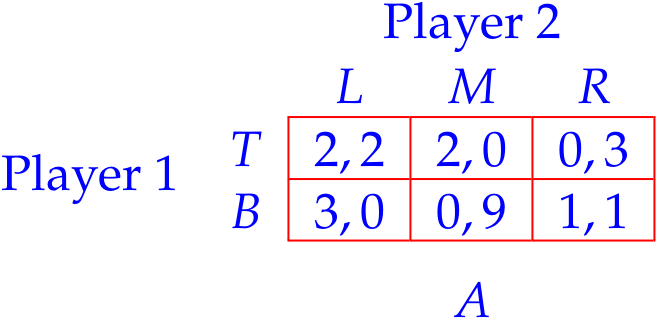
\includegraphics[scale=0.89]{sgamex1}\vspace{0.65mm}
\end{center}
}
\end{minipage}
\vspace{1mm}

\matrixsetoptions{w=1.2, h=0.6, force math}
\noindent\begin{minipage}{0.63\textwidth}
\begin{minted}{latex}
% xgames
\matrixsetoptions{w=1.2, h=0.6, force math}
\begin{matrixgame}[players, top={L, M, R}, left={T, B}, bottom=$A$]
	\payoffmatrix{2, 2 & 2, 0 & 0, 3\\ 3, 0 & 0, 9 & 1, 1}
\end{matrixgame}
\end{minted}
\end{minipage}\hspace{0.01\textwidth}%
\begin{minipage}{0.35\textwidth}
\fox*{
\begin{center}\vspace{-1.3mm}
\hspace{-4mm}\begin{matrixgame}[players, top={L, M, R}, left={T, B}, bottom=$A$]
	\payoffmatrix{2, 2 & 2, 0 & 0, 3\\ 3, 0 & 0, 9 & 1, 1}
\end{matrixgame}\vspace{-1.3mm}
\end{center}
}
\end{minipage}
\largeskip


The above is a comparison of the code and output between the strategic-form game in Figure~4 of the documentation of version 1.0 of the \texttt{sgamex} package. For a strategic-form game represented in a single payoff matrix, the code is relatively similar. Whether one prefers the compact input format of a list of optional arguments or a more modular approach using the key-value syntax and/or separate label commands will be a matter of taste. Note, however, that the code doubles with \texttt{sgamex} if there are two payoff matrices, whereas only one additional line is needed with this package.\largeskip

\newpage

\noindent
\begin{minipage}{0.7\textwidth}
\begin{minted}{latex}
% sgamex
\begin{game}{2}{2}
	&\rnode[t]{a12}{\(L\)} &\(R\)\\
	\Rnode[href=20]{a21}{\(T\)} &\(1,1\) &\Rnode{a23}{\(2,2\)}\\
	\(B\) &\rnode[b]{a32}{\(2,2\)} &\(3,3\)
\end{game}
\strike{a21}{a23}
\redStrike{a12}{a32}
\end{minted}
\end{minipage}\hspace{0.01\textwidth}%
\begin{minipage}{0.28\textwidth}
\fox*{
\begin{center}\vspace{7.5mm}
\hspace{-1mm}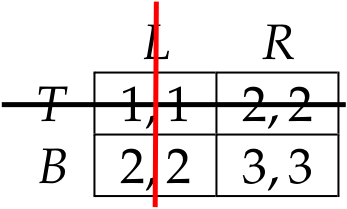
\includegraphics{sgamex2}\vspace{8.8mm}
\end{center}
}
\end{minipage}
\vspace{1mm}

\noindent
\begin{minipage}{0.7\textwidth}
\begin{minted}{latex}
% xgames
\begin{matrixgame}[top={L, R}, left={T, B}]
	\payoffmatrix{1, 1 & 2, 2\\ 2, 2 & 3, 3}
	\strike<2->{h}{1}
	\strike<3->{v}{1}
\end{matrixgame}
\end{minted}
\end{minipage}\hspace{0.01\textwidth}%
\begin{minipage}{0.28\textwidth}
\fox*{
\begin{center}\vspace{3.3mm}
\hspace{-3.5mm}\begin{matrixgame}[top={L, R}, left={T, B}]
	\payoffmatrix{1, 1 & 2, 2\\ 2, 2 & 3, 3}
	\strike<2->{h}{1}
	\strike<3->{v}{1}
\end{matrixgame}\vspace{4.8mm}
\end{center}
}
\end{minipage}
\largeskip

The above is a comparison of the code and output between the strategic-form game in Figure~10 of the documentation of version 1.0 of the \texttt{sgamex} package. When striking through actions, there are some advantages to this package. One need not define the nodes for the strikes manually, the strike command is overlay aware, and if the game is defined by several payoff matrices, the same actions is stricken through in all payoff matrices with a single \cmd{strike} command.

\subsection{Comparison to \texttt{egameps}}

\fox*{
\begin{center}
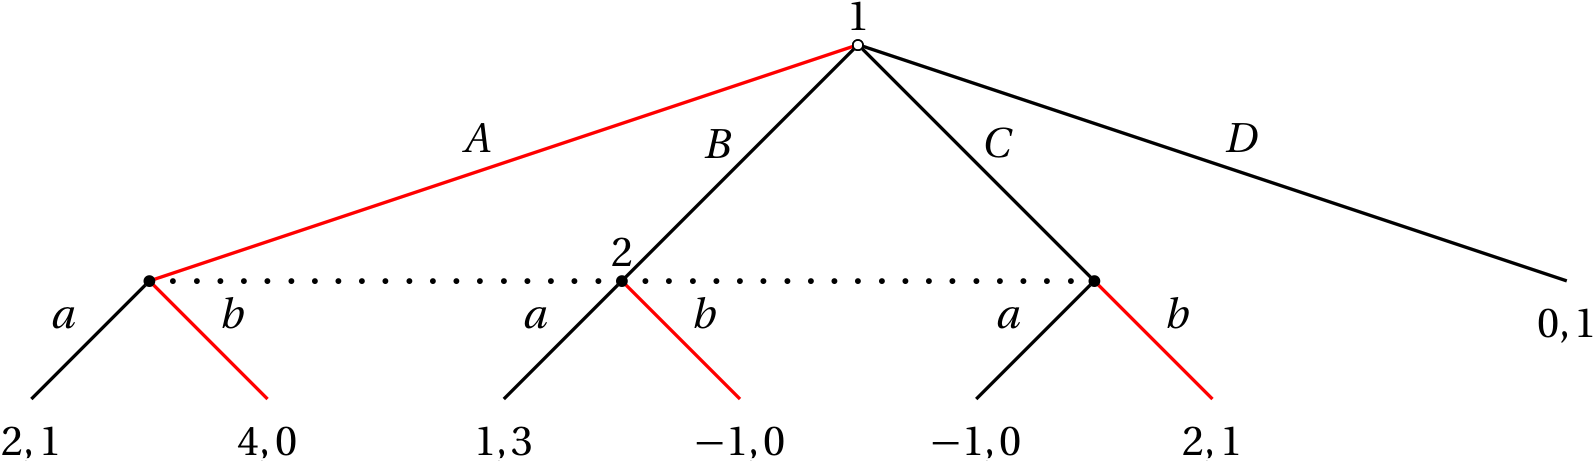
\includegraphics[scale=0.8]{egameps}
\end{center}
}

\begin{minted}{latex}
% egameps
\begin{egame}(1200,380)
	\putbranch(700,340)(3,1){600}
	\iib[linecolor=red][]{\(1\)}{\(A\)}{\(D\)}[][\(0,1\)]
	\initialtrue
	\putbranch(700,340)(1,1){200}
	\egactionlabelsep=0.5mm
	\iib{}{\(B\)}{\(C\)}
	\egactionlabelsep=1mm
	\putbranch(100,140)(1,1){100}
	\iib[][linecolor=red]{}{\(a\)}{\(b\)}[\(2,1\)][\(4,0\)]
	\putbranch(500,140)(1,1){100}
	\iib[][linecolor=red]{}{\(a\)}{\(b\)}[\(1,3\)][\(-1,0\)]
	\putbranch(900,140)(1,1){100}
	\iib[][linecolor=red]{}{\(a\)}{\(b\)}[\(-1,0\)][\(2,1\)]
	\infoset(100,140){800}{2}
\end{egame}
\end{minted}

\fox*{
\begin{center}
\begin{gametree}[nodes=full, root=hollow, labels=short, force math]
	\branch[player=1, root=w] from (0,0) to[v=1.6,h=3.2] {A<1->; B; C; D(0,1)};
	\branch[player=2, label=none] from (w1) to[v=0.9,h=1.5] {a(2,1); b<1->(4,0)};
	\branch from (w2) to {a(1,3); b<1->(-1,0)};
	\branch from (w3) to {a(-1,0); b<1->(2,1)};
	\informset[dashed] (w1) -- (w2) -- (w3);
\end{gametree}
\end{center}
}

\begin{minted}{latex}
% xgames
\begin{gametree}[nodes=full, root=hollow, labels=short, force math]
	\branch[player=1, root=w] from (0,0) to[v=1.8,h=3] {A<1->; B; C; D(0,1)};
	\branch[player=2, label=none] from (w1) to[v=1,h=1.5] {a(2,1); b<1->(4,0)};
	\branch from (w2) to {a(1,3); b<1->(-1,0)};
	\branch from (w3) to {a(-1,0); b<1->(2,1)};
	\informset[dashed] (w1) -- (w2) -- (w3);
\end{gametree}
\end{minted}
\vspace{-1mm}

The above is a comparison of the code and output of the extensive-form game in Figure~4 of the documentation of version 1.12 of the \texttt{egameps} package. There are numerous advantages to using this package over \texttt{egameps}. First and foremost, the coordinates of the individual branches do not have to be computed manually. This makes trees faster to draw and easier to adjust at a later point. Second, writing a tree is more straight-forward since one only ever needs the two rather self-explanatory commands \cmd{branch} and \cmd{informset}. Third, a \cmd{branch} can have any number of children. Fourth, highlighting strategies as well as drawing branches and information sets are all overlay aware. Finally, this package comes with additional features such as adding subgames, displaying the distribution over nodes induced by strategy profiles, and support for \TikZ's externalization library.

%\newpage

\subsection{Comparison to \texttt{istgame}}

\fox*{
\begin{center}\vspace{1mm}

\includegraphics[scale=0.95]{istgame}\vspace{1mm}
\end{center}
}

\begin{minted}{latex}
% istgame
\begin{istgame}
	\setistgrowdirection'{right}
	\xtdistance{20mm}{20mm}
	\istroot(0)[chance node]<180>{Chance}
	\istB<grow=north>{H}[l]{\pi}[r] \istB<grow=south>{L}[l]{1-\pi}[r] \endist
	\istroot(H0)(0-1)<180>{F}
	\istb{(p_1,E)}[a] \endist
	\istroot(L0)(0-2)<180>{F}
	\istb{(p_1,E)}[a] \endist
	\setistmathTF*001
	\cntmdistance*{10mm}{20mm}{8mm}
	\istroot(H)(H0-1)
	\istb{Buy}[br] \istb{Refrain}[ar]{-E,0} \endist
	\istrootcntm(H1)(H-1)
	\istb{$p_2^H$}[b] \istbm \endist
	\istroot(CH)(H1-1)<[label distance=-4pt]135>{C}
	\istb{Buy}[br]{p_1-E-c_H+p_2^H-c_H, 2H-p_1-p_2^H}
	\istb{Refrain}[ar]{p_1-E-c_H, H-p_1}
	\endist
	\istroot(L)(L0-1)
	\istb{Buy}[br] \istb{Refrain}[ar]{-E,0} \endist
	\istrootcntm(L1)(L-1)
	\istbm \istb{$p_2^L$}[a] \endist
	\istroot(CL)(L1-2)<[label distance=-4pt]-135>{C}
	\istb{Buy}[br]{p_1-E-c_L+p_2^L-c_L, 2L-p_1-p_2^L}
	\istb{Refrain}[ar]{p_1-E-c_L, L-p_1}
	\endist
	\xtInfoset(H)(L){C}[left]
\end{istgame}
\end{minted}

\treesetoptions{force math=false}

\fox*{
\begin{center}
\setplayernames[0]{Chance, F, C}
\begin{gametree}[horizontal, edge labels=inside]
	\branch[root=w] from (0,0) to[h=0, v=4, labels=outside] {$H$; $L$};
	\foreach[count=\i] \x in {H, L} {
		\branch[player=1] from (w\i) to[h=1.8, v=0, labels=outside] {$p_1, E$};
		\branch[player=2, label=none] from (w\i1) to[h=1.3, v=2] {Buy; Refrain(-E, 0)};
		\branch[player=1, label=135] from (w\i11) to[arc=40:-40:1.9] {30-20*\i:$p_2^\x$};
		\branch[player=2, label=405-270*\i] from (w\i111) to[h=1.3, v=2] {Buy(p_1-E-2c_{\x}+p_2^{\x}, 2\x-p_1-p_2^{\x}); Refrain(p_1-E-c_{\x}, \x-p_1)};
	}
	\informset[player=2, dashed, label=0.5] (w11) -- (w21);
\end{gametree}
\end{center}
}

\begin{minted}{latex}
% xgames
\setplayernames[0]{Chance, F, C}
\begin{gametree}[horizontal, edge labels=inside]
	\branch[root=w] from (0,0) to[h=0, v=4.2, labels=outside] {$H$; $L$};
	\foreach[count=\i] \x in {H, L} {
		\branch[player=1] from (w\i) to[h=1.8, v=0, labels=outside] {$p_1, E$};
		\branch[player=2, label=none] from (w\i1) to[h=1.3, v=2.2] {Buy; Refrain(-E, 0)};
		\branch[player=1, label=135] from (w\i11) to[arc=40:-40:1.9] {30-20*\i:$p_2^\x$};
		\branch[player=2, label=405-270*\i] from (w\i111) to[h=1.3, v=2] {Buy(p_1-E-2c_{\x}+p_2^{\x}, 2\x-p_1-p_2^{\x}); Refrain(p_1-E-c_{\x}, \x-p_1)};
	}
	\informset[player=2, dashed, label=0.5] (w11) -- (w21);
\end{gametree}
\end{minted}

The above is a comparison of the code and output of the extensive-form game in Section~16.10 of the  documentation of version 2.0 of the \texttt{istgame} package. The code is somewhat shorter with this package, even after discounting the for loop in the second piece of code. An advantage of this package is again that one only needs the two intuitive commands \cmd{branch} and \cmd{informset} to draw the tree. Moreover, all commands are overlay aware and coloring as well as labeling is automatic  and that those commands are overlay aware. Moreover, the key-value syntax may be easier to use than commands with a long sequence of parameters. A distinct advantage of the \texttt{istgame} package is that it compiles quicker. Drawing the above tree takes 0.151 seconds with \texttt{istgame} and 0.246 seconds with this package.\footnote{The test was performed over an average of 100 runs on a i9-10900K processor with the code by Phelype Oleinik at \url{https://tex.stackexchange.com/a/505840/203616}.}

%\newpage 

\section{Frequently Asked Questions}
\vskip-3mm

\question I get a whole bunch of \texttt{\textbackslash GenericError}s or other confusing errors.

\answer There are three likely causes for this:
\begin{itemize}
\item The actions specified in a \texttt{gametree} involve characters that are not allowed in the name of a \TikZ node while the \texttt{index=action} is active. The easiest solution is to set \texttt{index=number} instead. 
\item You are using a non-expandable macro like \cmd{mathcal} or \cmd{sqrt} in an \texttt{autolabel} or in any label within an \cmd{xforeach} loop. The solution is to precede all non-expandable macros by a \cmd{noexpand}. %Testing whether a label is expandable is equivalent to the halting problem, so I can't think of a way to catch this error. 
\item There may be other expansion issues in the code that I have not caught yet. If the bug arises when you use non-expandable macros in any other kind of label, most likely you can again fix the issue by preceding all non-expandable macros by a \cmd{noexpand}.
\item There is some other bug in the package's code. Even though I may not always respond immediately, I~appreciate emails with bug reports because I want this package to be bug free eventually. 
\end{itemize}



\end{document}




